\documentclass[11pt]{article}
\usepackage{amsgen,amsmath,amstext,amsbsy,amsopn,amssymb}
\usepackage[dvips]{graphicx}
\usepackage{extarrows}
\usepackage[thmmarks]{ntheorem}
\usepackage{mdframed}
\usepackage{amsmath}
%% \usepackage[round]{natbib}
%\usepackage[pdftex]{hyperref}
\usepackage{hyperref}
\hypersetup{
    colorlinks=true,       % false: boxed links; true: colored links
    linkcolor=blue,        % color of internal links
    citecolor=blue,        % color of links to bibliography
    filecolor=blue,        % color of file links
    urlcolor=blue          % color of external links
}


%------------------

\newcommand {\Reals}  {{\rm I \! R}}
\newcommand {\Naturals}  {{\rm I \! N}}
\newcommand {\reals}  {{\rm I \! R}}
\newcommand {\Rationals}  {{\rm I \! Q}}
\newcommand {\Integers}  {{\rm I \! Z}}


\theoremstyle{numberplain}
\newmdtheoremenv{lem}{Lemma}
\newmdtheoremenv{code}{Code}
\newmdtheoremenv{claim}{Claim}


%\newframedtheorem{ques}{Question}


\theoremstyle{nonumberplain}
\newmdtheoremenv{ques}{Question}
\theoremsymbol{$\diamondsuit$}

\newtheorem{proof}{Proof}

\newmdtheoremenv{State}{}	


\theorempostskipamount=5pt
\def\theoremframecommand{ %
\psshadowbox[linecolor=black]}
\newtheorem{rem}{Remark}
\newtheorem{ans}{Answer}
\pagestyle{headings}


\title{CIS 502}
\author{Yezheng Li}
%----------------
\def\half{{\frac12}}
\def\Star{{$(\ast)$~~}}
\def\as{{\ast}}

\newcommand{\dps}{\displaystyle}
\newcommand{\cel}[1]{{\lceil {#1} \rceil}}
\newcommand{\flr}[1]{{\lfloor {#1} \rfloor}}
\newcommand{\opt}[1]{{\tt opt}(}
\def\ve{{\varepsilon}}




\newcommand{\bbR}{\mathbb{R}}
\newcommand{\cC}{\mathcal{C}}
\newcommand{\cS}{\mathcal{S}}
\newcommand{\cT}{\mathcal{T}}
\newcommand{\cU}{\mathcal{U}}
\newcommand{\cV}{\mathcal{V}}
\newcommand{\Ra}{{\mathcal{R}}}
\newcommand{\Null}{{\mathcal{N}}}
\newcommand{\Range}{{\mathcal{R}}}

\newcommand{\0}{{\mathbf{0}}}
\renewcommand{\a}{{\mathbf{a}}}
\renewcommand{\b}{{\mathbf{b}}}
\newcommand{\e}{{\mathbf{e}}}
\newcommand{\f}{{\mathbf{f}}}
\renewcommand{\u}{{\mathbf{u}}}
\renewcommand{\v}{{\mathbf{v}}}
\newcommand{\w}{{\mathbf{w}}}
\newcommand{\x}{{\mathbf{x}}}
\newcommand{\y}{{\mathbf{y}}}
\newcommand{\yhat}{{\mathbf{\hat{y}}}}
\newcommand{\z}{{\mathbf{z}}}
\newcommand{\A}{{\mathbf{A}}}
\newcommand{\B}{{\mathbf{B}}}
%\newcommand{\C}{{\mathbf{C}}}
\newcommand{\D}{{\mathbf{D}}}
\renewcommand{\H}{{\mathbf{H}}}
\newcommand{\I}{{\mathbf{I}}}
\newcommand{\M}{{\mathbf{M}}}
\newcommand{\E}{{\mathbf{E}}}
\renewcommand{\P}{{\mathbf{P}}}
\newcommand{\Q}{{\mathbf{Q}}}
\newcommand{\R}{{\mathbf{R}}}
\renewcommand{\S}{{\mathbf{S}}}
\newcommand{\T}{{\mathbf{T}}}
%\newcommand{\U}{{\mathbf{U}}}
\newcommand{\V}{{\rm V}}
\newcommand{\Var}{{\rm Var}}
\newcommand{\W}{{\mathbf{W}}}
\newcommand{\X}{{\mathbf{X}}}
\newcommand{\Y}{{\mathbf{Y}}}
\newcommand{\Z}{{\mathbf{Z}}}
\newcommand{\betahat} {{b}}   % could be {{\hat{\beta}}}

\newcommand{\tX}{{\mathbf{\tilde{X}}}}
\newcommand{\tu}{{\mathbf{\tilde{u}}}}
\newcommand{\tv}{{\mathbf{\tilde{v}}}}

\newcommand{\bX}{{\mathbf{\bar{X}}}}
\newcommand{\by}{{\mathbf{\bar{y}}}}

\newcommand{\cR}{{\cal R}}
\newcommand{\cN}{{\cal N}}
\begin{document}
\maketitle
\tableofcontents
\section{Ch2}

\begin{ques}(Fall 2014-I, 20 Points) You are given a binary tree which satisfies the (min) heap property: the
parent is smaller than both the children. It is not a search tree and need not be balanced. The
number of elements in the heap is $n$. At each node, you can only see the value at the node and
follow the left or right pointers to the respective children.\par 
You want to know if the $k^{th}$ smallest element in the heap is less than the value $y$. Give a
worst case $O(k)$ time algorithm. The algorithm cannot depend on $n$. Your algorithm only needs to output yes/no.\par 
 You do not need to output that element. \par 
You need to give reasons why your answer is correct.
\end{ques}
\begin{ans} To count the number of nodes with value less than y.
Apply BFS with extra rules:
\begin{enumerate}
\item if confronting a node with element larger than $y$, stop searching that branch since its descendants have elements larger than $y$);
\item if {\tt counter}$\geq k$ return FALSE (and stop searching);
\item return TRUE.
\end{enumerate}
\end{ans}
\section{Ch4 Greedy algorithm}
\begin{ans}[HW1, 4-6, refers to \cite{solcornell}]
Let the contestants be numbered $1, \ldots, n$,
and let $s_i, b_i, r_i$ denote the swimming, biking, and
running times of contestant $i$.
Here is an algorithm to produce a schedule:
\begin{quote}
Arrange the contestants in order of decreasing $b_i + r_i$,
and send them out in this order.
\end{quote}
We claim that this order minimizes the completion time.

\begin{proof}
Suppose not, that is there exists an optimal schedule $S$ not using this order.
Then optimal schedule $S$ must contain two contestants $i$ and $j$ so that $j$ is sent out
directly after $i$, but $b_i + r_i < b_j + r_j$. We will call such a pair $(i,j)$ an {\em inversion}.
Consider the schedule $S'$ obtained by swapping the orders of $i$ and $j$.\par 
In this schedule $S'$ from swaping $i\& j$ in $S$, $j$ completes earlier than he/she used to.
Also, in the swapped schedule, $i$ gets out of the pool in $S'$ when $j$ got out of the pool in $S$;
but since $b_i + r_i < b_j + r_j$, $i$ finishes
sooner in $S'$ than $j$ finished
in $S$.
Hence $S'$ does not have a greater
completion time, and so it too is optimal.
\par 
Continuing in this way, we can eliminate all
inversions without increasing the completion time.
At the end of this process, we will have a 
schedule in the order produced by our algorithm,
whose completion time is no greater than that of
the original optimal order we considered.
Thus the order produced by our algorithm must
also be optimal.
\end{proof}
\end{ans}

\begin{ans}[4-11, refers to \cite{solcornell}]
Label the edges arbitrarily as $e_1, \ldots, e_m$
with the property that $e_{m-n+1}, \ldots, e_m$
belong to $T$.
Let $\delta$ be the minimum difference between
any two non-equal edge weights;
subtract $\delta i / n^3$ from the weight of edge $i$.
Note that all edge weights are now distinct,
and the sorted order of the new weights is the
same as some valid ordering of the original weights.
Over all spanning trees of $G$, $T$ is the one whose
total weight has been reduced by the most;
thus, it is now the unique minimum spanning tree
of $G$ and will be returned by Kruskal's algorithm
on this valid ordering.
\end{ans}

\begin{ans}[HW1, 4-12](a) False by referring $(0,1), (6000,2)$ with $r=3000$.\par 
(b) Order the streams by ascent $\frac{b_i}{t_i},i=1,\ldots,n$.
\begin{proof} Suppose not. Consider the schedule of OPT not following the greedy order since it is feasible and greedy is not. Then there exists two adjacent jobs $i, j$ in OPT which were scheduled in the
order not preferred by greedy. Suppose OPT started transmitting $i$ first at time $t_0$
and had already sent $b_0$ bits by then. Since OPT is feasible then

$$
b_0\leq rt_0, b_0 + b_i \leq  r(t_0 + t_i), b_0+ b_i + b_j \leq r(t0 + t_i + t_j),
$$
and $b_it_j > b_j t_i$.\par 
\begin{State}
Swap order of $i$ and $j$ also provides a feasible solution.
\end{State}
\begin{proof}Suppose not, that is, $b_0 + b_j > r(t_0 + t_j)$. Then 
$$b_i=(b_0 + b_i + b_j))- (b0 + bj) < r(t_0 + t_i + t_j)- r(t_0 + t_j )=rt_i,$$
then $\frac{b_j}{t_j}<\frac{b_i}{t_i}<r$ implies $b_0 + b_j < r(t_0 + t_j)$. A contradiction.\par 
\end{proof}
\end{proof}
\end{ans}

\begin{ans}[HW1, 4-13]
Below is to derive the sort order from the equations ( of course this would work easily only
in cases where the sort order is fixed - but that is the case here).\par 
Consider some sort order and we have a pair of adjacent jobs $i, j$ in the solution of OPT which violate
the order. If job $i$ went first and started at time $t$ then the contribution of the two jobs to the total weighted completion time is
$$w_i(t + t_i) + w_j(t + t_i + t_j);$$
If we performed a swap to $j, i$ (keeping everything else the same) then the contributions of all other jobs
would remain the same, and the contribution of these two would be
$$w_j(t + t_j) + w_i(t + t_i + t_j);$$
The second term would be smaller or equal (this is the condition needed to prove that the swap does not
make things worse) when
$w_j(t + t_j) + w_i(t + t_i + t_j) < w_i(t + t_i) + w_j(t + t_i + t_j),$
which turns out to be just $w_it_j < w_j t_i$. Which means schedule in the nonincreasing order of $wj=tj$.
\end{ans}

\begin{ans}[HW1, 4-15]

\begin{enumerate}
\item Sort everyone by the (nondecreasing) finish time. This is sequence $F$;
\item Also Sort everyone by the (nondecreasing) start time. This is sequence $S$;
\item Find the First finish time in F, say it is fi corresponding to job i. A committee member must have
started his/her shift by then.
\item Consider all the jobs in $S$ which start by $f_i$. Among these choose the person who finishes last say $\sigma(i)$.
Choose this person in the committee. Note that if the optimum chose differently then this person can
oversee the same set of persons overseen by the committee member chosen by the optimum. Remember
the last seen element of $S$ so far, say $s$.
\item  Continue along $F$ and mark every person who finishes before $\sigma(i)$ as overseen.
\item  repeat
\begin{enumerate}
\item Consider the next person in $F$ (who is not yet overseen) say this is $f_j$ .
\item Starting after $s$ in Step 4, find all persons who starts before $f_j$ in S. This person may have already
been overseen. Remember the person who finishes last (say $\sigma(j)$) and the new value of $s$.
\item Continue along $F$ and mark every person who finishes before $\sigma(j)$ as overseen.
\end{enumerate}
\item until $F =\emptyset $.
\end{enumerate}
Running time $O(n\log n)$ as well.
\end{ans}



\begin{ques}[HW2,4-17]
Consider the following variation on the Interval Scheduling Problem. You have a processor that can operate 24 hours a day, every day. People submit request to run daily jobs on the processor. Each such job comes with a start time and an end time; if the job is accepted to run on the processor, it must run continuously, every day, for the period between its start and end times. (Note that certain jobs can begin before midnight and end after midnight; this makes for a type of situation  different from what we saw in the Interval Scheduling Problem.)\par
Given a list of $n$ such jobs, your goal is to accept as many jobs as possible (regardless of their length), subject to the constraint that the processor can run at most one job at any given point in time. Provide an algorithm to do this with a running time that is polynomial in $n$. You may assume for simplicity that no two jobs have the same start or end times. 
\end{ques}
\begin{ans}[refers to \cite{solcornell}]
Here is the algorithm where $T_{\text{all}}$ represent the $24$--hour time.
\begin{enumerate}
\item Input $I_1, \ldots, I_N$, $N$ intervals/ requests of time, represented by $I_j\doteq (t_{\text{start}}, t_{\text{end}})$;
\item For $j=1,\ldots, N$
\begin{enumerate}
\item Denote by $S_j$, the set of intervals/ requests selected; by $A_j$, the set of intervals/ requests still available;\par 
(initialization) $S_j\leftarrow \{I_j\}$, $A_j\leftarrow \{I_k:k=1,\ldots, N, I_k\cap I_j=\emptyset \}$;
\item Notice $T_{\text{all}}\setminus I_j$ can be regarded as a line when rest of the intervals are to be scheduled selectively. According to classic interval/request scheduling problem, $S, A$ can be modified by first-finish-first schedule routine.
\end{enumerate}
\item Compare $\# S_j$ and select $\dps j_0\in arg\max_{j=1,\ldots,N} \# S_j$, namely the index $j_0$ for which we can schedule with as many intevals/ requests as possible;
\item Output $S_{j_0}$.
\end{enumerate}
\textbf{Running time:}
\end{ans}
\begin{ques}[HW2,4-20]Every September, somewhere in a far-away mountainous part of the world, the county highway crews get together and decide which roads to keep clear through the coming winter. There are $n$ towns in this county and the road system can be viewed as a (connected) graph $G=(V,E)$ on this set of towns, each representing a road joining two of them. In the winter, people are high enough up in the mountains that they stop worrying about the \textcolor{blue}{length} of roads and start worrying about their \textcolor{blue}{altitude} -- this is really what determines how difficult the trip will be. \par
So each road -- each edge $e$ in the graph -- is annotated with a number $a_e$ that gives the altitude of the hightest point on the road. We will assume that no two edges have exactly the same altitude value $a_e$. The height of a path $P$ in the graph is then the maximum of $a_e$ over all edges $e$ on $P$. Finally, a path between towns $i$ and $j$ is declared to be \textcolor{blue}{winter-optimal} if it achieves the minimum possible height over all paths from $i$ to $j$.\par
The highway cres are going to select a set $E'\subset E$ of the roads to keep clear through the winter; the rest will be left unmaintained and kept off limits to travellers. They all agree that whichever subset of roads $E'$ they decide to keep clear, it should have the property that $(V,E')$ should be no greater than it is in the full graph $G=(V,E)$. We will say that (V,E') is a \textcolor{blue}{minimum-altitude connected subgraph}  if it has this property.\par
Given that they are going to maintain this key property, however, they otherwise want to keep as few roads clear as possible. One year, they hit upon the following conjecture:
\begin{itemize}
\item 
The minimum spaning tree of $G$, with respect to the edge weights $a_e$, is a minimum-altitude connected subgraph.
\end{itemize}
(In an earlier problem, we claimed that there is a unique minimum spanning tree when the edge weights are distinct. Thus, thanks to the assumption that all $a_e$ are distinct, it is okay for us to speak of the minimum spanning tree.)\par
Initially, this conjecture is somewhat counterintuitive, since the minimum spanning tree is trying to minimize the \textcolor{blue}{sum} of the values $a_e$, while the goal of minimizing altitude seems to be asking for a fairly different thing. But lacking an argument to the contrary, they begin considering an even bolder second conjecture:
\begin{itemize}
\item \textcolor{blue}{ 
A subgraph $(V,E')$ is a minimum--altitude connected subgraph if and only if it contains the edges of the minimum spanning tree.
}
\end{itemize}
Note that this second conjecture would immediately imply the first one, since a minimum spanning tree contains its own edges.\par
So here is the question.
\begin{enumerate}
\item Is the first conjecture true, for all choices of $G$ and distinct altitudes $a_e$? Give a proof or a counterexample with explanation.
\item Is the second conjecture true, for all choices of $G$ and distinct altitudes $a_e$? Give a proof or a counterexample with explanation. 
\end{enumerate}
\end{ques}
\begin{ans}
\begin{enumerate}
\item True. By exercise 4-8, the minimal spanning tree is unique and can be obtained by Kruskal's algorithm. The thing to show is that Kruskal's algorithm also produces a \textcolor{blue}{minimum-altitude connected subgraph}. It suffices to show counterpart of lemma 4.17:
\begin{lem}[4.17'] Let $S$ be any subset of nodes that is neighter empty nor equal to all of $V$ and let edge $e=(v,w)$ be the minimum--cost edge with one end in $S$ and the other in $V-S$. There exists a minimum spanning tree containing the edge $e$.
\end{lem}
\begin{proof} Suppose not, that is any spanning tree $T$ containing $e$ cannot be a minimal--altitude subgraph.\par 
Given ang minimal--altitude subgraph $T_1$. In order to show there exists a tree $T_2$ containing $e$ that has at most the same altitude, an exchange argument is applied:\par 
The crux is therefore to find an edge that can be successfully exchanged with $e$. Recall that the ends of $e$ are $v\in S,w\in V-S$. That $T_1$ is connected infers there exists a path $P$ in $T$ from $v$ to $w$. Starting at $v$, suppose first node in $V-S$ of $P$ in sequence $v\rightarrow w$ is $w'$ and $v'\in S$ be previous node of $w'$. Denote $e'=(v',w')$, an edge of $T_1$ with one end in $S$ and the other in $V-S$. \par 
Exchange of $e$ and $e'$ produces $T_2=(T_1-\{e'\})\cup \{e\}$. $T_2$ is also a spanning subgraph since:
\begin{enumerate}
\item Clearly it is connected since $(V,T_1)$ is connected and that any path in $(V,T_2)$ that used the edge $e'$ can now be "rerouted" in $(V,T_2)$;
\item It is also acyclic since the only cycle in $(V, T_2\cup\{e'\}$ is the one composed of $e$ and the path $P$ and this cycle is not present in $(V,T_2)$ due to the deletion of $e'$.
\end{enumerate}
Note that $a_e\leq a_{e'}$ implies altitude of $(V,T_2)$ is less equal to that of $(V,T_1)$; specifically, $(V,T_2)$ is also a \textcolor{blue}{minimal--altitude connected subgraph} and contains $e$. This leads to a contradiction!\par
Therefore, there exists a minimum spanning tree containing edge $e$.
\end{proof}	
\item True. We show that 
\begin{quote}
every edge added by Kruskal's algorithm has to
be added to the min-altitude subgraph.
\end{quote}
\begin{proof}
Suppose not. Let $(u,v)$ be the first time we add an edge in Kruskal's algorithm which is not in our
min-altitude subgraph. Consider the cut defined by the edge $(u,v)$ say $S, V\setminus S$  (where $S$ corresponds to the nodes in the subtree connected to $u$). By (4-17), every other edge that spans the cut has altitude more than that of $(u, v)$. So the minimum altitude path between $u$ and $v$ itself must be the edge $(u, v)$. Thus we have a contradiction to the min-altitude subgraph property for this pair.
\end{proof}
We now show that 
\begin{quote}
the min-altitude subgraph is a tree, provided that the weights are distinct. 
\end{quote}
\begin{proof}
Suppose not. Consider a cycle -- the highest altitude edge can be deleted without affecting the connectivity in any
way. Therefore the min-altitude subgraph is exactly the minimum spanning tree.
\end{proof}
\end{enumerate}
\end{ans}
\newpage
\begin{ques}[HW2, 4-21] Let us say that a graph $G=(V,E)$ is a \textcolor{blue}{near-tree} if it is connected and has at most $n+8$ edges, where $n=|V|$. Give an algorithm with running time $O(n)$ that takes a near-tree $G$ with costs on its edges, and returns a minimum spanning tree of $G$. You may assume that all the edge costs are distinct.
\end{ques}
\begin{ans}
Use the cycle property: that given any cycle there exists a minimum spanning tree that
does not use the heaviest edge in that cycle.\par 
\begin{enumerate}
\item ensure that the graph is connected in $O(n+n+8) = O(n)$ time;
\item use favourite algorithm
to find a cycle (BFS/DFS) and can find a cycle in $O(n + m) = O(n + n + 8) = O(n)$ time;
\item delete one edge. We now have $n + 7$ edges. 
\end{enumerate}
Repeat this step for 8 more steps, we will have $n -1$ edges left.At this point we must have a tree since the graph is connected. The total running time is $9 \cdot O(n) = O(n)$.
\end{ans}
\begin{ans}[\textcolor{red}{HW2,4-28}]
%
%Let GX be the graph on the X edges and GY be the graph on Y edges. Suppose both GX and
%GY are individually connected. Then we can choose a connected subtree from GX with k + 1 nodes (we
%can start from an spanning tree of X and start deleting leaves). If we compress these nodes nodes into one
%supervertex X0.
%Dene a graph G0
%Y such that: If (u; v) was an edge in GY and u 2 X0; v 62 X0 then we add the edge
%(X0; v) in G0
%Y . If (u; v) was an edge in GY and u; v 62 X0 then we add the edge to G0
%Y . Observe that G0
%Y is
%connected (since GY was connected). We now pick a spanning tree in G0
%Y which has only n 􀀀 k 􀀀 1 edges
%from Y . This runs in time O(n + m).
%Therefore the question reduces to: What do we do when either GX or GY are not individually connected?
%Suppose GX is not connected. We rst shrink the connected components of GX into supervertices |
%if there is more than n 􀀀 k supervertices then we cannot choose n 􀀀 k 􀀀 1 edges from Y and connect
%the supervertices (and therefore connect the graph), we output \not possible". Suppose the number of
%supervertices is z  n 􀀀 k. We now consider the graph G0
%Y where these supervertices are shrunk (dened as
%above) and nd a spanning tree { if no such spanning tree exists then we output \not possible". Otherwise
%we have chosen z 􀀀 1 edges from Y , say this set is S1.
%Now focus on the graph G1(X);G1(Y ) where we collapse the vertices connected by S1 into connected
%components. Observe that G1(X) is now connected. We now have reduced our problem to n0 = n􀀀jS1j and
%G = G1.
%Therefore, we only need to assume that GY is not connected. We now consider the connected components
%of GY . Again, these cannot be more than k + 1 in number and if we shrink them, they must be connected
%by a spanning tree in G0
%X. In either case we output \not possible". We can again choose S2 edges from X
%such that jS2j  k and adding these edges will connect GY .
%Now we collapse both edge sets S1; S2 and have a problem where n0 = n􀀀jS1j􀀀jS2j and k0 = k􀀀jS2j. We
%can now use the rst solution which assumes GX;GY are both connected. Overall running time: O(n+m).
%2
\end{ans}

\begin{ques}[HW3,4-31, variant of Kruskal's algorithm] Since Minimum Spanning Tree Problem is somehow related with shortest $u-v$ path, following variant of Kruskal's algorithm is designed:
\begin{enumerate}
\item Sort all the edges in order of increasing length (assume all edge lengths are distinct except that $d_{uv}=\infty$ once they are disconnected in certain graph);
\item construct a subgraph $H=(V,F)$ by considering each edge in order (from short to long);
\item when it comes to edge $e=(u,v)$, add $e$ once $3 l_e<d_{uv}$.
\end{enumerate}
Speaking of subgraph $H=(V,F)$ it produced:
\begin{enumerate}
\item Prove that for every pair of nodes $u,v\in V$, the length of the shortest $u-v$ path in $H$ is at most three times the length of the shortest $u-v$ path in $G$;
\item Despite its ability to approximately preserve shortest--path distances, the subgraph $H$ cannot be too dense. Let $f(n)$ denote the maximum number of edges that can possibly be produced as the output of this algorithm, over all $n$-- node input graphs with edge lengths. Prove that$\dps \lim_{n\rightarrow \infty}\frac{f(n)}{n^2}=0$.
\end{enumerate}
\end{ques}
\begin{ans}
\begin{enumerate}
\item Denote a shortest path in $G=(V,E)$ between $v_1, v_2\in V$ by
$$P_{12}\doteq e_{i_0i_1}e_{i_1 i_2}\ldots e_{i_{m-1} i_m}\xlongequal{i_0=1,i_m=2}e_{1i_1}e_{i_1 i_2}\ldots e_{i_{m-1} 2},
$$
where $\{e_{i_ki_{k+1}}\doteq (v_{i_k}, v_{i_{k+1}}) \}_{k=0}^{m-1}\subset E,\{v_{i_k} \}_{k=0}^m\subset
 V$ and $\dps \sum_{k=0}^{m-1}l_{e_{i_k i_{k+1}}}$ is the length of $P_{12}$.\par
Speaking of any $e_{i_k i_{k+1}}\in E\setminus F$ (or alternatively,$\in G\setminus H$) , there exists \textcolor{red}{$P'_{i_k i_{k+1}}$} $\subset F$, \textcolor{red}{another path} (\textcolor{red}{red notation} in figure \ref{fig:path12} which as a matter of fact, could be shortest path between $v_{i_k}, v_{i_{k+1}}$ in $H$).  In all, whatever $e_{i_k i_{k+1}}\in F$ or not, there exists a path in $H$ such that its length is smaller than $3\dps \sum_{k=0}^{m-1}l_{e_{i_k i_{k+1}}}$.
\begin{figure}
\begin{center}
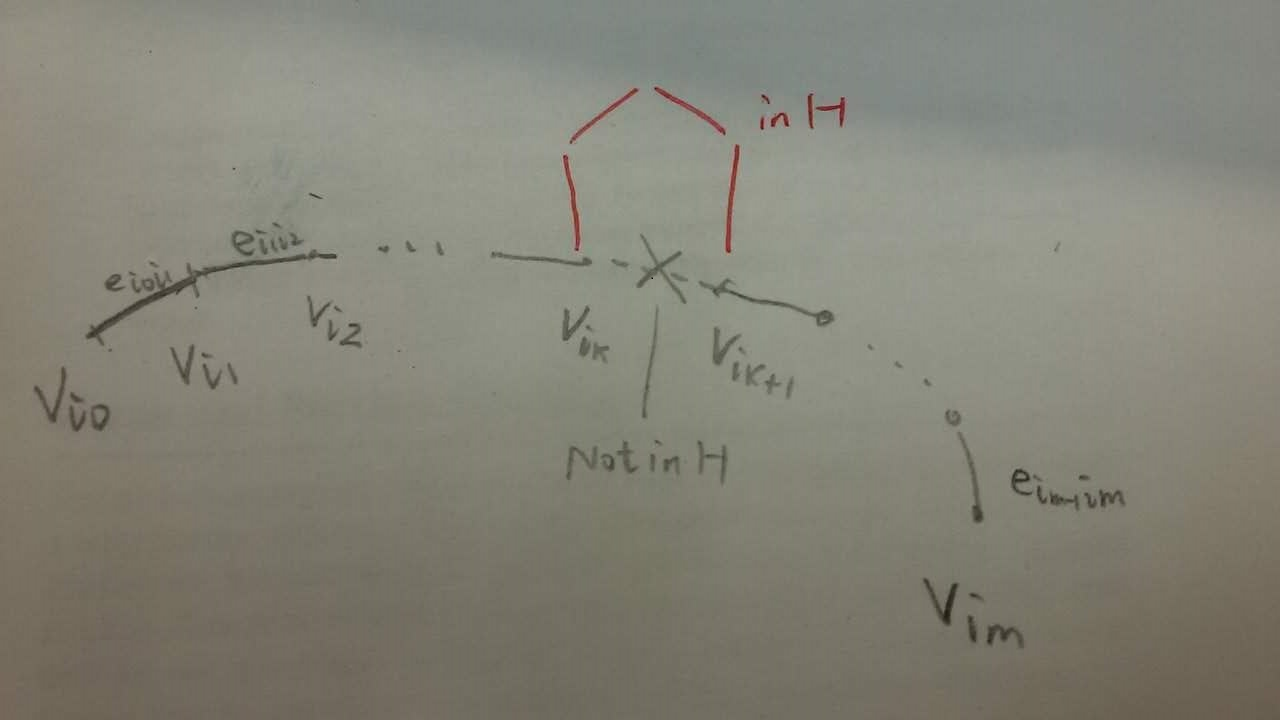
\includegraphics[width=\textwidth]{4_31_a.jpg}
\end{center}
\caption{$P_{12}$, one of shortest paths between $v_1$, $v_2$ in $G=(V,E)$.}
\label{fig:path12}
\end{figure}
\item \textbf{(refers to \cite{solcornell})} \begin{lem}
Cycle in $H$ has at least 5 	edges.
\label{lem: cycle in H has at least 5 edges}
\end{lem}
\begin{proof}
Suppose not and $C$ is such a cycle while $e = (u,v)$ is the last edge added to it. Then at the moment $e$ was considered, there was a $u$-$v$ path $Q_{uv}\in H=(V,F)$  of at most three edges, on which each edge had length at most $\ell_e$. Thus $\ell_e$ is not less than a third the length of $Q_{uv}$, and so it should not have been added.
\end{proof}
\begin{lem}
An $n$-node graph $H$ with no cycle of length $\leq 4$ must contain a node of degree at most $\sqrt{n}$.
\label{lem:min degree Q4-31}
\end{lem}
\begin{proof}
Suppose not and consider any node $v$ of $H$. Let $S(v)\doteq \{u\in V: (u,v)\in F\}$, set of neighborhood of $v$ and $\# S(v)=|S(v)|>\sqrt{n}$. Notice that there is no edge joining two nodes of $S(v)$, or we would have a cycle of length $3$. Now let $N(S(v))\doteq \{u\in V: S(u)\cap S(v)\neq\emptyset\}$, set of all nodes with a neighbor in $S(v)$. Since $H$ has no cycle of length $4$, each node in $N(S)$ has exactly one neighbor in $S(v)$. But $|S(v)| > \sqrt{n}$, and each node in $S$ has $\geq \sqrt{n}$ neighbors other than $v$, so we would have $|N(S(v))| > n$, a contradiction. 
\end{proof}
\begin{proof}[1, for $2^{nd}$ part of statement; refers to \cite{solcornell}] Now, if we let $g(n)$ denote the maximum number of edges in an $n$-node graph with no cycle of length $4$, then $g(n)$ satisfies the recurrence $g(n) \leq g(n-1) + \sqrt{n}$ by deleting the lowest-degree node and lemma \ref{lem:min degree Q4-31}, and so we have $g(n) \leq n^{3/2} = o(n^2)$.
\end{proof} 


\begin{proof}[2, for $2^{nd}$ part of statement; refers to \cite{solcornell}]
Suppose not. $H$ has at least $\ve n^2$ edges, then the sum of all degrees is $2 \ve n^2$, $\xLongrightarrow{\text{lemma \ref{lem: cycle in H has at least 4 edges}}}$ there is a set $S$ of at least $\ve n$ nodes each of whose degrees is at least $\ve n$.
Now, consider the set $Q$ of all pairs of edges $(e,e')$ such $e$ and $e'$ each have an end equal to the same node in $S$. We have $|Q| \geq \ve n {{\ve n} \choose 2}$, since there are at least $\ve n$ nodes in $S$, and each contributes at least ${{\ve n} \choose 2}$ such pairs. For each edge pair $(e,e') \in Q$, they have one end in common;
we {\em label} $(e,e')$ with the pair of nodes at their other ends.
%Now, label each pair in $Q$ with the pair of nodes at the other
%end of the two edges.
Since $|Q| > {n \choose 2}$ for sufficiently large $n$, the pigeonhole principle implies that some two pairs of edges $(e,e'), (f,f') \in Q$ receive the same label. But then $\{e, e', f, f'\}$ constitutes a four-node cycle. For a second proof, we observe that an $n$-node graph $H$ with no cycle of length $\leq 4$ must contain a node of degree at most $\sqrt{n}$. For suppose not, and consider any node $v$ of $H$. Let $S$ denote the set of neighbors of $v$. Notice that there is no edge joining two nodes of $S$, or we would have a cycle of length $3$. Now let $N(S)$ denote the set of all nodes with a neighbor in $S$. Since $H$ has no cycle of length $4$, each node in $N(S)$ has exactly one neighbor in $S$. But $|S| > \sqrt{n}$, and each node in $S$ has $\geq \sqrt{n}$ neighbors other than $v$, so we would have $|N(S)| > n$, a contradiction. Now, if we let $g(n)$ denote the maximum number of edges in an $n$-node graph with no cycle of length $4$, then $g(n)$ satisfies the recurrence $g(n) \leq g(n-1) + \sqrt{n}$ (by deleting the lowest-degree node), and so we have $g(n) \leq n^{3/2} = o(n^2)$.
\end{proof} 
\end{enumerate}
\end{ans}
\begin{rem}
\begin{enumerate}
\item Suppose not. Denote a shortest path in $H=(V,F)$ between $v_1, v_2\in V$ by
$$p_{12}=e_{i_0i_1}e_{i_1 i_2}\ldots e_{i_{m-1} i_m}\xlongequal{i_0=1,i_m=2}e_{1i_1}e_{i_1 i_2}\ldots e_{i_{m-1} 2},
$$
where $\{e_{i_ki_{k+1}}\doteq (v_{i_k}, v_{i_{k+1}}) \}_{k=0}^{m-1}\subset F\subset E,\{v_{i_k} \}_{k=0}^m\subset
 V$ but $\dps d_{v_1v_2}=\sum_{k=0}^{m-1}l_{e_{i_k i_{k+1}}}$, the length of $p_{12}$ is more than three times of the shortest-path length between $v_1,v_2$  in $G=(V,E)$.\par
Notice $p_{i_j i_k}\doteq e_{i_ji_{j+1}}e_{i_{j+1} i_{j+2}}\ldots e_{i_{k-1} i_k} (j<k)$ is also one of the  shortest paths between $v_{i_j},v_{i_k}$. Then above background infers: $\exists k_0\in [m]$ such that 
$l_{e_{i_{k_0} i_{k_0+1}}}$ is more than the shortest-path lengths between $v_{i_{k_0}}$, $v_{i_{k_0+1}}$ in $G$.
\end{enumerate}
\end{rem}
\begin{ques}[HW3,4-32, variant of minimum-cost arborescence algorithm] Consider a directed graph $G=(V,E)$ with a root $r\in V$ and nonnegative costs on the edges. In this problem we consider variants of the minimum-cost arborescence (MCA) algorithm.
\begin{enumerate}
\item MCA algorithm discussed in section 4.9 of \cite{jon2005algorithm} works as follows. We modify the costs, consider the subgraph of zero-cost edges, look for a directed cycle in this subgraph, and contract it (if one exists). Argue briefly that instead of looking for cycles, we can instead identify and contract strong components\footnote{From \cite{wikipedia}, a graph is said to be strongly connected if every vertex is reachable from every other vertex.} of this subgraph;
\item  After defining $y_v$ to be the minimum cost of an edge entering $v$ and we modified the costs of all edges $e$ entering node $v$ to be $c_e''\doteq \max (0,c_e-2y_v)$ instead of $c_e'\doteq c_e-y_v$. This new change is likely to turn more edges to $0$ cost. Suppose now we find an arborescence $T$ of $0$ cost. Prove that this $T$ has cost at most twice the cost of the MCA in the original graph;
\item Assume you do not find an arborescence of $0$ cost. Contract all $0-$ cost strong components and recursively apply the same procedure on the resulting graph until an arborescence is found. Prove that this $T$ has at most twice the cost of the MCA in the original graph.
\end{enumerate}
\end{ques}
\begin{ans}
\begin{enumerate}
\item  Counterpart of (4.38) of \cite{jon2005algorithm} needs to be presented:
\begin{lem}
Let $D$ be a strong component in $G$ consisting of edges of cost $0$, such that $r\notin D$. Then there is an optimal arborescence rooted at $r$ that has exactly one edge entering $D$.
\end{lem}
\begin{proof}
\textcolor{red}{Is that true that a strong component might contain a circle?}
\end{proof}
\textbf{(refers to \cite{solcornell})}
Let $(V,F)$ and $(V,F')$ be distinct arborescences
rooted at $r$.
Let
\begin{equation}
\vec{e}\doteq arg \min_{\vec{e}\in F\ominus F'} d_{r}(\vec{e}),
\label{eq:def of edge e}
\end{equation}
 where $F\ominus F'\doteq (F\setminus F') \cup (F'\setminus F)$ and $d_{r}(\vec{e})$ is the distance from edge $e$ to root $r$ in its arborescence.
Suppose $\vec{e} = (u,v) \in F'$.
In $(V,F)$, there is some other edge $(w,v)$ entering $v$.

Now define $F'' = F \setminus \{(w,v)\} \cup \{\vec{e}\}$.
We claim that $(V,F'')$ is also an arborescence rooted at $r$:
\begin{enumerate}
\item Clearly $F''$ has exactly one edge entering each node;
\item To verify that there is an $r$-$x$
path for every node $x$, we notice:
\begin{enumerate}
\item  for those $x$ such that the $r$-$x$ path in $(V,F)$ does not
use $v$, the same $r$-$x$ path exists in $F''$;
\item for $x$ whose $r$-$x$ path in $(V,F)$ does use $v$,
let $Q\in (V,F')$ denote the $r$-$u$ path,
and let $P\in (V,F)$ denote the $v$-$x$ path.
Note that $P\cap E\footnote{all edges of $P\in (V,E)$. }\subseteq F''$, since
they all belong to $F$ and $(w,v)$ is not among them.
But we also have $Q\cap E	 \subseteq F \cap F'$ due to definition (\ref{eq:def of edge e}).
Thus $Q\cap E \subseteq F''$ since $(w,v) \not\in Q$.
Hence the concatenated path $(Q \cdot \vec{e} \cdot P)\cap E \subseteq F''$,
and so there is an $r$-$x$ path in $(V,F'')$.
\end{enumerate}
\end{enumerate}

Notice $F''\cap F'=(F\cap F')\cup \{\vec{e}\}$.
A sequence of these operations transform $(V,F)$ into $(V,F')$ one edge at a time.
But each of these operations changes the cost of the
arborescence by at most $1$ (since all edges have cost $0$ or $1$).
So if we let $(V,F)$ be a minimum-cost arborescence (of cost $a$)
and we let $(V,F')$ be a maximum-cost arborescence (of cost $b$),
then if $a \leq k \leq b$, there must be an
arborescence of cost exactly $k$.

\begin{rem} \textcolor{red}{Is that true that a strong component might contain a circle?}
\end{rem}
\item If $e_1,\ldots,e_{n-1}$ happened to be an arborescence with $c_{e_i}''=0,\forall i\in[n-1]$, $c_{e_i}\leq 2y_{v_i},i\in[n-1]$ had we denote end point of $e_i$ by $v_i$. This indicates
$$
\sum_{i=1}^{n-1}c_{e_i}\leq 2\sum_{i=1}^{n-1}y_{v_i}\leq 2 S (\text{(by (4.36) of \cite{jon2005algorithm})},
$$
	when $S$ is the sum of edge lengths in a MCA\footnote{Minimum-cost arborescence.}. Therefore proof is done;
	\item 
\end{enumerate}
\end{ans}
\begin{ques}[HW3,5-1] While analyzing some hard-to-obtain data from two separate databases. Each database contains $n$ numerical values -- so there are $2n$ values total -- and you may assume that no two values are the same. You'd like to determine the median of this set of $2n$ values, which we will define here to be the $n^{th}$ smallest value. \par
Howerver, the only way you can access these values is through \underline{queries} to the databases. In a single query, you can specify a value $k$ to one of the two data bases, and the chosen database will return the $k^{th}$ smallest value that it contains. Since queries are expensive, you would like to compute the median using as few queries as possible.\par 
Give an algorithm that finds the median value using at most $O(\log n)$ queries.
\end{ques}

\begin{ques}[Fall 2014-I, 30 Points] You have an undirected graph with weights $w_{e'}$ on edges $e'$. All weights $w_{e'}\geq 0$. You have already computed an MST T for the graph. You are now told that the weight of some single edge $e$ should actually be $w'_e\geq 0$. For each of the four cases below give the most efficient (as low running time as possible) algorithm for computing the MST under the new weights. Give a short argument for correctness for each.
\begin{enumerate}
\item $w'_e<w_e$ and $e\in T$ (10 pts);
\item $w'_e<w_e$ and $e\notin T$ (5 pts);
\item $w'_e>w_e$ and $e\in T$ (10 pts);
\item $w'_e>w_e$ and $e\notin T$ (5 pts).
\end{enumerate}
\end{ques}
\begin{ans}
\begin{enumerate}
\item no change;
\item 
\begin{enumerate}
	\item add the edge e to T and find the unique cycle (using favorite algorithm, say
DFS). The running time is $O(n)$ because a tree has $n-1$ edges;
\item delete the maximum edge along this cycle and that is the new tree. 
\end{enumerate}
Follows from the cycle property.
\item We delete the edge $e$ from $T$ and find the two (connected) components $S,V\setminus S$ of the tree $T$. This is $O(n)$. We now find the minimum edge across this cut in time $O(m)$. Based on Kruskal's algorithm, this is the new MST.
\item no change.
\end{enumerate}
\end{ans}


\section{Ch5 Divide and conquer}
\begin{ans}[refers to \cite{solcornell}]
Say $A$ and $B$ are the two databases and $a_i$, $b_i$
are $i^{th}$ smallest elements of $A$, $B$.
\begin{enumerate}
\item \textbf{Compare the medians of the two databases.}
 $k\leftarrow \cel{\half n }$, then $a_k$ and $b_k$ are 
the medians of the two     
databases.
Without loss of generality, suppose $a_k<b_k$.
Then one can see that 
$$b_k>a_k>a_j,b_k>b_j,j=1,\ldots,k-1,$$
Therefore $b_k$ is at least $2k^{th}$ element in the combine databases.
\begin{enumerate}
\item Since $2k \ge n$, all elements that are greater than $b_k$ are greater
than the median and we can eliminate $\{b_j	,j=k+1,\ldots,n\}\subset B$.\par 
$B'\leftarrow \{b_j,j=1,\ldots, k\}$, the half of $B$.

\item Similarly, the first $\flr{\half n}$ elements of $A$ are less than $b_k$, and thus, are less than the last $n-k+1$ elements of $B$. Also they are less than the last $\cel{\half n }$ elements of $A$.So they are less than at least $n-k+1+\cel{\half n }=n+1$ elements of the combine database. It means that they are less than the median and we can eliminate them as well. \par 
$A'\leftarrow \{a_j,j={k+1},\ldots,n\}=\{a_j,j=\flr{\half n }+1\ldots,n\}$, the remaining parts of $A$ .
\end{enumerate}	


\item Now we eliminate $\flr{\half n}$ elements that are less than the median,
and the same number of elements that are greater than median.
It is clear that the
median of the remaining elements is the same as 
the median of the original set of   
elements.\par 
We can find a median in the remaining set 
using recursion\footnote{Note that we can't delete elements from the databases.
However, we can access $a_i',b_i'$, $i^{th}$ smallest elements of $A'$ and $B'$ separately since $a_i'=a_{i+\flr{\half n }}, b_i'=b_{i+\flr{\half n }}$.} for $A', B'$ instead of $A,B$.    

\end{enumerate}

\cite{solcornell} formally address the algorithm by writing recursive function:\par 
{\tt median($n$,$StartA$,$
StartB$)}:
\begin{enumerate}
\item input: take integers $n$, $StartA$ and $StartB$;\par
\item output: return the median of the union of the two segments $A[StartA+1; StartA+n]$ and
$B[StartB+1; StartB+n]$;
\item codes: {\tt median}($n$, $StartA$, $StartB$)
\begin{code}
\begin{enumerate}   
\item if $1==n$ then return $\min(a_{StartA+k},b_{StartB+k})$;
\item $k\leftarrow \cel{\half n }$;
\item  if $a_{StartA+k}<b_{StartB+k}$ then \\
return {\tt median($k$, $StartA+\flr{\half n }$ ,$StartB$)};\\
     else return {\tt median($k$, $StartA$, $StartB+\flr{\half n }$)}.
\end{enumerate}
\end{code}
\end{enumerate}

To find median in the whole set of elements we evaluate
{\tt median($n$,0,0)}.

Let $T(n)$ be the number of queries asked by our algorithm to evaluate
{\tt median($n$,$StartA$,$StartB$)}.
Then it is clear that $T(n)=T(\cel{\half n })+2$.
Therefore $T(n)=2\cel{\log n}=O(\log n)$.
\end{ans}
\begin{ques}[HW3,5-2] Recall the problem of finding the number of inversions. As in the text, we are given a sequence of $n$ numbers $a_1,\ldots,a_n$ which we assume are all distinct, and we define an inversion to be a pair $i<j$ such that $a_i>a_j$.\par 
We motivated the problem of counting inversions as a good measure of how different two orderings are. However, one might feel that this measure is too sensitive. Let's call a pair a \underline{significant inversion} if $i<j$ and $a_i>2a_j$. Give an $O(n\log n)$ algorithm to count the number of significant inversions between two orderings.
\end{ques}
\begin{ans}  functions {\tt Merge-and-Count}, {\tt Merge-and-Count2}, {\tt Sort-and-Count} are involved while 
\begin{itemize}
\item function {\tt Merge-and-Count} is the classic function for classic "counting-inversion" from page 324 of \cite{jon2005algorithm};
\item {\tt Merge-and-Count} is the actual merging process for the problem, calling function {\tt Merge-and-Count};
\item function {\tt Sort-and-Count2} differs from {\tt Sort-and-Count} on page 325 of \cite{jon2005algorithm} only on one line -- that is it calls {\tt Merge-and-Count2} instead of {\tt Sort-and-Count}.
\end{itemize}
[r,L]={\tt Merge-and-Count}(A,B) (classic "{\tt Merge-and-Count}" function for classic "counting-inversion", from page 324 of \cite{jon2005algorithm}):
\begin{code}
\begin{enumerate}
\item Maintain a \underline{current} pointer into each list, initialized to point to the front elements;
\item Maintain a variable \underline{Count} for the number of inversions, initialized to $0$;
\item While both lists are nonempty: 
\begin{enumerate}
\item Let $a_i$ and $b_j$ be the elements pointed to by the \underline{Current} pointer;
\item Append the smaller of these two to the output list;
\item If $b_j$ is the smaller element then: increment \underline{Count} by the number of elements remaining in $A$;
\item Advance the \underline{Current} pointer in the list from which the smaller element was selected.
\end{enumerate}
\item Once one list is empty, append the remainder of the other list to the output;
\item Return \underline{Count} and the merged list.
\end{enumerate}
\end{code}
[r,L]={\tt Merge-and-Count2}(A,B) ( actual "{\tt Merge-and-Count}" function for the problem):
\begin{code}
\begin{enumerate}
\item $[r,L1]=${\tt Merge-and-count}(2A,B) where $2A\doteq \{2a\in \mathbf{R}:a\in A\}$ (actually only need to find $r$);
\item $[r1,L]=${\tt Merge-and-count}(A,B) (actually only need to merge two lists);
\item return r,L.
\end{enumerate}
\end{code}
[r,(sorted) L]={\tt Sort-and-Count}(L) (different from the one in classic "counting-inversion" algorithm)
\begin{code}
\begin{enumerate}
\item If the list has one element then: return $0,L$;
\item divide the list into two halves: A contains the first $\flr{\half n}$ elements, B contains the remaining elements;
\item $[r_A,A]$={\tt Sort-and-Count2}(A);
\item $[r_B,B]$={\tt Sort-and-Count2}(B);
\item $[r,L]$={\tt Merge-and-Count2}(A,B); ( the only major as classic "counting-inversion" algorithm)
\item Return $r=r_A+r_B+r$ and the sorted list $L$.
\end{enumerate}
\end{code}
\textbf{Time cost:} Since time cost of {\tt Merge-and-Sort2} is also $O(n)$, (5.1) and (5.2) of \cite{jon2005algorithm} also infer the whole algoritm to be $O(n\log n)$ with respect to time cost.
\end{ans}
\begin{ques}[HW4, 5-4] You have been working with some physicists who need to study, as part of their experimental design, the interactions among large numbers of very small charged particles. Basically, their setup works as follows. They have an inert lattice structure, and they use this for placing charged particles at regular spacing along a straight line. Thus we can model their structure as consisting of the points $\{1,2,\ldots, n\}$ on the real line; and at each of these points $j$, they have a particle with charge $q_j$. (Each charge can be either positive or negative.)\par 
They want to study the total force on each particle, by measuring it and then comparing it to a computational  prediction. This computational part is where they need your help. The total net force on particle $j$, by coulomb's Law, is equal to 
$$
F_j\doteq \sum_{i<j}\frac{Cq_iq_j}{(j-i)^2}-\sum_{i>j}\frac{Cq_iq_j}{(j-i)^2},
$$
They have written the following simple program to compute $F_j$ for all $j$:
\begin{code}
For $j=1,2,\ldots, n$;
\begin{enumerate}
\item Initialize $F_j\leftarrow 0$;
\item For $i=1,2,\ldots, n$
\begin{enumerate}
\item If $i<j$ then Add $\frac{Cq_iq_j}{(j-i)^2}$ to $F_j$;
\item Else if $i>j$ then Add $-\frac{Cq_iq_j}{(j-i)^2}$ to $F_j$. 
\item Endif
\end{enumerate}
\item Output $F_j$.
\end{enumerate}
It is not hard to analyze the running time of this program: each invocation of the inner loo, over $i$, takes $O(n)$ time, and this inner loop is invoked $O(n)$ times total, so the overall running time is $O(n^2)$.\par 
The trouble is, for the large values of $n$ , the program takes several minutes to run. On the other hand, their experimental setup is optimized so that they can throw down $n$ particles, perform the measurements, and be ready to handle $n$ more articles within a few seconds. So they had really like it if there were a way to compute all the forces $F_j$ much more quickly, so as to keep up with the rate of the experiment.\par 
Help them out by designing an algorithm that computes all the forces $F_j$ in $O(n\log n)$ time.
\end{code}
\end{ques}
\begin{ans} 
Define 
\begin{eqnarray*}
Q(x)\doteq %x^{n-1}\left(\sum_{j=1}^{n-1} q_{j+1} x^{-j}+ q_1+
\sum_{j=0}^{n-1} q_{j+1} x^{j}%\right)
,\\
 R(x)\doteq x^{n-1}\left(-\sum_{j=1}^{n-1}\frac{x^{-j}}{j^2}+
 \sum_{j=1}^{n-1}\frac{x^j}{j^2}\right),
\end{eqnarray*}
and 
$$
\hat{Q}(y)\doteq \sum_{s=0}^{2n-1} Q(\omega^{-s})y^s, \hat{R}(y)\doteq \sum_{j=0}^{2n-1}R(\omega^{-s})y^s, \text{where }1+\omega+\ldots+\omega^{2n-1}=0.
$$\footnote{here we keep along with section \textbf{conversion and fast Fourier transform}. On the other hand, we can also choose $\omega$ as $1+\omega+\ldots+\omega^{2n-2}=0$ and correspondingly
$$
\hat{Q}(y)\doteq \sum_{s=0}^{2n-2} Q(\omega^{-s})y^s, \hat{R}(y)\doteq \sum_{j=0}^{2n-2}R(\omega^{-s})y^s, \text{where }1+\omega+\ldots+\omega^{2n-2}=0.
$$
}
\begin{code}
\begin{enumerate}
\item Use fast fourier transform to calculate convolution of $P,Q$:
\begin{enumerate}
\item calculate $\hat{Q}(y)$ from $Q(x)$ --$O(n\log n)$;
\item calculate $\hat{R}(y)$ from $R(x)$ --$O(n\log n)$;
\item calculate $\dps \hat{P}(y)\doteq \sum_{s=1}^{2n-1}Q(\omega^{-s})R(\omega^{-s})y^s$ -- $O(n)$;
\item calculate $\dps P(x)=\sum_{j=1}^{2n-1}p_jx^j\doteq \sum_{j=0}^{2n-1} \frac{\hat{P}(\omega^j)}{2n}x^j$ --$O(n\log n)$.	
\end{enumerate}
Notice now 
\begin{eqnarray*}
 p_{n-1}&& =-\frac{q_n}{(n-1)^2}-\ldots-\frac{q_2}{1^2}\\
 && =-\sum_{i>1}^{n}\frac{q_i}{(1-i)^2}, \\
   p_{n}&& =-\frac{q_{n}}{(n-2)^2}-\ldots-\frac{q_3}{(1^2}+\frac{q_1^2}{1^2}\\
   &&=\frac{q_1^2}{1^2}-\sum_{i>2}^{n}\frac{q_i}{(2-i)^2}, \\
      p_{n+1}&& =-\frac{q_{n}}{(n-3)^2}-\ldots-\frac{q_4}{1^2}+\frac{q_2^2}{1^2}+\frac{q_1^2}{2^2}\\
      &&=\sum_{i<3}^{n}\frac{q_i}{(3-i)^2}-\sum_{i>3}^{n}\frac{q_i}{(3-i)^2}, \\
      \text{(in all) } p_{n-2+j}&& =\sum_{i<j}^{n}\frac{q_i}{(j-i)^2}-\sum_{i>j}^{n}\frac{q_i}{(j-i)^2}=\frac{F_j}{q_j}, 
\end{eqnarray*}
\item Compute $F_j\leftarrow p_{n-2+j}q_j,j=1,\ldots, n$	-- $O(n)$.
\end{enumerate}
\end{code}
Running time in all $O(n\log n)$.
\end{ans}
\begin{ques}[HW4,5-7] Suppose now that you are given an $n\times n$ grid graph $G$. \par 
We use some of the terminology of the previous question. Again, each node $v$ is labeled by a real number $x_v$; you may assume that all these labels are distinct. Show how to find a local minimum of $G$ using only $O(n)$ probes to the nodes of $G$. (Note that $G$ has $n^2$ nodes.)
\end{ques}
\begin{ans}[refers to \cite{solcornell}]
Denote the set of nodes on the \textbf{\em border} of the
grid $G$ by 
\begin{eqnarray*}
B&& \doteq \{(1,k)\in G:k=1\ldots,n\} \cup \{(k,1)\in G:k=1\ldots,n\} \\
&& \cup \{(n,k)\in G:k=1\ldots,n\}\cup \{(k,n)\in G:k=1\ldots,n\}.
\end{eqnarray*}

Say that $G$ has \textbf{\em Property} ($\as$) 
\begin{State}
If it contains
a node $v \not\in B$ that is adjacent to a node in $B$ 
and satisfies $x_v < x_p,\forall p\in B$. 
\end{State}
\par 
Note that in a grid $G$ with Property ($\as$), the {\em global minimum}
does not occur on the border $B$ (since the global minimum
is no larger than $v$, which is smaller than $B$) ---
hence $G$ has at least one local minimum that does not occur on the border. We call such a local minimum an \textbf{{\em internal local minimum}}.
\par 	

\begin{code}
\begin{enumerate}
\item Find the node $p$ on the border $B$ of minimum value;
\item If $p$ is a corner node return $v$;
\item (Denote has a unique neighbor of $p$ not on $B$ by $v$)\par 
If $x_p < x_v$, then return $v$;
\item ($G$ satisfies Property ($\as$) since $v$ is smaller than every node on $B$)
\par 
a recursive algorithm:
\begin{enumerate}
\item   Denote the union of the nodes in the middle row and middle column of $G$, not counting the nodes on the border by 
\begin{eqnarray*} 
C \doteq && \{ (n/2,k) \in G:k=1,\ldots, n\}\\
&& \cup \{ (k,n/2)\in G:k=1,\ldots , n \} \setminus B.
\end{eqnarray*}
Deleting $B \cup C$ from $G$ divides up $G$ into four sub-grids.
\item (let $T$ be all nodes adjacent to $S$.)\par 
Find the node $\dps u =arg \min_{u\in S \cup T}x_u$ -- $O(n)$ probes;\par 

(Notice that $u \not\in B$, since $v \in S \cup T$ and $v \prec B$.)
\item 
If $u \in C$, then return $u$ (since all of the neighbors of $u$ are in $S \cup T$, and $u$ is smaller than all of them.);
\item otherwise $u \in T$.
Let $G'$ be the sub-grid containing $u$, together
with the portions of $S$ that border it.
(Notice $G'$ satisfies Property ($\as$), since $u$ is adjacent to the border of $G'$ and is smaller than all nodes on the border of $G'$.)\par 
run the recursive algorithm on $G'$ (since $G'$ has an internal local minimum, which is also an internal local minimum of $G$.)
\end{enumerate}
If $T(n)$ denotes the number of probes needed by the algorithm to 
find an internal local minimum in an $n \times n$ grid, 
we have the recurrence $T(n) = O(n) + T(n/2)$, which solves to
$T(n) = O(n)$.
\end{enumerate}
\end{code}
In all, the running time is $O(n)$.
\end{ans}
\section{Dynamic Programming}
\begin{ans}[6-1c]	
\begin{enumerate}
\item $MWwithEndPoint(r)$: maximum weight of independent sets with end point $v_r$ inside of path $v_1v_2\ldots v_r$;\\
$MWwithoutEndPoint(r)$: maximum weight of independent sets without end point $v_r$ inside of path $v_1v_2\ldots v_r$;
\item final answer: $\max\left\{
\begin{array}{c}
MWwithEndPoint(n), \\ MWwithoutEndPoint(n) .
\end{array}
\right.$;
\item $MWwithEndPoint(r+1)=w_{r+1}+MWwithoutEndPoint(r)$;\\
$MWwithoutEndPoint(r+1)=\max \left\{
\begin{array}{c}
MWwithoutEndPoint(r),\\
 MWwithoutEndPoint(r).\end{array}\right.$
\item $MWwithoutEndPoint(1)=0,MWwithEndPoint(1)=w_1$;
\item Running time: $O(n)$ since each recurrence needs only constant time $O(1)$ to evaluate subproblems.
\end{enumerate}
\end{ans}
\begin{ans}[6-4c]
\begin{enumerate}
\item {\tt MC}$[j,\delta]$ minimum cost from during first $j$ months with $j^{th}$ month at city $\delta$ ($\delta=1$ when \@ NY; $\delta=1$ when \@ SF);
\item final: $\max\{{\tt MC}[n,0], {\tt MC}[n,1] \}$;
\item $${\tt MC}[j+1,\delta]\leftarrow \min\left\{ 
\begin{array}{c}
c(\delta,j+1)+{\tt MC}[j,\delta],\\
 c(1-\delta,j+1)+M+{\tt MC}[j,1-\delta]\end{array} \right.$$ where  $c(0,j+1)=N_{j+1},c(1,j+1)=S_{j+1}$;
\item {\tt MC}$[1,0]=N_1$, {\tt MC}$[1,1]=S_1$;
\item running time: $O(n)$.
\end{enumerate}
\end{ans}
\begin{ans}[HW4,6-5]
\begin{enumerate}
\item Denote $BQ(m)$, the best quality of a long string $x_1\ldots x_n$ with $x_i$ characters;
\item Final answer: $BQ(n)$ with characters $x_1,\ldots,x_n$ inputed;
\item $\dps BQ(m+1) \doteq \max_{0\leq j\leq m}\left\{BQ(j)+quality(x_{j+1}\ldots x_{m+1}) \right\}$. We are trying all ways instantiating last words;
\item Initialization $BQ(0)=0$ while $quality(y_1\ldots y_l)$ are predetermined;
\item Running time:  since recurrence step takes $O(n)$ to evaluate $O(n)$ subproblems, total running time is $O(n^2)$.
\end{enumerate}
\end{ans}
\begin{ans}[HW4,6-6]
\begin{enumerate}
\item Denote $V(m)$ the minimum of the sum of the squares of the slacks of all lines consisting of the first $m$ words of the list each with number of characters $c_1,c_2,\ldots,c_m$;
\item Final answer: $V(n)$ where $n=$ \# of words in list;
\item $\dps V(m+1) \doteq \min_{ \begin{array}{c}1\leq j\leq m-1 \\ L\geq \sum_{k=j+1}^{m+1}(c_k+1)-1\end{array}
}
\left\{V(j)+\left(L+1-\sum_{k=j+1}^{m+1}(c_k+1)\right)^2 \right\}$. We are trying all possible lines that can be packed in the last line, which can be $c_{j+1},\ldots,c_{m+1}$;
\item Initialization: $V(m)= 0$;
\item Running time:  since evaluation $O(n)$ subproblems each of which take $O(n)$ time, so the total running time is $O(n^2)$.
\end{enumerate}
\end{ans}
\begin{ans}[6-7]
\begin{enumerate}
\item $\dps m(j)\doteq\min_{k=1,\ldots,j}p(k)$,temporarily set $\dps k_0=\min\{k\in\{1,2,\ldots,j\} : p(k)=m(j)\}$; \\
$ \dps M(j)\doteq \max_{k=k_0,\ldots,j}p(k)$; \\
$d(j)$: maximum profit can be made amongst days $1,2,\ldots,j$;
\item final: $d(n)$;
\item \begin{eqnarray*}
m(j+1)&&\leftarrow \min\{m(j),p(j+1)\};\\
&& \text{if }m(j+1)\text{ is equal to }m(j)\text{ then } M(j+1)\leftarrow p(j+1); \\
d(j+1) && \leftarrow \max\{d(j),M(j+1)-m(j)\}.
\end{eqnarray*}
\item initialization: $m(1)\leftarrow p(1),m(1)\leftarrow p(1),d(1)\leftarrow 0$;
\item running time:$O(n)$.
\end{enumerate}
\end{ans}
\textcolor{red}{
\begin{ans}[Midterm 2015, 6-7, Sudipto Guha]
\end{ans}
}
\begin{ans}[Midterm 2013, 6-8]
\begin{enumerate}
\item {\tt opt}$[i,j]$ denotes maximal \# of robots killed during time $[i,n]$ at time $i$ there are $j$ second passed since the EMP was last used;
\item final: {\tt opt}$[1,0]$;
\item {\tt opt}$[i,j]=\max\left\{ \begin{array}{cc}\min\{x_i,f(j)\}+{\tt opt}$[i+1,0]$; \\
{\tt opt}$[i+1,j+1]$.
\end{array}
\right.$;
\item initial: {\tt opt}$[n,j]=\min\{x_n,f(j) \}$;
\item running time: since it takes $O(1)$ time to solve subproblems, the total running time is $O(n)$.
\end{enumerate}
\end{ans}

\begin{ans}[6-10c]
\begin{enumerate}
\item {\tt MV}$[j,\delta]\doteq \max$ value from during first $j$ minutes with $j^{th}$ minute on machine $\delta$ ($\delta=1$ when on A; $\delta=1$ when on B);
\item final: $\max\{{\tt MV}[n,0], {\tt MV}[n,1] \}$;
\item $${\tt MV}[j+1,\delta]\leftarrow \max\left\{ 
\begin{array}{c}
c(\delta,j+1)+{\tt MV}[j,\delta],\\
{\tt MV}[j-1,1-\delta]\end{array} \right.$$ where  $c(0,j+1)=N_{j+1},c(1,j+1)=S_{j+1}$;
\item {\tt MV}$[1,0]=a_1$, {\tt MV}$[1,1]=b_1$; {\tt MV}$[0,1]$={\tt MV}$[0,1]=0$;
\item running time: $O(n)$.
\end{enumerate}
\end{ans}

\begin{ans}[6-13] By denoting $w_{ij}\leftarrow -\ln r_{ij}$, we are actually to find a negative cycle which is in section 6-10 of \cite{jon2005algorithm}. It is an algorithm using $o(N)$ space and running in $O(mn)$ time in the worst case according to (6.36) of \cite{jon2005algorithm}.
\end{ans}
\begin{ans}[6-14](a) If such single path $P_0$ exists, maintaining $P_0$ may lead $\tt{change}[P_0,P_0,\ldots,P_0]=0$. By introducing $\tilde{G}\doteq \langle V,\bigcap_{j=0}^b E_j \rangle$, we can apply Dijkstra's  algorithm in section 4.4 of \cite{jon2005algorithm} with running time $O\left(\big|\bigcap_{j=0}^b E_j\big|\log |V|\right)$.\par
(b)
\begin{enumerate}
\item $V[j]\doteq\min_{P_0,P_1,\ldots,P_j}{\tt cost}(P_0,P_1,\ldots,P_j)$;
\item final: $V[b]$;
\item $$V[j]\leftarrow \min\left\{\begin{array}{cc} (j+1)\ell(0,j),& \text{special case: no 
change at all};\\
\dps k+\min_{1\le i <j } \{V[i] +(j-i)\ell(i+1,j)\}\end{array}\right.$$  
where 
\begin{enumerate}
\item last changeover amongst $P_0,\ldots,P_j$ is between graphs $G_i$ and
$G_{i+1}$ since it seems most useful to think about where the 
last changeover occurs;
\item $\ell(i+1,j)$ represents the 
length of the shortest path from $s$ to $t$ in graph $\bigcap_{k=i+1}^jG_k=\langle V,\bigcap_{k=i+1}^jE_k\rangle$.
\end{enumerate}
Every time we are dealing with last path;
\item initialization: $V[0]=0$;
\item running time: at most $O(b|E_{j}|\log |V|\leq O(|V|^2\log |V|)$:
\begin{enumerate}
\item \# of $(i,j)$ pairs of subproblems is $O(b^2)$;
\item evaluating subproblems takes time $O(j)=O(b)$;
\item each subproblem may take time $$O(|E_{j}|\log |V|\leq O(|V|^2\log |V|)\xlongequal{n=|V|})(n^2\log n)$$ by applying  Dijkstra's  algorithm in section 4.4 of \cite{jon2005algorithm}.
\end{enumerate}
Total running time is $O(b^3n^2\log n)$.
\end{enumerate}
\end{ans}
\begin{ans}[6-14, refers to \cite{solcornell}]
We are given graphs $G_0,\ldots,G_b$. While trying to find the last path $P_b$, we have several choices. If $G_b$ contains $P_{b-1}$, then we may use $P_{b-1}$, adding $l(P_{b-1})$ to the cost function (but not adding the       
cost of change $K$.) Another option is to use the shortest $s$-$t$ path, call it $S_b$, in $G_b$. This adds $l(S_b)$ and the 
cost of change $K$ to the cost   
function. However, we may want to make sure that in $G_{b-1}$ we use a path
that is also available in $G_b$ so we can 
avoid the change penalty $K$. This    
effect of $G_b$ on the earlier part of the solution is hard to anticipate 
in a greedy-type algorithm, so we'll use dynamic programming. 
We will use subproblems $Opt(i)$ to denote minimum cost of the solution 
for graphs  $G_0,\ldots,G_i$. 
To compute $Opt(n)$ it seems most useful to think about where the 
last changeover occurs. Say the last changeover is between graphs $G_i$ and
$G_{i+1}$. This means that we use the path $P$ 
in graphs $G_{i+1},\ldots,G_b$,       
hence the edges of $P$ must be in every one of these graphs. 
Let $G(i,j)$ for any $0 \le i \le j 
\le b$ denote the graph consisting of the  
edges that are common in  $G_i,\ldots,G_j$; and let $\ell(i,j)$ be the 
length of the shortest path from $s$ to $t$ in this graph (where 
$\ell(i,j)=\infty$ if no such path exists). 
If the  last change occurs between graphs $G_i$ and $G_{i+1}$ then then
we get that  $Opt(b)=Opt(i) +(b-i)\ell(i+1,b)+K$.
We have to deal separately with the special case when there are no 
changes at all. In that case $Opt(b)=(b+1))\ell(0,b)$.
So we get argued that $Opt(b)$ can be expressed via the following 
recurrence:
$$Opt(b)=\min\{ (b+1))\ell(0,b), \min_{1\le i <b } Opt(i) +(b-i)\ell(i+1,b)+K\}.$$  
Our algorithm will first compute all  $G(i,j)$ graphs and  $\ell(i,j)$
values for all $1 \le i \le j \le b$. There are $O(b^2)$ such pairs and 
to compute one such subgraph can \textcolor{red}{take $O(n^2b)$} time, as there are 
up to $O(n^2)$ edges to consider in each of 
at most $b$ graphs. We can compute the  
shortest path in each graph in \textcolor{red}{linear time via BFS}. This is a total
of $O(n^2b^3)$ time, polynomial but really slow. We can 
speed things up a bit to $O(b^2 n^2)$ by computing the graphs  $G(i,j)$ 
and $\ell(i,j)$ for a fixed value of $i$ in order of $j=i \ldots b$.
\end{ans}

\begin{ans}[6-15b, refers to \cite{fulinyun}]
\begin{enumerate}
\item $N[j]$: size of the maximum viewable subset of the first $i$ events (including the $i^{th}$);
\item final: $N[n]$;
\item \begin{align*}
\nonumber N[i] & = &1+ \max_{1\le j < i, |d_i-d_j|\le i-j}{N[j]} & \textrm{HSpace{2em} if }\{j\mid |d_i-d_j|\le i-j\}\ne \emptyset;\\\nonumber
 & & 1 & \textrm{HSpace{2em} else if }|d_i|\le i;\\
 & & 0 & \textrm{HSpace{2em} otherwise}
\end{align*}
namely, it can be achieved through observing some previous events such that the telescope can catch event $i$ in time thereafter
\item initial condition $N[0]=0$;
\item running time: $O(n^2)$ since that evluating subproblems takes time $O(i)$.
\end{enumerate}
Based on this equation, we use an array \texttt{OPT[1..n]} to store the values of $OPT(i)$ and design the algorithm as follows.
\\
\\\tt
for i from 1 to n do\\
\mbox{HSpace{2em}}if $|d_i| > i$ then\\
\mbox{HSpace{4em}}OPT[i] = 0\\
\mbox{HSpace{2em}}else\\
\mbox{HSpace{4em}}OPT[i] = 1\\
\mbox{HSpace{4em}}for j from 1 to i-1 do\\
\mbox{HSpace{5em}}if OPT[j]$\ne$0 and $|d_i-d_j|\le i-j$ and OPT[j]+1>OPT[i] then\\
\mbox{HSpace{7em}}OPT[i] = OPT[j]+1\\
\mbox{HSpace{5em}}end\\
\mbox{HSpace{4em}}end\\
\mbox{HSpace{2em}}end\\
end\\
\rm
\end{ans}

\begin{ans}[6-18, refers to \cite{solcornell}; not attempted]
Consider the directed acyclic graph $G = (V, E)$
constructed in class, with vertices $s$ in the upper
left corner and $t$ in the lower right corner, whose
$s$-$t$ paths correspond
to global alignments between $A=a_1\ldots a_m$ and $B=b_1\ldots b_n$.
For a set of edges $F \subset E$, define 
$c(F)\doteq \sum_{e\in F} w_e$.
%%minimum-cost $s$-$t$ paths correspond
%%to minimum-cost global alignments between $A$ and $B$.
%%$s$-$t$ paths in $G$ correspond to global $A$-$B$ alignments;
If $P$ is a path in $G$, let $\Delta(P)$ denote the
set of diagonal edges in $P$ (i.e.~the {\em matches} in the alignment).

%%Let $\mu$ denote the given $A$-$B$ alignment --- recall
%%that this is a monotone matching between the symbols
%%in $A$ and the symbols in $B$.
%%Let $P$ denote the path in $G$ corresponding to $\mu$.
Let $Q$ denote the $s$-$t$ path corresponding to the given alignment.
Let $E_1$ denote the horizontal or vertical edges in $G$
(corresponding to indels), $E_2$ denote the diagonal edges in $G$
that do not belong to $\Delta(Q)$,
%%correspond to matches not in $\mu$, and
and $E_3 = \Delta(Q)$.
%% denote diagonal edges in $G$ that
%%correspond to matches in $\mu$.
Note that $E = E_1 \cup E_2 \cup E_3$.
%%For a set of edges $F \subseteq E$,
%%let $c(F)$ denote the total cost of the edges in $F$.

Let $\ve = 1 / 2n$ and $\ve' = 1 / 4n^2$.
We form a graph $G'$ by subtracting $\ve$ from the cost of
every edge in $E_2$ and adding $\ve'$
to the cost of every edge in $E_3$.
Thus, $G'$ has the same structure as $G$,
but a new cost function $c'$.

Now we claim that path $Q$
is a minimum-cost $s$-$t$ path in $G'$ if and only
if it is the unique minimum-cost $s$-$t$ path in $G$.
To prove this, we first observe that
$$c'(Q) = c(Q) + \ve' |\Delta(Q)| \leq c(Q) + \frac14,$$
and if $P \neq Q$, then
$$c'(P) = c(P) + \ve' |\Delta(P \cap Q)| - \ve |\Delta(P - Q)|
\geq c(P) - \frac12.$$
Now, if $Q$ was the unique minimum-cost path in $G$,
then $c(Q) \leq c(P) + 1$ for every other path $P$,
so $c'(Q) < c'(P)$ by the above inequalities,
and hence $Q$ is a minimum-cost $s$-$t$ path in $G'$.
To prove the converse, we observe from the above
inequalities that $c'(Q) - c(Q) > c'(P) - c(P)$
for every other path $P$; thus, if $Q$ is a minimum-cost path
in $G'$, it is the unique minimum-cost path in $G$.

Thus, the algorithm is to find the minimum cost of an
$s$-$t$ path in $G'$, in $O(mn)$ time and $O(m + n)$ space
by the algorithm from class.
$Q$ is the unique minimum-cost $A$-$B$ alignment if and only
if this cost matches $c'(Q)$.
\end{ans}



\begin{ans}[6-19, Sudipto Guha]
\begin{enumerate}
\item {\tt Feasible}$[i,a,b]$ (boolean variable): whether it is feasible to epress $s_1,\ldots, s_i$ ( first $i$ biths of $\vec{s}$) as an interleaving of $x$ and $y$ such that 
\begin{enumerate}
\item in the last occurrence of $x$ we have seen $x_1,\ldots, x_a$;
\item in the last occurrence of $y$ we have seen $y_1,\ldots, y_b$.
\end{enumerate}
\item $\bigvee_{a=1,\ldots,|x|;b=1,\ldots,{y}.}${\tt Feasible}$[|s|,a,b]$;
\item {\tt Feasible}$[i,a,b]\leftarrow \left\{\begin{array}{c}
{\tt Feasible}[i-1,a-1,b]\wedge \{\text{Is }s_i=x_a\text{ and }a\neq 1\};\\
{\tt Feasible}[i-1,a,b-1]\wedge \{\text{Is }s_i=y_b\text{ and }b\neq 1\};\\
{\tt Feasible}[i-1,|x|,b]\wedge \{\text{Is }s_i=x_a\text{ and }a= 1\};\\
{\tt Feasible}[i-1,a,|y|]\wedge \{\text{Is }s_i=y_b\text{ and }b=1\}.
\end{array}\right.$
where $|x|,|y|$ are lengths of $\vec{x},\vec{y}$, respectively;
\item initialize  {\tt Feasible}$[0,a,b]=TRUE$ for $a=|x|$ or $b=|y|$; otherwise return $FALSE$.
\item running time: $O(|s||x||y|)$.
\end{enumerate}
\end{ans}

\begin{ans}[6-19, refers to \cite{solcornell}]
Let's suppose that $s$ has $n$ characters total.
To make things easier to think about, let's consider
the repetition $x'$ of $x$ consisting of exactly $n$ characters,
and the repetition $y'$ of $y$ consisting of exactly $n$ characters.
Our problem can be phrased as: is $s$ an interleaving of $x'$ and $y'$?
The advantage of working with these elongated strings
is that we don't need to ``wrap around'' and consider
multiple periods of $x'$ and $y'$ --- each is already as long as $s$.

Let $s[j]$ denote the $j^{\rm th}$ character of $s$, and let
$s[1:j]$ denote the first $j$ characters of $s$.
We define the analogous notation for $x'$ and $y'$.
We know that if $s$ is an interleaving of $x'$ and $y'$,
then its last character comes from either $x'$ or $y'$.
Removing this character (wherever it is), we get a 
smaller recursive problem on $s[1:n-1]$ and 
prefixes of $x'$ and $y'$.
\begin{enumerate}
\item Let $M[i,j] = true$ (boolean type: 0=false; 1=	true) if $s[1:i+j]$ is an interleaving
of $x'[1:i]$ and $y'[1:j]$;
\item final: $\dps \max_{i+j=n} M[i,j]$;
\item Consider sub-problems defined by prefixes of $x'$ and $y'$.
If there is such an interleaving, then the final character
is either $x'[i]$ or $y'[j]$, and so
we have the following basic recurrence:
$$M[i,j] \leftarrow \left[\left(M[i-1,j] \&\& s[i+j] = x'[i]\right)||\left( M[i,j-1] \&\& s[i+j] = y'[j]\right)\right].$$
\item M[0,0] = yes;
\item Running time: There are $O(n^2)$ values $M[i,j]$ to build up, and each
takes constant time to fill in from the results on
previous sub-problems; thus the total running time is $O(n^2)$.	
\end{enumerate}
\begin{quote}
We can build these up via the following loop.

\begin{code}
M[0,0] = yes;\\
For $k = 1, 2, \ldots, n$\\
  For all pairs $(i,j)$ so that $i + j = k$\\
    If $M[i-1,j] = yes$ and $s[i+j] = x'[i]$ then\\
      $M[i,j] = yes$\\
    Else if $M[i,j-1] = yes$ and $s[i+j] = y'[j]$ then\\
      $M[i,j] = yes$\\
    Else\\
      $M[i,j] = no$\\
  Endfor\\
Endfor\\
Return ``yes'' if and only there is some pair $(i,j)$ with $i+j = n$
  so that $M[i,j] = yes$.\\
\end{code}
\end{quote}
\end{ans}

\begin{ans}[6-20]
\begin{enumerate}
\item {\tt opt}$[t,j]$ maximum grades one can obtain amongst $t$ hours from $j$ course projects;
\item final: {\tt opt}$[H,n]$;
\item {\tt opt}$\dps [t,j+1]=\max_{h=0,1,\ldots, t}\left\{ {\tt opt}[t-h,j]+f_{j+1}(h) \right\}$. We are always scheduling appropriate time $ h$ for project $j+1 (j=0,1,\ldots,n-1)$;
\item {\tt opt}$[0,j]=0,j=0,1,\ldots,n$;
\item running time: there are $O(Hn)$ entities for {\tt opt}$[t,j]$ and during each recurrence step, evaluation subproblems takes time $O(t)\leq O(H)$. So the total running time is $O(H^2n)$.
\end{enumerate}
\end{ans}

\begin{ans}[6-21]
\begin{enumerate}
\item {\tt opt}$[t,m]$: maximum return from at most $m$ buy-sell transactions amongst first $t$ days; \\
{\tt Single}$[s,t]$: maximum return from at most $1$ buy-sell transactions amongst $s^{th}$ day to $t^{th}$ day, (analogous to $d(j)$ in question 6-7 with running time $O(n)$);
\item final answer: {\tt opt}$[n,k]$;
\item {\tt opt}$\dps [t,m]\leftarrow \max_{1\leq s\leq t}\{{\tt opt}[t-s-1,m-1]+{\tt Single}(s,t)\}$;
\item initialization:
 ${\tt Single}(s,s)=0$; {\tt opt}$[t,0]=0$, {\tt opt}$[t,1]={\tt Single}(1,t)$;
\item running time: 
\begin{enumerate}
\item {\tt Single}$(s,t)$ can be computed beforehand with time cost $O(n^2)$ by applying (\ref{eq:6.21 computation of single});
\item since there are $O(nk)$ entities for {\tt opt}$[t,m]$ and during each recurrence step, evaluation subproblems takes time $O(t)\leq O(n)$, running time of this part is $O(n^2k)$.
\end{enumerate}
the total running time is $O(n^2k)$.
\end{enumerate}
\end{ans}
\begin{ans}[6-21, refers to \cite{solcornell}]

Introduce an {\em $m$-exact strategy}
to be one with {\em exactly} $m$ non-overlapping buy-sell transactions.

\begin{enumerate}
\item By {\em transaction $(i,j)$}, we mean the single transaction that consists of buying
on day $i$ and selling on day $j$; \\
${\tt Single}[i,j]$: maximum profit obtainable by executing a single transaction somewhere in the interval of days between $i$ and $j$ (c.f. problem 6-7);\\
$M[m,d]$: maximum profit obtainable 
by an $m$-exact strategy on days $1, \ldots, d$,
for $0 \leq m \leq k$ and $0 \leq d \leq n$.
\item 
\begin{enumerate}
	\item Note that the transaction achieving the maximum in ${\tt Single}[i,j]$ is either the transaction $(i,j)$, or else it fits into one of the intervals $[i,j-1]$ or $[i+1,j]$. Thus we have 
	
	\begin{equation}
	{\tt Single}[i,j] \leftarrow  \max\left\{
	\begin{array}{c}
	1000\cdot [p(j)-p(i)], \\{\tt Single}[i,j-1], \\{\tt Single}[i+1,j]	
	\end{array}
\right.
	\label{eq:6.21 computation of single}
	\end{equation}
	Using this formula, we can build up all values of ${\tt Single}[i,j]$ in \textcolor{red}{time $O(n^2)$}\footnote{By going in order of increasing $i+j$, spending constant time per entry. However, different from mine, that is $O(n)$};
\item final: $\dps \max_{1\leq m\leq k}M(m,n)$;
\item In the optimal $m$-exact strategy on days $1, \ldots, d$, the final transaction occupies an interval that begins at $i$ and ends at $j$, for some $1 \leq i < j \leq d$; and up to day $i-1$ we then have an $(m-1)$-exact strategy. Thus we have $$M[m,d] = \max_{1 \leq i < j \leq d} {\tt Single}[i,j] + M[m-1,i-1];$$

\end{enumerate}


\item initialize $M[m,0] = M[0,d] = -\infty,\forall m=1,\ldots,k,\forall d=1,\ldots,n,$
 where $-\infty$ denotes the profit obtainable
if there isn't room in days $1, \ldots, d$ to execute
$m$ transactions.  (E.g.~if $d < 2m$.)
\\
\item running time:
\begin{enumerate}
\item {\tt Single}$[i,j]$.can be computed beforehand with time cost $O(n^2)$;
\item 
Since there are $O(kn)$ entries for $M[m,d]$ and that the time spent per entry is $O(n)$, the total time is therefore $O(kn^2)$.
\item the optimal $k$-shot strategy is, by definition,
an $m$-exact strategy for some $m \leq k$;
thus, the optimal profit from a $k$-shot strategy is
$$\max_{0 \leq m \leq k} M[m,n].$$
\end{enumerate}
So the total running time is $O(k^2n^2)$.
\end{enumerate}
We can determine the strategy associated with
each entry by maintaining a pointer to the entry 
that produced the maximum, and tracing back through
the dynamic programming table using these pointers.
\end{ans}

\begin{ans}[6-22, Floyd-Warshall algorithm from \cite{wikipedia} and the lecture]
Label $V\setminus\{s,t\}$ as $\{v_1,\ldots, v_{n-2}\}$.
\begin{enumerate}
\item {\tt shortestPath}$(i,j,k)$: returns the shortest possible path from i to j using vertices only from the set {1,2,...,k} as intermediate points along the way;
\item final: {\tt shortestPath}$(s,t,n-2)$;
\item {\tt shortestPath}$(i,j,k+1) = \min\left\{
\begin{array}{c}
{\tt shortestPath}(i,j,k),\\ {\tt shortestPath}(i,k+1,k) + {\tt shortestPath}(k+1,j,k)\}.
\end{array}\right.$
\item initialize {\tt shortestPath}$(i,j,0)=w_{i\rightarrow j}$;
\item running time: \# of entries for {\tt shortestPath}$(i,j,k)$ is $O(n^3)$ and evaluating subproblems takes constant time. So the total running time is $O(n^3)$.
\end{enumerate}
\begin{figure}
\begin{center}
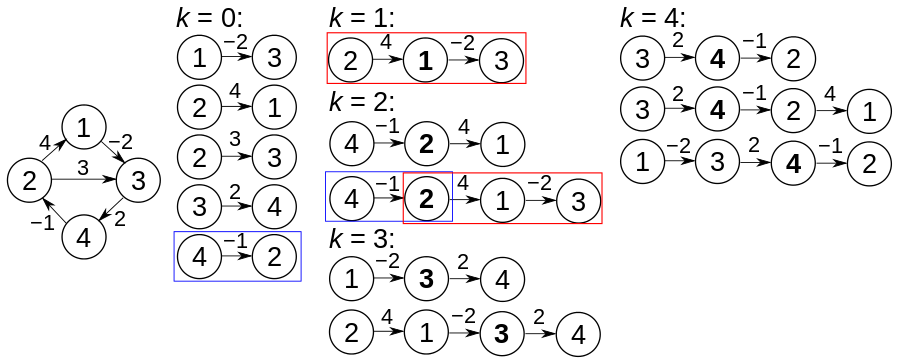
\includegraphics[width=\textwidth]{900px-Floyd-Warshall_example.svg.png}
\end{center}
\label{fig:example of Floyd-Warshall Algorithm}
\caption{An example of Floyd-Warshall Algorithm from \cite{wikipedia}.	}
\end{figure}
\end{ans}

\begin{ans}[6-23] 
(a) For all $w\in V$, check whether $d(w)$ is equal to $\dps \min_{v\rightarrow w}\{d(v)+c_{v\rightarrow w}\}$. This involves time cost $O(m+n)$.\par
(b)
Introduce new weight to the edges $c'_{v\rightarrow w }\doteq c_{v\rightarrow w}-d(v)+d(w)$. Notice
\begin{enumerate}
\item $c'_{v\rightarrow w}\geq 0$;
\item for every path $P$ beginning at $v$ and ending at $w$, denote cost of paths with respect to two weights of edges (denote two graphs by $\langle G,\{c_{\vec{e}}\}\rangle $, $\langle G,\{c'_{\vec{e}}\}\rangle $, respectively ) by $\ell(P),\ell'(P)$, then $\ell'(P)=\ell(P)-d(v)+d(w)$.
\end{enumerate}
In this case we 
\begin{enumerate}
\item run Dijkstra's algorithm on $\langle G,\{c'_{\vec{e}}\}\rangle$ with time cost $O(m\log n)$and obtain $\tilde{d}'(v)$ shortest path $v\rightarrow t'$ in $\langle G,\{c'_{\vec{e}}\}\rangle $ due to observation (1);
\item $d'(v)\leftarrow \tilde{d}'(v)+d(v)-d(t')$, which turns to be correct distances $v\rightarrow t'$ in $\langle G,\{c_{\vec{e}}\}\rangle$ due to observation (2).
\end{enumerate}
\end{ans}

\begin{ans}[HW 6.5, 6-24, Sudipto Guha]
Let the number of voters in precinct $P_i$ for the two parties be $s_i, t_i$ respectively (with
$s_i + t_i = m$). Assume party 's' has majority overall (therefore the gerrymandering can only help
party 's').

\begin{enumerate}
\item {\tt A}$[i-1,k-1,a,b]$: Is it possible to partition the precincts $P_1\ldots P_i$ such that the first part has $k$ precincts and party 's' has $a$ votes in first part and $b$ votes in second part?

Boolean value returned with $1$ true, $0$ false;
\item $${\tt A}[i,k,a,b]=\max\left\{\begin{array}{cc}
{\tt A}[i-1,k-1,a-s_i,b], & P_i\text{ is in first part};\\
{\tt A}[i-1,k,a,b-s_i], & P_i\text{ is in second part}.
\end{array}\right.$$
\item Initialization: %{\tt A}$[0,0,0,0]=1$; {\tt A}$[i,k,a,b]=1$, if $i<k$ or $k>\frac n 2$;
\item Final: $\dps \max_{\dps \frac{mn}{2}< a<\sum_{j=1}^n s_j-\frac{mn}{2}; a+b=\sum_{j=1}^n s_j} ${\tt A}$[n,\frac n 2,a, b]$;
\item Running time by evaluating \# of entities for {\tt A}: $O(n\cdot n/2\cdot mn \cdot mn)=O(m^2n^4)$.
\end{enumerate}
\end{ans}
\begin{ans}[HW 6.5, 6-24, Sudipto Guha, solution 2]
Let again the number of voters in precinct $P_i$ for the two parties be $s_i, t_i$ respectively (with
$s_i + t_i = m$). Assume again party 's' has majority overall.

Observe that $a + b =\sum^{i}_{j=1} s_j$ for any feasible partition of $P_1; \ldots Pi$. Therefore
the coordinate $b$ is superfluous.

\begin{enumerate}
\item {\tt A}$[i-1,k-1,a]$: Is it possible to partition the precincts $P_1\ldots P_i$ such that the first part has $k$ precincts and party 's' has $a$ votes in first part and $\sum_{j=1}^i s_j-a$ votes in second part?

Boolean value returned with $1$ true, $0$ false;
\item $${\tt A}[i,k,a]=\max\left\{\begin{array}{cc}
{\tt A}[i-1,k-1,a-s_i], & P_i\text{ is in first part};\\
{\tt A}[i-1,k,a], & P_i\text{ is in second part}.
\end{array}\right.$$
\item Initialization: {\tt A}$[0,0,0]=1$; {\tt A}$[i,k,a]=0$, if $i<k$ or $k>\frac n 2$;
\item Final: $\dps \max_{\dps \frac{mn}{2}< a<\sum_{j=1}^n s_j-\frac{mn}{2}} ${\tt A}$[n,\frac n 2,a]$;
\item Running time by evaluating \# of entities for {\tt A}: $O(n\cdot n/2\cdot mn )=O(mn^3)$.
\end{enumerate}

\end{ans}
\begin{ans}[6-28]
{\bf (a)} (Just the Greedy thought.)
Let $J$ be the optimal subset. By definition all jobs in $J$ can
be scheduled to meet their deadline. Now consider the problem
of scheduling to minimize the maximum lateness from class, but
consider the jobs in $J$ only. We know by the definition
of $J$ that the minimum lateness is $0$
(i.e., all jobs can be scheduled in time)by applying greedy algorithm with the ordering of their
deadline. Hence ordering 
the jobs in $J$ by the deadline generates a feasible schedule for this
set of jobs.

{\bf (b)} The problem is analogous to the subset selection problem we 
considered in section 6.1 of \cite{jon2005algorithm}: subproblems analogous to the 
ones in section 6.1 of \cite{jon2005algorithm}.  	\par 
Consider 
subproblems using a subset of jobs $\{1,\ldots,m\}$. Order the jobs by increasing deadline, and assume that 
they are numbered this way, i.e., we have that $d_1\le
\ldots \le d_n=D$. To solve the original problem we consider two cases:
either the last job $n$ is accepted or it is rejected. If job $n$ is 
rejected, then the problem reduces to the subproblem using only the 
first $n-1$ items.
Now consider the case when job $n$ is accepted. By part (a) we know 
that we may assume that job $n$ will be scheduled last. In order to 
make sure that the machine can finish job $n$ by its deadline $D$, 
all other jobs accepted by the schedule should be done by time 
$D-t_n$. We will define subproblems so that this problem is one of 
our subproblems.

For a time $0\le d \le D$ and $m=0,\ldots,n$ let 
$\opt(d,m)$ denote the the maximum subset of requests 
in the set $\{1,\ldots,m\}$
that can be satisfied by the deadline $d$. What we mean is that in this 
subproblem the machine is no longer available after time $d$, so all 
requests either have to be scheduled to be done by deadline $d$, or should
be rejected (even if the deadline $d_i$ of the job is $d_i>d$). Now we
have the following statement.
\begin{enumerate}
\item $\opt (d,m)$: maximum number of jobs amongst first $m$ jobs in first $d$ time units;
\item final: $\opt (d,n)$;
\item $$\opt (d,m)=\max\left\{\begin{array}{c}\opt(m-1,d),\\ \opt(m-1,d-t_m)+1\}\end{array}\right.$$
that is, selecting between whether or not job $m$ is in the optimal solution $\opt (d,m)$;
\item 
\item 
\end{enumerate}
\begin{State} \label{jobs-rec}
\begin{itemize}
\item 
\end{itemize}
\end{State}
This suggests the following code.
\begin{quote}
\begin{code}
{\tt Select-Jobs(n,D)}:\\
\begin{enumerate}
\item  Array $M[0\ldots n,0 \ldots D]$
\item  Array $S[0\ldots n,0 \ldots D]$
\item   For $d=0,\ldots,D$
	\begin{enumerate}
\item     $M[0,d]=0$
\item     $S[0,d]=\phi$
	\end{enumerate}
\item    Endfor
\item    For $m=1,\ldots,n$
\item      For $d=0,\ldots,D$
\begin{enumerate}
\item        If $M[m-1,d]>M[m-1,d-t_m]+1$ then \\$M[m,d]=M[m-1,d]$, $S[m,d]=S[m-1,d]$;
\item        Else \\$M[m,d]=M[m-1,d-t_m]+1$, $S[m,d]=S[m-1,d-t_m] \cup\{m\}$.
\item       Endif
\end{enumerate}
\item     Endfor
\item   Endfor
\item   Return $M[n,D]$ and $S[n,D]$
   \end{enumerate}
\end{code}
\end{quote}

The correctness follows immediately from the statement 
\ref{jobs-rec}.  The running time of $O(n^2D)$ is also immediate 
from the for loops in the problem, there are two nested  {\tt for}
loops for for $m$ and one for $d$. This means that the internal part
of the loop gets invoked $O(nD)$ time. 
The internal part of this {\tt for} loop
takes $O(n)$ time, as we explicitly maintain the optimal solutions. 
The running time can be improved to $O(nD)$ by not maintaining the
$S$ array, and only recovering the solution later, once the values
are known. 

\end{ans}

\begin{ques}[Fall 2014-I, 25 points]
 A subsequence is defined to be palindromic if it is the same when it
is read left-to-right or right-to-left. A sequence can have many palindromic subsequences. For
example
$$a; b; a; f; a; b; a; c; d; e; d; c$$
Has several such subsequences $aba; aa; baab; cdedc$, etc. Give an efficient (as low running time as
possible) algorithm to find the longest palindromic subsequence of a sequence $a1; a2;\ldots ;an$. For
full credit give an $O(n^2)$ time algorithm. A subsequence need not be a substring (contiguous) as the example shows.
\end{ques}


\begin{ans}[1, SUDIPTO GUHA]
\begin{enumerate}
\item $LCS[i; j]$: (length of the) longest common subsequence of 
$X_1; \ldots ;X_i$ and $Y_1;\ldots; Y_j $.
\item Final answer is $LCS[|X|; |Y |]$;
\item $LCS[i; j] = \max \left\{
\begin{array}{cc}
LCS[i -1; j]\\
LCS[i; j -1]\\
1 + LCS[i -1; j -1] &\text{(provided }X_i = Y_j, \\
&\text{otherwise this option does not exist)}
\end{array}
\right.
$
\item 
$LCS[i; 0] = LCS[0; j] = 0 ,\forall i, j$;
\item The size of the table is $O(n^2)$
and each entry is updated in $O(1)$ time.
\end{enumerate}
\end{ans}


\begin{ans}[2, SUDIPTO GUHA]
\begin{enumerate}
\item $PAL[i; j]$: (length of the) longest palindromic sequence.
\item Final answer is $PAL[1;n]$;
\item $LCS[i; j] = \max \left\{
\begin{array}{cc}
PAL[i +1; j]\\
PAL[i; j -1]\\
1 + PAL[i +1; j -1] &\text{(provided }X_i = Y_j, \\
&\text{otherwise this option does not exist)}
\end{array}
\right.
$
\item $PAL[i; j] = 0, PAL[i;i]=1,\forall i> j$;
\item running time $O(n^2)$.
\end{enumerate}
\end{ans}


\begin{ques}[2015 midterm 2] Given $n$ numbers $x_1,\ldots,x_n$, the numbers $x_{i_1},x_{i_2},\ldots,x_{i_k}$ define a sub-sequence if $1\leq i_1<i_2<\ldots<i_k\leq n$. Length of the sub-sequence is $k$. For example given $1.1,-2,0,-6,17.2,13$ the numbers $1.1, 17.2, 13$ define a sub-sequence of length $3$.
\begin{enumerate}
\item Given $x_1,\ldots, x_n$ as above, give a polynomial time DP algorithm that finds the length of the maximum length \textit{increasing} sub-sequence. A sub-sequence above is of length $3$, either $-2,0,17.2$ or $-2,0,13$. Just finding the length will suffice.
\item Define a sub-sequence $x_{i_1},x_{i_2},\ldots,x_{i_k}$ to be "maybe increasing" if $x_{i_a}-7<x_{i_b}$ for any $1\leq i_a<i_n\leq k$. That is, the sub-sequence never decreases by more than $7$. for example the sub-sequence $-2,0,-6,17.2,13$ is "maybe increasing" but the entire sequence is not. given $x_1,\ldots,x_n$ as above. Given $x_1,\ldots,x_n$ as above, find the length of the maximum length "maybe increasing" sub-sequence.

\item Define a sub-sequence $x_{i_1},\ldots,x_{i_k}$ to be "surely increasing" if $x_{i_1}+7<x_{i_2},x_{i_2}+7<x_{i_3}$, etc., that is, the numbers are not only increasing but also differ by at least $7$. For example the sub-Given $x_1,\ldots,x_n$ as above, find the length of the maximum length "surely increasing" sub-sequence.
\end{enumerate}
\end{ques}
\begin{ans}[2015 midterm 2]
\begin{enumerate}
\item 
\begin{enumerate}
\item Define $x_{n+1}=\infty,\forall x\in\Reals,x<x_{n+1}=\infty$; define
{\tt opt}$[j,k]$: max length of "maybe increasing" sub-sequence of $\{x_1,x_2,\ldots,x_j\}$ such that every element is smaller than $x_k$ ($j=1,2,\ldots, n,k=j+1j+2,\ldots,n+1$;
\item {\tt opt}$[j,k]\leftarrow\max\left\{
\begin{array}{rl}
1+{\tt opt}[j-1,j], & \text{the option is available iff } x_j<x_k; \\
{\tt opt}[j-1,k] & x_j \text{ is not selected}.
\end{array}
\right.$
\item Final {\tt opt}$[n,n+1]$;
\item Initialization: {\tt opt}$[1,k]=\left\{
\begin{array}{rl}
1, & x_1<x_k+7;\\
0,&\text{otherwise}
\end{array}
\right., k=2,\ldots, n+1$;
\item Running time $O(n^2)$.
\end{enumerate}
\item 
\begin{enumerate}
\item Define $x_{n+1}=\infty,\forall x\in\Reals,x<x_{n+1}=\infty,\infty+7=\infty$; define
{\tt opt}$[j,k]$: max length of "maybe increasing" sub-sequence of $\{x_1,x_2,\ldots,x_j\}$ such that every element is smaller than $x_k$ ($j=1,2,\ldots, n,k=j+1,j+2,\ldots,n+1$;
\item {\tt opt}$[j,k]\leftarrow\max\left\{
\begin{array}{rl}
1+{\tt opt}[j-1,j], & \text{the option is available iff } x_j<x_k; \\
{\tt opt}[j-1,k] & x_j \text{ is not selected}.
\end{array}
\right.$
\item Final {\tt opt}$[n,n+1]$;
\item Initialization: {\tt opt}$[1,k]=\left\{
\begin{array}{rl}
1, & x_1<x_k+7;\\
0,&\text{otherwise}
\end{array}
\right., k=2,\ldots, n+1$;
\item Running time $O(n^2)$.
\end{enumerate}
\item same as 1 with running time $O(n^2)$.
\end{enumerate}
\end{ans}

\begin{ques} 
You are given an array $A[1],\ldots,A[n]$ which contain both negative and
positive values. Assume $A[0] = A[n + 1] = 0$.
\begin{enumerate} 
\item \textbf{(10 points)} Find an interval $[i, j]$ such that
$\sum_{t=i}^j A[t]$ is maximized. An $O(n^2)$ solution will not get any credit.
\item \textbf{(10 points)} Find two intervals $[i,j]$ and $[k,l]$ where $i \leq j < k\leq l$ such that
$\sum^j_{t=i} A[t]+
\sum^j_{t=k} A[t]$
is maximized. An $O(n^4)$ solution will not get any credit.
\end{enumerate}
More credit will be provided to a solution which is more efficient. 
\end{ques}
\begin{ans}
\begin{enumerate}
\item 
\begin{enumerate}
\item $B[j]=\max $ sum of any interval of $1,\ldots,j$ ending in $j$;
\item $B[j] \leftarrow \max\{B[j - 1] + A[j], A[j]\}$,

 since if we
include $j-1$ in that interval then we should include the largest interval ending in $j-1$ -- adding $A[j]$ with $B[j-1]$, sum of any interval of $1,\ldots, j-1$ ending in $j-1$;
\item Final $B[n]$;
\item Initialization: $B[0]=0$;
\item Running time $O(n)$.
\end{enumerate}
\item 
\begin{enumerate}
\item $C[i]=\max$ sum of any interval starting from $i$;

$C'[i]=\max_{s\geq i} C[s]$ which means the largest interval sum starting after $i$.  This can be computed in $O(n)$ time;
\item $C[i]\leftarrow \max\{ B[i+1]+A[i], A[i] \}$\footnote{That is what Sudipto Guha says, "\textcolor{red}{(switching $i$ for $j$ and $n+1$ for $0$ and $i+1$ for $j -1$)}".};
\item Final $\max_j \{B[j] + C'[j + 1]\}$;
\item Intialization;
\item Running time $O(n)$.
\end{enumerate}
\end{enumerate}
Here we finish.
\end{ans}

\section{Ch7 Network flow}
\begin{ques}[HW5, 7-10]
Suppose you are given a directed graph $G = (V,E)$, with
$c_e>0,\forall e\in E$.
a designated source $s \in V$, and a designated sink $t \in V$.
You are also given a maximum $s$-$t$ flow in $G$,
defined by a flow value $f_e$ on each edge $e$.
The flow $\{f_e\}$ is {\em acyclic}: there is
no cycle in $G$ on which all edges carry positive flow.
\par 
Now, suppose we pick a specific edge $\vec{e}^* \in E$
and reduce its capacity by $1$ unit.
Show how to find a maximum flow in the resulting
capacitated graph in time $O(m)$,
where $m$ is the number of edges in $G$.
\end{ques}

\begin{ans}[HW5, 7-10] Denote capacity of directed edge $\vec{e} \in E_2$ by $c_{\vec{e}}$ in the last residual graph $G_2=\langle V,E_2\rangle $ with $\{c_{\vec{e}}\in \mathcal{N}_{\geq 0}:\vec{e}\in E_2\}$. Denote  $\vec{e}^*=(u,w)$.  
\begin{enumerate}
\item If $c_{(w,u)}=0$, then the maximum flow does not change since $\vec{e}^*$ must have not been take advantage of to ship any flow to form the maximum flow;
\item Else, 
\begin{enumerate}
\item use DFS to find a $u\rightarrow s$ path $P_1=uv_{k-1}v_{k-2}\ldots v_1s$ and a $t\rightarrow w$ path $P_2=tv_{l-1}v_{l-2}\ldots v_{k+2}w$ in the residual graph with $c_{(v_{j+1},v_j)}>0$ ($s=v_0,u=v_k,w=v_{k+1},t=v_l$) . These run with $O(m+n)$ time;
\item Update capacities in the following way:
\begin{enumerate}
\item $c_{(v_{k},v_{k+1})}'\leftarrow c_{(v_{k},v_{k+1})}, c_{(v_{k+1},v_k)}'\leftarrow c_{(v_{k+1},v_k)}-1$;
\item $c_{(v_{j},v_{j+1})}'\leftarrow c_{(v_{j},v_{j+1})}+1,, c_{(v_{j+1},v_j)}'\leftarrow c_{(v_{j+1},v_j)}-1$, $j=0,1,\ldots,l-1,j\neq k$.
\end{enumerate}
Now we construct new $\{c_{\vec{e}}\in \mathcal{N}_{\geq 0}':\vec{e}\in E_2\}$ for $G_2=\langle V,E_2\rangle $. This runs with time $O(m)$.
\end{enumerate}
\item Use DFS to search whether there is a positive $s\rightarrow t$ flow. This runs with $O(m+n)$ time. If exists, the value of maximum flow does not change (although the flow does change); if not, the value maximum flow is reduced by $1$ unit.
\end{enumerate}\par 
Total running time is at most $O(m+n)$.\par 
\textbf{Correctness}:
\end{ans}
%\begin{rem} Part 1 and part 2 in the answer can actually be written in a unified form:
%\end{rem}
\begin{rem} How about add $1$ unit to capacity of the  	specific edge $e^*\in E$?
\end{rem}
\begin{ans}[refers in \cite{mit2004springcs}] Add the new flow to the residual flow graph in $O(m)$ time. Perform a tree traversal from the source node to detect whether a path now exists to the sink. If so, augment along that path and increase the maximum flow by one. If exists, augment along that path and increase the maximum flow by one.
\par
The running time is $O(n)$.
\par
\textbf{Correctness}:	
\end{ans}
\begin{ques}[HW5, 7-12]
Consider the following problem.
You are given a flow network with unit-capacity edges:
it consists of a directed graph $G = (V,E)$, a source $s \in V$,
and a sink $t \in V$; and $c_e = 1$ for every $e \in E$.
You are also given a parameter $k$.\par

The goal is delete $k$ edges so as to reduce
the maxmimum $s$-$t$ flow in $G$ by as much as possible.
In other words, you should find a set of edges $F \subseteq E$
so that $|F| = k$ and
the maximum $s$-$t$ flow in $G' = (V,E - F)$ is as
small as possible subject to this.\par 

Give a polynomial-time algorithm to solve this problem.
\end{ques}
\begin{ans}[HW5, 7-12, refers to \cite{solcornell}]
If the minimum $s$-$t$ cut has size $\leq k$ (since the flow network with unit-capacity edges),
then we can reduce the flow to $0$.

Otherwise, let $f > k$ be the value of the maximum $s$-$t$ flow.
We identify a minimum $s$-$t$ cut $(A,B)$,
and delete $k$ of the edges out of $A$.
The resulting subgraph has a maximum flow value of at most $f - k$ (by (7.9) in \cite{jon2005algorithm}).
\begin{State}[\textbf{Claim}]
For any set of edges $F$ of size $k$,
the subgraph $G' = (V,E - F)$ has an $s$-$t$ flow of value at least $f - k$.
\end{State}
\begin{proof}
Indeed, consider any cut $(A,B)$ of $G'$.
There are at least $f$ edges out of $A$ in $G$,
and at most $k$ have been deleted,
so there are at least $f - k$ edges out of $A$ in $G'$.
Thus, the minimum cut in $G'$ has value at least $f - k$,
and so there is a flow of at least this value.
\end{proof}
\end{ans}
\begin{rem}
What if not "with unit-capacity edges"?
\end{rem}
\begin{ques}[HW5, 7-14]

We define the {\em escape problem} as
follows:

  We are given a directed graph $G = (V,E)$ (picture a
network of roads); a certain collection of nodes $X \subset V$
are designated as {\em populated nodes}, and a certain
other collection $S \subset V$ are designated as {\em safe nodes}.
(Assume that $X$ and $S$ are disjoint.)
In case of an emergency, we want evacuation routes
from the populated nodes to the safe nodes.
A set of evacuation routes is defined as a set
of paths in $G$ so that 
\begin{enumerate}
\item[(i)] each node in $X$ is the tail of one path, 
\item[(ii)] the last node on each path lies in $S$, and
\item[(iii)] the paths do not share any edges.
\end{enumerate} 
Such a set of paths gives a way for the
occupants of the populated nodes to ``escape'' to $S$,
without overly congesting any edge in $G$.

\begin{enumerate}
\item[(a)]  Given $G$, $X$, and $S$, show how to decide in
polynomial time whether such a set of evacuation routes exists.
\item[(b)]  Suppose we have exactly the same problem as in (a),
but we want to enforce an even stronger version of
the ``no congestion'' condition (iii).
Thus, we change (iii) to say
``the paths do not share any {\em nodes}.''

With this new condition, show how to decide in
polynomial time whether such a set of evacuation routes exists.

Also, provide an example with a given $G$, $X$, and $S$, in which
the answer is ``yes'' to the question in (a) but ``no''
to the question in (b).
\end{enumerate}
\end{ques}
\begin{ans}[HW5, 7-14]
(a) Redistribute nodes in $X$ left side and nodes in $S$ right side as shown in figure \ref{fig:7-14-a construction of graph}. Add source $s$, sink $t$ to $V$ and add directed edges to $E$.  Assign each edge with capacity $1$ -- this is important to avoid paths sharing edges. In all, denote 
$$E'\leftarrow \{(s,v):v\in S\}\cup \{(u,t):u\in X \}\cup E, V'\leftarrow V\cup \{s,t\},$$
and we actually construct a new graph $G'=\langle V',E'\rangle$ (with capacity on each edge) on which can apply algoritm to find maximum flow.\par
If apply generic Preflow--Push Maximum--flow Algorithm in section 7.4 of \cite{jon2005algorithm}, by statement (7.33) of \cite{jon2005algorithm} we can obtain it with running time $O\left((m+n)n^2)\right)=O(mn^2+n^3)$; in the version where we always select the node at maximum height runs in $O(n^3)$ time.
\par
A set of evacuation routes exists if and only if value of maximum flow is $|X|$.
\begin{figure}
\begin{center}
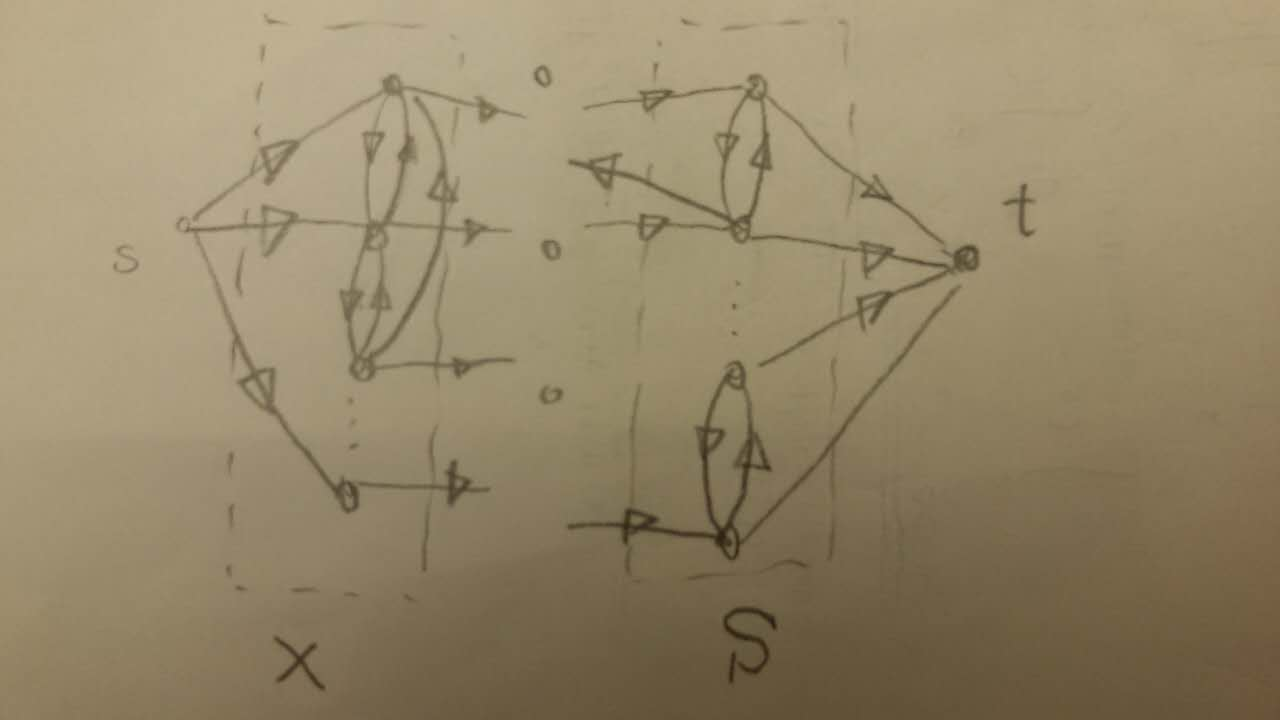
\includegraphics[width=\textwidth]{7_14_a.jpg}
\end{center}
\caption{Construction of graph}
\label{fig:7-14-a construction of graph}
\end{figure}
\par 
(b) 

\begin{figure}
\begin{center}
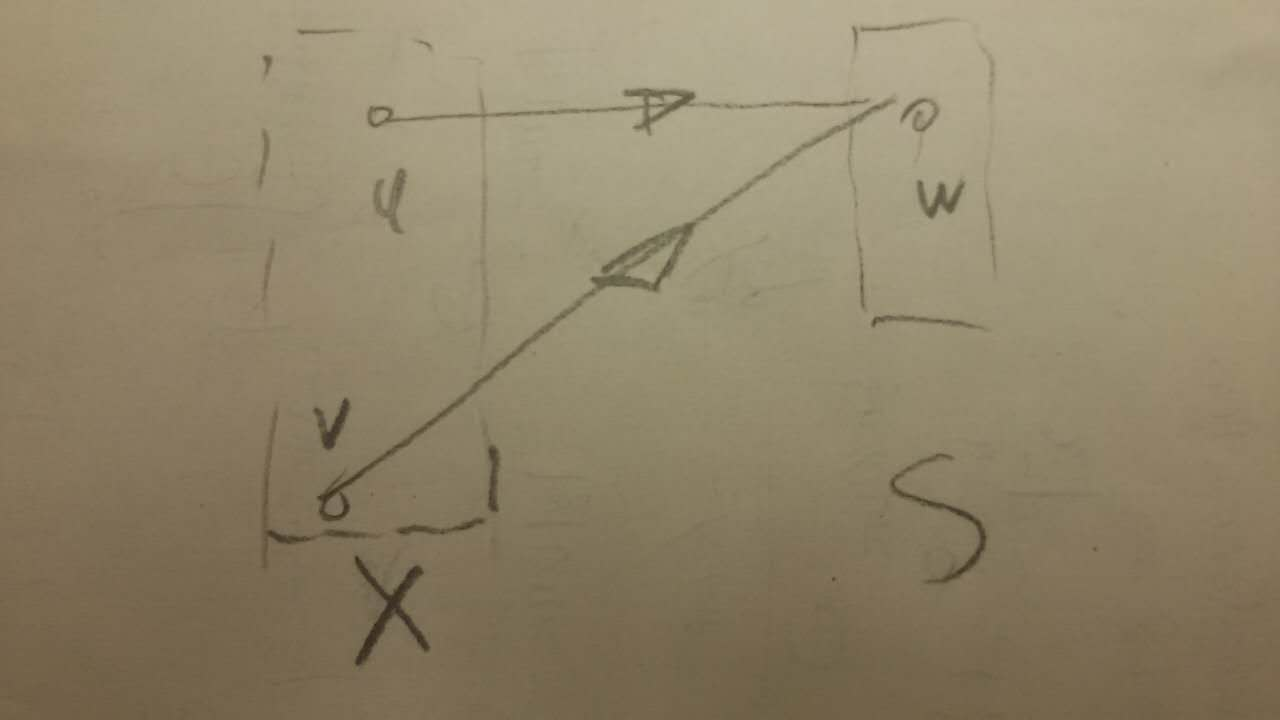
\includegraphics[width=\textwidth]{7_14_b.jpg}
\end{center}
\caption{An example showing (a) "yes" but (b) "no".}
\label{fig:7-14-b an example}
\end{figure}
\end{ans}
\begin{ans}[7-14, Sudipto Guha]
(a) Running time is $O(|X|(m+n))$ by Ford-Fulkerson algorithm in section 7.1 of \cite{jon2005algorithm}.
\par 
(b)split every vertex $v\in V$ into $2$ pieces $v_{in},v_{out}$ and denote:
 $$V''\leftarrow \{v_{in},v_{out}:v\in V\}\cup \{s_{out},t_{in}\}, E''\leftarrow \{(u_{out},u_{in}:(u,v)\in E'\},G''\leftarrow \langle V'',E''\rangle,$$
Compute the maxflow on $G''$ which provides us the escape routes.
\end{ans}
\begin{ques}[HW5, 7-17]
You've been called in to help some network administrators diagnose the extent of a failure in their network. The network is designed to carry traffic from a designated source node $s$ to a designated target node $t$, so we will model it as a directed graph $G = (V,E)$, in which the capacity of each edge is $1$, and in which each node lies on at least one path from $s$ to $t$.
\par
Now, when everything is running smoothly in the network, the maximum $s-t$ flow in $G$ has value $k$. However, the current situation -- and the reason you're here -- is that an attacker has destroyed some of the edges in the network, so that there is now no path from $s$ to $t$ using the remaining (surviving) edges. For reasons that we won't go into here, they believe the attacker has destroyed only $k$ edges, the minimum number needed to separate $s$ from $t$ (i.e. the size of a minimum $s-t$ cut); and we'll assume they're correct in believing this.
\par
The network administrators are running a monitoring tool on node $s$, which has the following behavior: if you issue the command ping($v$), for a given node $v$, it will tell you whether there is currently a path from $s$ to $v$. (So ping($t$) reports that no path currently exists; on the other hand, ping($s$) always reports a path from $s$ to itself.) Since it's not practical to go out and inspect every edge of the network, they'd like to determine the extent of the failure using this monitoring tool, through judicious use of the ping command.
\par
So here's the problem you face: give an algorithm that issues a sequence of ping commands to various nodes in the network, and then reports the full set of nodes that are not currently reachable from $s$. You could do this by pinging every node in the network, of course, but you'd like to do it using many fewer pings (given the assumption that only $k$ edges have been deleted). In issuing this sequence, your algorithm is allowed to decide which node to ping next based on the outcome of earlier ping operations.
\par
Give an algorithm that accomplishes this task using only $O(k \log n)$ pings. 
\end{ques}
\begin{ans}[HW 5, 7-17, Sudipto Guha]
Observe that if the mincut in the graph was unique then we already knew which edges were cut! So there are multiple min-cuts and the goal is to find which mincut has been destroyed.

\begin{enumerate}
\item Run Ford-Fulkerson to find a maxflow of $k$; we then perform a flow decomposition and
get $k$ edge disjoint paths from $s$ to $t$. Each of these steps require $O(mk)$ time.
\begin{claim}
Every cut contains one of the edges from each of these paths.
\end{claim}
\begin{proof}
Suppose not, it is not separating
$s$ and $t$. Therefore every mincut has exactly one edge from each of the paths -- otherwise that cut
will have more than $k$ edges and will not be a mincut.
\end{proof}

Therefore the adversary has destroyed exactly one edge on each of the paths we found. We can
now perform binary search to find the specific edge which has been cut.
\item $O(\log n)$ pings on every paths since each path is of length at most $n$.
\end{enumerate}
We need $O(k \log n)$ pings.
\end{ans}

\begin{ans}[HW 6.5, 7-22] Bipartite graph whether or not with perfect matching.
\end{ans}

\begin{ques}[HW6, 7-23] Suppose you're looking at a flow network $G$
with source $s$ and sink $t$, and
you want to be able to express something like the following
intuitive notion: some nodes are clearly on the ``source side''
of the main bottlenecks; some nodes are clearly on the ``sink side''
of the main bottlenecks; and some nodes are in the middle.
However, $G$ can have many minimum cuts, so we have
to be careful in how we try making this idea precise.

Here's one way to divide the nodes of $G$ into three
categories of this sort.
\begin{itemize}
\item We say a node $v$ is {\em upstream} if for all minimum $s$-$t$ cuts $(A,B)$, we have $v \in A$ --- that is, $v$ lies on the source side of every minimum cut. \item We say a node $v$ is {\em downstream} if for all min $s$-$t$ cuts $(A,B)$, we have $v \in B$ --- that is, $v$ lies on the sink side of every min cut. 

\item We say a node $v$ is {\em central} if it is neither upstream nor downstream; there is at least one min $s$-$t$ cut $(A,B)$ for which $v \in A$, and at least one min $s$-$t$ cut $(A',B')$ for which $v \in B'$.
\end{itemize}

Give an algorithm that takes a flow network $G$, and
classifies each of its nodes as being upstream, downstream, or central.
The running time of your algorithm should be within in a constant
factor of the time required to compute a {\em single} max flow.
 
\end{ques}
\begin{lem} Given a max flow $f$ and a min cut $(A,B)$ for a $s-t$ flow problem. Two of which might not be required to have any correspondence\footnote{In other word, $(A,B)$ is not necessarily obtained from $G_f$.}. Then no edge $\in G_{f}$ can go from $A$ to $B$.
\end{lem}
\begin{proof}
Suppose not, then (7.8) of \cite{jon2005algorithm} implies $\nu(f)<c(A,B)$ where
$$\nu(f)\doteq \text{value of flow }f, c(A,B)\doteq \sum_{e\text{ out of }A}c_e.$$
A contradiction by (7.13) of \cite{jon2005algorithm}.
\end{proof}
\begin{ans}[HW6, 7-23, refers to \cite{solcornell}] 
Consider the cut $(A^*,B^*)$ found by performing
BFS on $G_f$\footnote{Residual graph of flow $f$.} at the end of 
any $\max$ flow algorithm.
\begin{State}[Claim 1]
A node $v$ is upstream iff $v \in A^*$.
\end{State}
\begin{proof}
$\Rightarrow)$ If $v$ is upstream, then $v\in A^*$ (otherwise, it lies on the sink-side of the minimum cut $(A^*,B^*)$); 

$\Leftarrow) $ Suppose not, that is, $\exists v \in A^*$ were not upstream.
Then $\exists (A',B')$ (a minimum cut) with $v \in B'$:
\begin{enumerate}
\item $v \in A^*\Rightarrow \exists P_{s\rightarrow v}\in G_{f^*}$;
\item $v \in B'\Rightarrow \exists $ edge $(u,w)\in P_{s\rightarrow v}$ with
$u \in A'$ and $w \in B'$.
\end{enumerate}
A contradiction since no edge $\in G_{f^*}$ can go from the source side to the sink side
of any minimum cut by lemma.
\end{proof}
A completely symmetric argument shows the following.
Let $B_*$ denote the nodes that can reach $t$ in $G_f$,
and let $A_* = V - B_*$.
Then $(A_*, B_*)$ is a minimum cut. Then
\begin{State}[Claim 2]
A node $w$ is downstream iff $w \in B_*$.
\end{State}
\begin{proof}
$\Rightarrow)$ If $w$ is downstream, then $w\in B_*$ (otherwise, it lies on the source-side of the minimum cut $(A_*,B_*)$); 

$\Leftarrow) $ Suppose $w \in B_*$ were not downstream.
Then there would be a minimum cut $(A',B')$ with $w \in A'$:
\begin{enumerate}
\item $w \in B_*\Rightarrow \exists P_{w\rightarrow t}\in G_{f_*}$;
\item $w \in A'\Rightarrow \exists $ edge $(u,v)\in P_{w\rightarrow t}$ with
$u \in A'$ and $w \in B'$.
\end{enumerate}
A contradiction since no edge in the
residual graph can go from the source side to the sink side of any minimum cut by lemma.
\end{proof}

Thus, our algorithm is to compute a maximum flow $f$, 
build construct residual graph $G_f$, and use BFS to find the
sets $A^*$ and $B_*$.
These are the upstream and downstream nodes respectively;
the remaining nodes are central.
\end{ans}


\begin{ans}[HW 6, 7-23, Sudipto Guha, Yezheng Li]
Compute a max flow $f$ (then fixed)\footnote{Using any algorithm.}
,$G_f$. Now consider 
\begin{enumerate}
\item $S\doteq\{v\in V:\exists \text{ path }P_{s\rightarrow v}\in G_f\}$, the set of all nodes reachable from $s$ with capacity $>0$ edges in the residual graph. 
\item $T\doteq\{w\in V:\exists \text{ path }P_{w\rightarrow t}\in G_f\}$, the set of all nodes which can reach $t$ with capacity $>0$ edges in the residual graph. 
\end{enumerate}
where notice
\begin{claim} Both $(S,V-S)$, $(V-T,T)$ are min cuts of $G$.
\end{claim}
\begin{proof}
In $G_f$, no positive weighted edge $V-S\to S$ or $T\to V-T$.
\end{proof}
Then
\begin{claim}[Yezheng Li]$S\subset A',T\subset B'$ for any minimum cut $(A',B')$.
\end{claim}
\begin{proof}[Yezheng Li]
\begin{enumerate}
\item Speaking of $S\subset A'$. Suppose not, that is, $\exists v\in S\setminus A'\Rightarrow v\in S\cap B'$. Then
\begin{enumerate}
\item $v \in S\Rightarrow \exists s\rightarrow v$ path $P_{s\rightarrow v}\in G_f$.

\item $v \in B'\Rightarrow \exists (u,w)\in P_{s\rightarrow v}$ with $u \in A', w \in B'$.
\end{enumerate}
 A contradiction since no edge $\in G_{f}$ can go from the source side to the sink side of any minimum cut by lemma;
\item Likewise, speaking of $T\subset B'$. Suppose not, that is, $\exists w\in T\setminus B'\Rightarrow w\in T\cap A'$. Then
\begin{enumerate}
\item $w \in T\Rightarrow \exists w\rightarrow t$ path $P_{w\rightarrow t}\in G_f$.

\item $w \in A'\Rightarrow \exists (u,v)\in P_{w\rightarrow t}$ with $u \in A', v \in B'$.
\end{enumerate}
 A contradiction by lemma again.
\end{enumerate}
To conclude, the proof is finished.
\end{proof}
\begin{claim}[Sudipto Guha]
Every node in $S$ is upstream, every node in $T$ is downstream. The remaining nodes are central.
\end{claim}
\begin{proof}[Yezheng Li] 
By \textbf{Claim 1} we know "every node in $S$ is upstream" and "every node in $T$ is downstream".

Furthermore,
\begin{enumerate}
\item If $v$ is upstream, then 	$v\in S$.
\begin{proof}
Suppose not. $\exists v\notin S$ but is upstream. $v\notin S$ means no $s\rightarrow v$ path $\in G_f$,  $\Rightarrow$ $(S,V-S)$ is a min cut of $G$ such that $v\in V-S$ $\Rightarrow$ A contradiction by   definition of "upstream".
\end{proof}
\item Analogously, if $w$ is downstream, then $w\in T$.
\begin{proof}
Suppose not. $\exists w\notin S$ but is downstream. $w\notin T$ means no $w\rightarrow t$ path $\in G_f$, $\Rightarrow$ $(V-T,T)$ is a min cut of $G$ such that $w\in V-T$ $\Rightarrow$ A contradiction by definition of "downstream".
\end{proof}

\end{enumerate}
To conclude,$S$ is the set of all upstream nodes and $T$ is the set of all downstream nodes.
\end{proof}
\end{ans}

\begin{ans}[7-24] By 7-23, one can just check whether or not $S=A,T=B$ to answer the question.
\end{ans}

\begin{ans}[HW 6.5, 7-27] Create a bipartite graph where $L=\{D_1,\ldots,D_d\}$ corresponds to the days and $R=\{P_1,\ldots,P_k\}$ corresponds
to the people. If person $j$ is present in $S_i$ (the set of people going on day i) then draw a directed
arc from $D_i \rightarrow P_j$. Now add a source $s$ which connects to each $P_i \in L$ with capacity $1$ (meaning we need 1 driver for that day) and a sink t which connects to each $j$ with capacity $\lceil \triangle_j\rceil$.

Observe that the fractional fair schedule defines a fractional flow of capacity $d$ from $s$ to $t$ -- here 1 unit of flow is sent from $s$ to each $i$ and the flow on the $i\rightarrow j$ edge is $\frac{1}{|S_j|}$. The total flow
arriving at $j$ is $\triangle_j\leq \lceil \triangle_j\rceil =c_{j \rightarrow t}$. 
\begin{State}[Claim 1] 
Max flow is $d$.
\end{State}
\begin{proof}
According to fractional fair schedule, max flow is at least $d$. But there is a cut $\langle \{s\}, V-\{s\}\rangle$ of capacity  $d$. Therefore, max flow is $d$.
\end{proof} 
We can now use Ford Fulkerson to find the max flow (it will be an integral flow, in time $O(kd^2)$ because the total number of edges is at most $kd$. The flow can be decomposed into d paths
each carrying one unit flow in time $O(kd^2)$. The flow paths through $j$ correspond to the days $j$ is
driving. Observe that the schedule is fair by construction. Note this proves the existence, part (a)
and the construction, part (b) simultaneously.
\end{ans}

\begin{ques}[HW6, 7-31] Some of your friends are interning at the small high-tech company WebExodus.
A running joke among the employees there is that the back room
has less space devoted to high-end servers than it does to
empty boxes of computer equipment, piled up in case something
needs to be shipped back to the supplier for maintainence.

A few days ago, a large shipment of computer monitors
arrived, each in its own large box;
and since there are many different kinds of monitors
in the shipment, the boxes do not all have the same dimensions.
A bunch of people spent some time in the morning
trying to figure out how to store all these things,
realizing of course that less space would be taken up if
some of the boxes could be {\em nested} inside others.

Suppose each box $i$ is a rectangular parallelepiped
with side lengths equal to $(i_1, i_2, i_3)$;
and suppose each side length is strictly between half a meter and one meter.
Geometrically, you know what it means for one box
to nest inside another --- it's possible if you can rotate the
smaller so that it fits inside the larger in each dimension.
Formally, we can say that box $i$ with dimensions $(i_1, i_2, i_3)$
{\em nests} inside box $j$ with dimensions $(j_1, j_2, j_3)$ if
there is a permutation $a, b, c$ of the dimensions $\{1, 2, 3\}$
so that $i_a < j_1$, and $i_b < j_2$, and $i_c < j_3$.
Of course, nesting is recursive --- if $i$ nests in $j$,
and $j$ nests in $k$, then by putting $i$ inside $j$ inside $k$,
only box $k$ is visible.
%%And so on for larger sequences of boxes \ldots\
We say that a {\em nesting arrangement} for a set
of $n$ boxes is a sequence of operations in which
a box $i$ is put inside another box $j$ in which it nests;
and if there were already boxes nested inside $i$,
then these end up inside $j$ as well.
(Also notice the following:
since the side lengths of $i$ are more than half a meter each,
and since the side lengths of $j$ are less than a meter each,
box $i$ will take up more than half of each dimension of $j$,
and so after $i$ is put inside $j$, nothing else can be put inside $j$.)
We say that a box $k$ is {\em visible} in a nesting
arrangement if the sequence of operations does not
result in its ever being put inside another box.

So this is the problem faced by the people at WebExodus:
Since only the visible boxes are taking up any space,
how should a nesting arrangement be chosen
so as to minimize the {\em number} of visible boxes?

Give a polynomial-time algorithm to solve this problem.

\smallskip
{\bf Example.} Suppose there are three boxes with dimensions
$(.6, .6, .6)$, $(.75, .75, .75)$, and $(.9, .7, .7)$.
Then the first box can be put into either of the second
or third boxes;
but in any nesting arrangement, both the
second and third boxes will be visible.
So the minimum possible number of visible boxes is two,
and one solution that achieves this is to
nest the first box inside the second.

\end{ques}



\begin{ans}[HW 6, 7-31, refers to \cite{solcornell} and section 7.9 of \cite{jon2005algorithm}] Reduce the given problem to a max flow problem
where units of flow correspond to sets of boxes nested
inside one visible box.
We construct the following directed graph $G=\langle V,E\rangle$:
\begin{itemize}
\item about nodes $V$:
\begin{itemize}
\item For each box $i$, two nodes $\{u_i,v_i\}\subset V$; 
\item A source node $s\in V$, corresponding to the back room where
  boxes are stored; \par 
  a sink node $t\in V$, corresponding to nothing inside
  empty boxes.
\end{itemize}
\item about edges $E$:
\begin{itemize}
\item between $u_i,v_i$ that corresponds to this box, an edge $(u_i,v_i)\in E$ with
since each box is exactly in one set of boxes nested one in another.;
\item   $\exists$ an edge $(v_i,u_j)\in E$ for each $i$ and $j$ so that box $j$ can nest inside box $i$;
\item Edges $\{(s,u_i),i=1,2,\ldots, n\}\subset E$ since any box can be visible;
\item Edges $\{(v_j,t),j=1,2,\ldots, n\}\subset E$ since any box can be empty.
\end{itemize}
Each edge $u\rightarrow v$ has capacity $c_{u\rightarrow v}=1$ such that $0\leq f_{u\rightarrow v}\leq c_{u\rightarrow v}=1$.
\item about demands:
\begin{itemize}
\item $d_{u_i}=d_{v_i}=0$;
\item $d_s=-k,d_t=k$.
\end{itemize}
\end{itemize}
We claim the following:
\begin{State}[Claim]
{\em There is a nesting arrangement with $k$ visible boxes if and only of
  there is a feasible circulation in $G$ with demand $-k$ in the source node
  $s$ and demand $k$ in the sink $t$.
}
\end{State}

\begin{proof}
$\Rightarrow )$ Suppose there is a nesting arrangement with $k$ visible boxes.
Each sequence of nested boxes inside one visible box $i_1$, $i_2$, \dots, $i_n$
defines a path from $s$ to $t$:
$$(s,u_{i_1},v_{i_1},u_{i_2},v_{i_2},\dots,u_{i_n},v_{i_n},t)$$
Therefore we have $k$ paths from $s$ to $t$.
The circulation corresponding to all these paths satisfy all demands,
capacity and lower bound.

$\Leftarrow )$  consider a feasible circulation (with integer flow values) in our network.
There are exactly $k$ edges going to $t$ that carries one unit of flow.
Consider one of such edges $(v_i,t)$.
We know that $(u_i,v_i)$ has one unit of flow.
Therefore, there is a unique edge into $u_i$ that carries one unit of flow.
If this edge is of the kind $(v_j,u_i)$ then put box $i$ inside $j$ and
continue with box $j$.
If this edge of the kind $(s,u_i)$, then put the box $i$ in the back room.
This box became visible.
Continuing in this way we pack all boxes into $k$ visible ones.

\bigskip

So we can answer the question whether there is
a nesting arrangement with exactly $k$ visible boxes.
Now to find the minimum possible number of visible boxes we answer
this question for $k=1,2,3$, and so on, until we find a positive answer.
The maximum number of this iteration is $n$, therefore the algorithm is
polynomial since we can find a feasible circulation in polynomial time.
\end{proof}
\end{ans}

\begin{ques}[2015, midterm 2]
You are given a directed graph $G=(V,A)$ with integer capacities $c_e$ and an integral flow $f_e$.

(c) Define an edge $e$ to be "critical" if increasing $c_e$ by $1$ would increase the max flow. Given a max flow $f_e$ on the original graph find a "critical" edge if such exists. The running time should be as low as possible.
\end{ques}

\begin{ans}[2015, midterm 2]
Use BFS to find $$T\doteq \{ v\in V: \exists v\to t\text{ path }\in G_f
\},$$
and this takes $O(m+n)$ time. Notice $V\setminus T, $
\end{ans}

\section{Ch8 NP and Computational intractability}

\begin{ans}[8-1](a) Yes; (b)Nope since 3-SAT is NP-complete.
\end{ans}
\begin{ans}[8-2] Independent set.
\end{ans}

\begin{ans}[8-3] Set cover.
\end{ans}
\begin{ans}[8-4] \textbf{(a)} N-P complete. \par 
The {\sc Resource Reservation} problem (RRP) can be restated as follows. 
We have a set of $m$ resources, and $n$ processes, each of which
requests a subset of the resources. The problem is to decide if there
is a set of $k$ processes whose requested resource sets are disjoint.
\par 

\begin{State}[Claim 1]
RRP $\in$ NP.
\end{State}
\begin{proof}Notice that if we are given a set of $k$ processes,
we can check in polynomial time that no resource is
requested by more than one of them. The proof is finished.

\begin{State}[Claim 2]
RRP $\in$NP-complete since {\sc Independent Set} $\le_P$ {\sc RRP}.
\end{State}
\begin{proof}
Given an instance of the independent set problem --- specified by
a graph $G$ and a number $k$ ---
we create an equivalent RRP. The resources are the edges, the processes 
correspond to the nodes of the graph, and the process corresponding 
to node $v$ requests the resources corresponding to the edges 
incident on $v$.  
Note that this reduction takes polynomial time to compute.
We need to show
two things to see that the resource reservation problem we created is indeed
equivalent.
\end{proof}
\par 
First, if there are $k$ processes whose requested resources are disjoint, then 
the $k$ nodes corresponding to these processes form an independent set. This
is true as any edge between these nodes would be a resource that they both
request.

\par 
If there is an independent set of size $k$, then the $k$ processes 
corresponding to these nodes form a set of $k$ processes that request disjoint 
sets of resources.
\end{proof}
\par
\textbf{(b)} For each process $v_i$, if $v_i$ is processed, whether any other process $v_j$ can be processed; running time $O(n^2)$.
\par 
\textbf{(c)}
\par 
\textbf{(d)}
\end{ans}

\begin{ans}[8-5] Speaking of Vertex Cover (VC) and Hitting set problem (HS), we actually have
\begin{claim}
VC $\leq_P$ HS.
\end{claim}
\begin{proof}
For any VC in a (undirected) graph $G=\langle V,E\rangle$, we are to construct a HS: let
\begin{eqnarray*}
A&& \leftarrow E=\{e\in E\}, \\
{\cal B}&& \doteq \left\{B_v\doteq\{e\in E: v \text{ is adjacent to }e.\}:v\in V \right\},
\end{eqnarray*}

then if we can find a HS $\left\{B_{v_1},B_{v_2},\ldots,B_{v_k}\right\}\subset {\cal B}$, of size $\leq k$, we have found a vertex cover $\{v_1,v_2\ldots,v_k\}$ of size $\leq k$ for $G=\langle V,E\rangle$.
\end{proof}
So HS is NP hard.
\end{ans}
\begin{rem} Speaking of Set cover (SC) and HS, we have 
\begin{claim}
HS $\leq_P$ SC.
\end{claim}
\begin{proof}
For any HS, $A=\{a_1,a_2,\ldots,a_n\}$ and subsets ${\cal B}\doteq \left\{B_1, B_2, \ldots, B_m\right\}$ we are to construct a SC: let
\begin{eqnarray*}
U&& \leftarrow \{x_j \text{, an element on behalf of }B_j\}, \text{ the universe}; 
\\
{\cal S}&& \doteq \left\{S_i\doteq\{x_j\in U: a_i\in B_j\}
\text{, a subset of }U \text{, on behalf of }a_i
\right\},\\
&& \text{ a collection of subsets of }U
\end{eqnarray*}

then if we can find a SC $\left\{S_{i_1},S_{i_2},\ldots,S_{i_k}\right\}\subset {\cal S}$, of size $\leq k$, we have found a HS $\{a_{i_1},a_{i_2},\ldots,a_{i_k}\}$ of size $\leq k$ for $G=\langle V,E\rangle$.
\end{proof}
To conclude, above shows: VC $\leq_P$ HS $\leq_P$ SC and simple reductions facilitate, say, design of approximation algorithms.
\end{rem}
\begin{rem} As for weighted VC, weighted HS and weighted SC, we also have 
\begin{claim}
Weighted VC $\leq_P$ weighted HS $\leq_P$ weighted SC.
\label{claim:simple reductions between (weighted) VC HS SC}
\end{claim}
\begin{proof}
\begin{enumerate}
\item To show "weighted VC $\leq_P$ weighted HS", consider any (undirected) graph $G=\langle V,E\rangle$ with weights $w_v:v\in V$, we are to construct a HS: let
\begin{eqnarray*}
A&& \leftarrow E=\{e\in E\}, \\
{\cal B}&& \doteq \left\{B_v\doteq\{e\in E: v \text{ is adjacent to }e.\}:v\in V \right\},
\end{eqnarray*}

then if we can find a HS $\left\{B_{v_1},B_{v_2},\ldots,B_{v_k}\right\}\subset {\cal B}$, of weights $\leq W$, we have found a vertex cover $\{v_1,v_2\ldots,v_k\}$ of weights $\leq V$ for $G=\langle V,E\rangle$.
\item To show "weighted HS $\leq_P$ weighted SC", consider any HS: $A=\{a_1,a_2,\ldots,a_n\}$ with weights $\{w_1,w_2,\ldots,w_n\}$ and subsets ${\cal B}\doteq \left\{B_1, B_2, \ldots, B_m\right\}$ we are to construct a SC: let
\begin{eqnarray*}
U&& \leftarrow \{x_j \text{, an element on behalf of }B_j\}, \text{ the universe}; 
\\
{\cal S}&& \doteq \left\{S_i\doteq\{x_j\in U: a_i\in B_j\}
\text{, a subset of }U \text{, on behalf of }a_i
\right\},\\
&& \text{ a collection of subsets of }U
\end{eqnarray*}

then if we can find a SC $\left\{S_{i_1},S_{i_2},\ldots,S_{i_k}\right\}\subset {\cal S}$, of size $\leq k$, we have found a HS $\{a_{i_1},a_{i_2},\ldots,a_{i_k}\}$ of size $\leq k$ for $G=\langle V,E\rangle$.
\end{enumerate}
\end{proof}
Simple reductions facilitate, say, design of approximation algorithms in \ref{ans:approximation algorithm for Hitting set problem}.
\end{rem}

%
\begin{ques}[8-6] 
Consider an instance of the Satisfiability problem,
specified by clauses $C_1, \ldots, C_k$
over a set of Boolean variables $x_1, \ldots, x_n$.
We say that the instance is {\em monotone} if
each term in each clause consists of a non-negated
variable; that is, each term is equal to $x_i$,
for some $i$, rather than $\overline{x_i}$.
Monotone instances of Satisfiability are very easy to solve:
they are always satisfiable, by setting each
variable equal to $1$.

For example, suppose we have the three clauses
$$(x_1 \vee x_2), (x_1 \vee x_3), (x_2 \vee x_3).$$
This is monotone, and indeed the assignment
that sets all three variables to $1$ satisfies all the clauses.
But we can observe that this is not the only satisfying
assignment; we could also have set $x_1$ and $x_2$ to $1$,
and $x_3$ to $0$.
Indeed, for any monotone instance,
it is natural to ask how few variables
we need to set to $1$ in order to satisfy it.

Given a monotone instance of satisfiability, together with a number $k$,
the problem of
{\em Monotone Satisfiability with Few True Variables} asks:
is there a satisfying assignment for the instance in
which at most $k$ variables are set to $1$?
Prove this problem is NP-complete.
\end{ques}
\begin{rem}[Refers to \cite{solcornell}]
On the surface, {\em Monotone Satisfiability with Few True Variables}
(MS) is written in the language of SAT problem.
But at a technical level, it's not so closely connected to SAT; 
after all no variables appear negated, and what makes it
hard is the constraint that only a few variables can be set to true.
\par 
Indeed, what's going on is that one has to choose a
small number of variables, in such a way that 
each clause contains one of the chosen variables.
Phrased this way, it resembles a type of covering problem.
\end{rem}
\begin{ans}[8-6, refers to \cite{solcornell}]
Reduce MS to Vertex Cover (VC).


\begin{State}[Claim 1] 
VC $\leq_P$ MS.
\end{State}
\begin{proof}
Given a graph $G = (V,E)$ and a number $k$, we are to decide whether there is a vertex cover in $G$ of size at most $k$. Create an equivalent instance of MS as follows:
\begin{enumerate}
\item a variable $x_i$ for each vertex $v_i$;
\item a clause $C_j = (x_a \vee x_b)$ for each edge $e_j = (v_a, v_b)$.
\end{enumerate}

This is the full instance:
we have clauses $C_1, C_2, \ldots, C_m$, 
one for each edge of $G$, and we want to know
if they can all be satisfied by setting at most
$k$ variables to $1$.
\par 
\begin{State}[Claim 2]
The answer to the VC instance is ``yes''
if and only if the answer to the MS instance is ``yes''.
\end{State}
For suppose there is a vertex cover $S$ in $G$ of size at most $k$,
and consider the effect of setting the corresponding
variables to $1$ (and all other variables to $0$).
Since each edge is covered by a member of $S$, 
each clause contains at least one variable set to $1$,
and so all clauses are satisfied.
Conversely, suppose there is a way to satisfy 
all clauses by setting a subset $X$ of at most $k$ variables to $1$.
Then if we consider the corresponding vertices in $G$,
each edge must have at least one end equal to one of these vertices ---
since the clause corresponding to this edge contains a
variable in $X$.
Thus the nodes corresponding to the variables in $X$
form a vertex cover of size at most $k$.
\end{proof}
\end{ans}

\begin{ans}[8-8, refers to \cite{coursehero8_8}] This problem is essentially the Set Packing Problem, where we are given a set  $U$, which is the set of magnets\footnote{Each magnet representing a symbol, but we are allowing more copies of  the same symbol which we number arbitrarily $1,2,3,\ldots$. For example if we had two copies of  the symbol $A$, we would have elements $A^1$ ,$A^2$.} and subsets $S_1\ldots,S_n$  which represent words formed from the magnets that Madison knows how to spell. Note that if "$CAT$" was a word  in Madison’s vocabulary, then both of the sets $CA^1  T$ and $CA^2T$ would appear among the $S_i$.

 We are interested in the maximum number of disjoint sets\footnote{They correspond to words in  Madison’s vocabulary that can be simultaneously spelled out by the magnet pieces}.  \par 
 \begin{State}[Claim 1]
Independent Set (IS) $\leq_P$ Set Packing.
\end{State}
 \begin{proof} Given an instance of $IS(G,k)$ where $G=\langle V,E\rangle$, set $E \doteq U$. For each vertex $v_i$, introduce a set  $S_i\doteq \{  e: e  = (  v_i  ,x  )  \}$ which  has one element for each edge incident to $v_i$. 
\begin{State}[Claim 2]
$G$ has an independent set of size $k$ iff there are $k$ disjoint sets among the $S_i$.
\end{State}
 Indeed, if $I$ is an independent set of size $k$ then  the $k$ sets $S_v$ for $v \in I$ have no common elements. Also, if $\{  S_{i_1}  ,\ldots ,S_{i_k} \}$  are $k$ disjoint sets then the vertices  $v_{i_1}  ,\ldots ,v_{i_k}$  have no edges between them thus they form an independent set of size.
  \end{proof}
\end{ans}

\begin{ans}[8-9] Independent set.
\end{ans}

\begin{ques}[8-10] 
Your friends at WebExodus have recently been 
doing some consulting work for companies that
maintain large, publicly accessible Web sites ---
contractual issues prevent them from saying which ones ---
and they've come across the following
{\sc Strategic Advertising} problem.

A company comes to them with the map of a Web site,
which we'll model as a directed graph $G = (V,E)$.
The company also provides a set of $t$ {\em trails}
typically followed by users of the site;
we'll model these trails as directed paths
$P_1, P_2, \ldots, P_t$ in the graph $G$.
(I.e.~each $P_i$ is a path in $G$.)

The company wants WebExodus to answer the following question
for them: Given $G$, the paths $\{P_i\}$, and a number $k$, is
it possible to place advertisements on at most $k$ of the nodes in $G$,
so that each path $P_i$ includes at least one node containing
an advertisement?
We'll call this the {\sc Strategic Advertising} problem,
with input $G$, $\{P_i : i = 1, \ldots, t\}$, and $k$.

Your friends figure that a good algorithm for this will
make them all rich; unfortunately, things are never quite this simple \ldots\

\noindent {\bf (a)}
Prove that {\sc Strategic Advertising} is NP-complete.

\noindent {\bf (b)}
Your friends at WebExodus forge ahead and write
a pretty fast algorithm $\cal S$ that produces
yes/no answers to arbitrary instances of the
{\sc Strategic Advertising} problem.
You may assume that the algorithm $\cal S$ is always correct.

Using the algorithm $\cal S$ as a black box,
design an algorithm that takes input $G$, $\{P_i\}$, and $k$
as in part (a), and does one of the following two things:
\begin{itemize}
\item Outputs a set of at most $k$ nodes in $G$ so that each path $P_i$
includes at least one of these nodes, {\em or}
\item Outputs (correctly) that no such set of at most $k$ nodes exists.
\end{itemize}
Your algorithm should use at most a polynomial number of steps, together
with at most a polynomial number of calls to the algorithm $\cal S$.
\end{ques}
\begin{ans}[8-10, refers to \cite{solcornell}]

{\bf (a)} 
We'll say a set of advertisements is ``valid'' if 
it covers all paths in $\{P_i\}$.
First, {\sc Strategic Advertising} (SA) is in NP: Given a set of $k$
nodes, we can check in $O(kn)$ time (or better) whether 
at least one of them lies on a path $P_i$, and so we can check whether it is
a valid set of advertisements in time $O(knt)$.

\begin{State}[Claim 1]
{\sc Vertex Cover} $\leq_P$ SA.
\end{State}
\begin{proof}
Given an \underline{undirected} graph $G = (V,E)$ and a number $k$,
produce a directed graph $G' = (V,E')$ by \underline{arbitrarily directing}
each edge of $G$.
Define paths $P_{\vec{e}},\vec{e}\in E'$.
This construction involves one pass over the edges,
and so takes polynomial time to compute.
\begin{State}[Claim 2]
 $G'$ has a valid set of at most $k$ advertisements
if and only if $G$ has a vertex cover of size at most $k$.
\end{State}
For suppose $G'$ does have such a valid set $U$; since it 
meets at least one end of each edge, it is a vertex cover for $G$.
Conversely, suppose $G$ has a vertex cover $T$ of size at most $k$;
then, this set $T$ meets each path in $\{P_i\}$ and so it is
a valid set of advertisements.
\end{proof}
{\bf (b)}
Construct the algorithm by induction on $k$.
\begin{enumerate}
\item If $k = 1$, simply check whether there is any node
that lies on all paths. END.
\item ($k>1$) ask the fast algorithm $\cal S$ whether
there is a valid set of advertisements of size at most $k$.
\begin{enumerate}
\item If it says ``no,'' we simply report this.
\item If it says ``yes'', we perform the following test for each node $v$:
we delete $v$ and all paths through it, and ask $\cal S$
whether, on this new input, there is a valid set of advertisements
of size at most $k-1$.
\begin{State}[Claim 3]
There is at least one node $v$ where this
test will succeed. 
\end{State}
 For consider any valid set $U$
of at most $k$ advertisements (we know one exists since
$\cal S$ said ``yes''): The test will succeed on any $v \in U$,
since $U - \{v\}$ is a valid set of at most $k-1$ advertisements
on the new input. INDUCTION\footnote{Once we identify such a node, we add it to a set $T$ that we maintain.
We are now dealing with an
input that has a valid set of at most $k-1$ advertisements,
and so our algorithm will finish the construction of $T$
correctly by induction.}.
\end{enumerate}
\end{enumerate}

The \textbf{running time} of the algorithm involves $O(n + t)$ operations and calls
to $\cal S$ for each fixed value of $k$, for a total of $O(n^2 + nt)$
operations.
\end{ans}

\begin{ques}[8-11]
As some people remember, and many have been told,
the idea of hypertext predates the World Wide Web
by decades.
Even hypertext fiction is a relatively old idea ---
rather than being constrained by the linearity of the printed page,
you can plot a story that consists of a collection
of interlocked virtual ``places''
joined by virtual ``passages.''\footnote{See
e.g. http://www.eastgate.com}
So a piece of hypertext fiction is really riding on
an underlying directed graph; to be concrete
(though narrowing the full range of what the domain can do)
we'll model this as follows.

Let's view the structure of a piece of hypertext fiction as a
directed graph $G = (V,E)$.
Each node $u \in V$ contains some text;
when the reader is currently at $u$, they
can choose to follow any edge out of $u$; and if they choose
$e = (u,v)$, they arrive next at the node $v$.
There is a start node $s \in V$ where the reader begins,
and an end node $t \in V$; when the reader first reaches $t$,
the story ends.
Thus, any path from $s$ to $t$ is a valid {\em plot} of the story.
Note that, unlike a Web browser, there is not necessarily a way to go back;
once you've gone from $u$ to $v$, you might not be able to ever
return to $u$.

In this way, the hypertext structure defines a huge number
of different plots on the same underlying content;
and the relationships among all these possibilities can grow very intricate.
%%A structure like this naturally gives rise to a number of
%%computational problems --- some easy, some hard.
Here's a type of problem one encounters when
reasoning about a structure like this.
Consider a piece of hypertext fiction built on a graph $G = (V,E)$
in which there are certain crucial {\em thematic elements} ---
love; death; war; an intense desire to major in computer science;
and so forth.
Each thematic element $i$ is represented by a set $T_i \subseteq V$
consisting of the nodes in $G$ at which this theme appears.
Now, given a particular set of thematic elements,
we may ask: is there a valid plot of the story in which each
of these elements is encountered?
More concretely, given a directed graph $G$, with start node $s$
and end node $t$, and thematic elements
represented by sets $T_1, T_2, \ldots, T_k$,
the {\em Plot Fulfillment} problem (PF) asks:
is there a path from $s$ to $t$ that contains
at least one node from each of the sets $T_i$?
%%is there a path $P$ from $s$ to $t$ so that $P$
%%contains at least one node from each of $T_1, T_2, \ldots, T_k$?

Prove that {\em Plot Fulfillment} is NP-complete.
\end{ques}
\begin{rem}
PF looks like a covering problem;
in fact, it looks a lot like the Hitting Set problem (HS) from
the previous question:
we need to ``hit'' each set $T_i$.
However, we have the extra feature that
the set with which we ``hit'' things is a path in a graph;
and at the same time, there is no explicit constraint on its size.
So we use the path structure to impose such a constraint.
\end{rem}
\begin{ans}[8-11, refers to \cite{solcornell}]
Thus, we will show that HS $\leq_P$ PF.
\begin{State}[Claim 1]
PF is $\in$NP.
\end{State}
\begin{proof} Given an instance of the problem and a proposed $s-t$ path $P$\footnote{
\textcolor{red}{The author Yezheng Li does not think it easy to find every proposed $s-t$ path.}}
, 
we can check whether or not $P$ is a valid path in the graph and that it meets each set $T_i$. 
\end{proof}
\begin{State}[Claim 2]
HS $\leq_P$ PF.
\end{State}
\begin{proof}
Specifically, let us consider an instance of HS,
with a set $A = \{a_1, \ldots, a_n\}$, subsets 
$S_1, \ldots, S_m$, and a bound $k$.
\textcolor{red}{We construct the following instance of PF}.
The graph $G$ will have nodes 
$s$, $t$, and
$$\{v_{ij} : 1 \leq i \leq k, ~ 1 \leq j \leq n\}.$$
There is an edge from $s$ to each $v_{1j}$ ($1 \leq j \leq n$),
from each $v_{kj}$ to $t$ ($1 \leq j \leq n$),
and from $v_{ij}$ to $v_{i+1,\ell}$ for each
$1 \leq i \leq k-1$ and $1 \leq j, \ell \leq n$.
In other words, we have a {\em layered graph},
where all nodes $v_{ij}$ ($1 \leq j \leq n$)
belong to ``layer $i$'', and edges go between consecutive layers.
Intuitively the nodes $v_{ij}$, for fixed $j$ and
$1 \leq i \leq k$ all represent the element $a_j \in A$.

We now need to define the sets $T_\ell$ in the PF instance.
Guided by the intuition that $v_{ij}$ corresponds to $a_j$,
we define 
$$T_\ell = \{v_{i j} : a_j \in S_{\ell}, ~ 1 \leq i \leq k\}.$$

Now, we claim that there is a valid solution to this instance
of PF if and only if our original instance of HS had a solution.
First, suppose there is a valid solution to the PF instance,
given by a path $P$, and let 
$$H = \{a_j : v_{ij} \in P ~ {\rm for ~ some} ~ i\}.$$
Notice that $H$ has at most $k$ elements.
Also for each $\ell$, there is some $v_{ij} \in P$
that belongs to $T_\ell$, and the corresponding $a_j$ belongs to $S_\ell$;
thus, $H$ is a hitting set.

Conversely, suppose there is a hitting set $H = \{a_{j_1}, a_{j_2}, 
\ldots, a_{j_k}\}$.
Define the path $P = \{s, v_{1,j_1}, v_{2,j_2}, \ldots, v_{k,j_k}, t\}$.
Then for each $\ell$, some $a_{j_q}$ lies in $S_\ell$,
and the correponding node $v_{q,j_q}$ meets the set $T_\ell$.
Thus $P$ is a valid solution to the PF instance.
\end{proof}
\end{ans}
\begin{ans}[8-13]
\end{ans}
\begin{ques}[8-14]
We've seen the
Interval Scheduling problem in class;
here we consider a computationally much harder version of it that we'll call
{\sc Multiple Interval Scheduling}.
As before, you have a processor that is available to
run jobs over some period of time.
(E.g. 9 AM to 5 PM.)

People submit jobs to run on the processor;
the processor can only work on one job at any single point in time.
Jobs in this model, however, are more complicated than we've seen in the past:
each job requires a {\em set} of intervals of time
during which it needs to use the processor.
Thus, for example, a single job could require
the processor from 10 AM to 11 AM, and again from 2 PM to 3 PM.
If you accept this job, it ties up your processor during
those two hours, but you could still accept jobs that
need any other time periods (including the hours from 11 to 2).

Now, you're given a set of $n$ jobs, each specified by
a set of time intervals, and you want to
answer the following question:
For a given number $k$, is it possible to accept
at least $k$ of the jobs so that no two of the accepted
jobs have any overlap in time?

Show that {\sc Multiple Interval Scheduling}
is NP-complete.
\end{ques}
\begin{rem} The problem is in NP since, given a set of $k$ intervals,
we can check that none overlap.

\end{rem}
\begin{ans}[8-14, solution 1, refers to \cite{solcornell}]
\vskip 0.1in
Via
{\sc Independent Set}: here is how we could use
an algorithm $\mathbf{A}$ for {\sc Multiple Interval Scheduling}
to decide whether a graph $G = (V,E)$ has an 
independent set of size at least $k$.
Let $m$ denote the number of edges in $G$, and
label them $e_1, \ldots, e_m$.
As before, we divide time into $m$ disjoint {\em slices},
$s_1, \ldots, s_m$, with slice $s_i$ intuitively 
corresponding to edge $e_i$.
For each vertex $v$, we define a job that requires precisely
the slices $s_i$ for which the edge $e_i$ has an endpoint equal to $v$.
Now, two jobs can both be accepted if and only if they
have no time slices in common; that is, if and only if they
aren't the two endpoints of some edge.
Thus one can check that a set of jobs that can be
simultaneously accepted corresponds precisely to 
an independent set in the graph $G$.
\end{ans}
\begin{ans}[8-14, solution 2, refers to \cite{solcornell}, not attempted] 
Another way to solve this problem is via {\sc 3-Dimensional Matching}. Suppose we had such an algorithm $\cal A$.

%We are given a collection $C$ of ordered triples $(x_i,y_j,z_k)$,
%drawn from sets $X$, $Y$, and $Z$ of size $n$ each.
%We create an instance of {\sc Multiple Interval Scheduling}
%in which we conceptually divide time into $3n$ disjoint {\em slices}, 
%labeled $s_1, s_2, \ldots, s_{3n}$.
%For each triple $(x_i,y_j,z_k)$, we define a job that requires the slices 
%$s_i$, $s_{n+j}$, and $s_{2n+k}$.
%
%Now, if there is a perfect tripartite matching, then 
%this corresponds to a set of $n$ jobs whose slices are completely
%disjoint; thus, this is a set of $n$ jobs that can be
%all be accepted, since they have no overlap in time.
%Conversely, if there is a set of jobs that can all be accepted,
%then because they must not overlap in time,
%the corresponding set of $n$ triples consists of
%completely disjoint elements;
%this is a perfect tripartite matching.
%
%Hence, there is a perfect tripartite matching
%among the triples in $C$ if and only if our algorithm $\cal A$
%reports that the constructed instance of
%{\sc Multiple Interval Scheduling} contains a set
%of $n$ jobs that can be accepted to run on the processor.
%The size of the {\sc Multiple Interval Scheduling} instance
%that we construct is polynomial in $n$
%(the parameter of the underlying {\sc 3-Dimensional Matching} instance).
\end{ans}

\begin{ans}[8-15] Given a Set Cover problem $\langle U, \mathcal{S}\rangle$\footnote{\#$U=n$, \#$\mathcal{S}=m$.}, construct an NEOP $\langle \mathcal{F}, \mathcal{L}, \mathbb{S}\rangle$ as the following:
\begin{itemize}
\item for every element $v_i\in U$, define frequency $f_i,i=1,\ldots n$ and $\mathcal{F}\doteq\{f_a:v_a\in U\}$; 
\item for every subset $S_j\in\mathcal{S}$, define a location $l_j,j=1,\ldots m$ and $\mathcal{L}\doteq \{l_j,j=1,\ldots, m \}$\footnote{And unnecessarily define $\mathcal{FO}_j\doteq\{ f_a\in \mathcal{F}:v_a\in S_j\}$, set of frequencies from which can be observed.};
\item define interference source $i$ as the following: $F_i\doteq \{f_i\}$ and $L_i\doteq\{l_j\in \mathcal{L}: v_i\notin S_j \}, i=1,\ldots, n$. Therefore set of interference sourses: $\mathbb{S}\doteq \{\langle F_i,L_i\rangle, j=1,\ldots, n\}$.
\end{itemize}
Above construction is of polynomial running time. Assign both problem with same number $k(\leq j)$.
\begin{State}[Claim 1] Answer is yes to SC $\langle U, \mathcal{S}\rangle$ with  \# of subsets $k$ iff answer is yes to the NEOP $\langle \mathcal{F}, \mathcal{L}, \mathbb{S}\rangle$ with \# of locations $k$.
\end{State}
\begin{proof}
$\Rightarrow )$ Suppose for SC $\langle U, \mathcal{S}\rangle$, we indeed have $k$ subsets $S_1,S_2,\ldots,S_k\in \mathcal{S}$ such that $\cup_{i=1}^k S_i=U$. Namely, 
$$\forall v_a\in U, \exists i\in [k]\text{ such that }v_a\in S_i;$$

By choosing locations $l_1,\ldots,l_k\in \mathcal{L}$ in  NEOP $\langle \mathcal{F}, \mathcal{L}, \mathbb{S}\rangle$, since $v_a\in S_i\xLongleftrightarrow{F_i=\{f_i\}} l_a \notin L_i$, above interpretation of the union of set means
$$\forall f_a\in \mathcal{F}, \exists i\in [k]\text{ such that }l_a\notin L_i,$$
which means $\forall f_a\in \mathcal{F}$ can be detected once we choose $l_1,\ldots, l_k$ as our locations.


$\Leftarrow )$ Every steps of above interpretations is reversible.
\end{proof}
\end{ans}

\begin{ques}[8-16] 
Consider the problem of reasoning about the identity of
a set from the size of its intersections with other sets.
You are given a finite set $U$ of size $n$, and
a collection $A_1, \ldots, A_m$ of subsets of $U$.
You are also given numbers $c_1, \ldots, c_m$.
The question is: does there exist a set $X \subset U$
so that for each $i = 1, 2, \ldots, m$,
the cardinality of $X \cap A_i$ is equal to $c_i$?
We will call this an instance of the
{\em Intersection Inference} problem,
with input $U$, $\{A_i\}$, and $\{c_i\}$.

Prove that {\em Intersection Inference} is NP-complete.
\end{ques}
\begin{ans}[8-16, intersection inference problem]
\end{ans}

\begin{ques}[8-17]
You are given a graph $G=(V,E)$
with weights $w_e$ on its edges $e \in E$. The weights can be negative
or positive. The {\sc Zero-weight-cycle} problem is to decide if there
is a simple cycle in $G$ so that the sum of the
edge weights on this cycle is exactly $0$.
Prove that this problem is NP-complete.
\end{ques}
\begin{ans}[8-17, refers to \cite{noahluckeasterly}]
Reduce from Partition problem to Zero-Weighted-Cycle problem (ZWC).

\begin{State}[Claim 1]ZWC is in NP.
\end{State}
\begin{proof}    Use a zero cycle as the certificate.  Then verification is simply checking that
    the certificate is actually a cycle of the graph, and that the edge weights
    sum to zero.
\end{proof}
Given a Partition problem: a multi-set\footnote{members of a multi-set are not necessarily different from each other} $A=\{a_1,\ldots,a_n\}$, create a graph $G = (V,E)$ for ZWC as follows:
\begin{itemize}
\item $V= \{v_1,\ldots, v_n\}$;
\item define two edges $v_i\rightarrow v_{(i+1)_{mod} n}$, one
      of weight $a_i$, the other of weight $-a_i$ for each $a_i\in A$.
\end{itemize}
    Now $G$ has $2^n$ possible cycles, all of length $n$.  Each cycle contains exactly
    one edge $(v_i, v_{(i+1)_{ mod} n}),\forall i$.
\begin{State}[Claim 2]	"Yes" to Partition problem iff "Yes" to the ZWC.
\end{State}
\begin{proof}
$\Rightarrow )$ If there exists a partition $A'$, then we can construct a cycle
    $C$, using the positive weight edge $v_i\rightarrow v_{(i+1)_{mod }n},a_i \in A'$,
    and the negative weight edge from $v_i\rightarrow v_{(i+1)_{mod }n},a_i \notin A'$.

    Then 
    $$\sum_{e \in C} w(e)= \sum_{i=1}^n w\left( v_i\rightarrow v_{(i+1)_{mod }n}\right)
                   = \sum_{x \in A'} x - \sum_{y \in A - A'} y=0,$$

    So there exists a zero-weight cycle.

$\Leftarrow )$ If there exists a zero cycle $C\in G$, then using the positive weight
		edges, introduce $A^+ = \left\{ a_i\in A : w\left( (v_i, v_{(i+1)_{mod} n})\right) > 0 \right\}$ 	
 and $A^-\doteq A - A^+ =  \left\{ a_i\in A : w\left( (v_i, v_{(i+1)_{mod} n})\right) < 0 \right\}$.
Then "yes" to ZWC means
\begin{eqnarray*}
&& 0 = \sum_{1 \leq  i \leq n} w( (v_i, v_{(i+1)_{ mod} n}) \in C ), \\
\Leftrightarrow && 0 = \sum_{x \in A^+} x - \sum_{y \in A^-} y, \\
\Leftrightarrow && \sum_{x \in A^+} x = \sum_{y \in A^-} y,
\end{eqnarray*}    
resulting in "yes" to Partition problem.
\end{proof}
\end{ans}
\begin{ans}[8-17, refers to \cite{cmu_cs_8_17}, \textcolor{red}{incorrect}]
 First, given a simple cycle in $G$, we can determine whether the sum of its edge weights is zero in polynomial time. Thus Zero-Weight-Cycle (ZWC) $\in$ NP. Then we reduce the Subset Sum
 \footnote{\textcolor{red}{The subset sum problem is: given a set of integers, determine whether the sum of some non-empty subset equal exactly zero.}} 
 Problem to ZWC. 
%  So consider a set of integers S = {a1,...,an}, we construct a weighted directed graph G with 2n vertices, such that every element ai corresponds to two vertices vi and ui. For each vi, add an edge from vi to ui with weight ai and add edges from every vertex uj to it with weight 0. For each ui, add edges from this vertex ui to every other vj with weight 0. If we find a zero-weight-cycle in G, then all the weights from vi to ui along the cycle must be zero. On the other hand, if we get a subset S0 ⊆ S which sums to zero, we construct a cycle by picking all edges (vi,ui) corresponds to the element in S0 and connect those edges by those zero weight edges and finally obtain a zero weight cycle. Thus this problem is at least as hard as subset sum problem. Since the subset problem is NP-complete, we have Zero-Weight-Cycle ∈ NPC.

\end{ans}
\begin{ques}[8-18] Textbook chapter 8, exercise 18: You’ve been asked to help some organizational theorists analyze data on group decision-making. In particular, they’ve been looking at a dataset that consists of decisions made by a particular governmental policy committee, and they are trying to decide whether it’s possible to identify a small set of influential members of the committee. Here is how the committee works. It has a set $M = \{m_1,\ldots,m_n\}$ of n members, and over the past year it has voted on t different issues. On each issue, each member can vote either "yes", "no", or "abstain"; the overall effect is that the committee presents an affirmative decision on the issue if the number of “yes” votes is strictly greater that the number of "no" votes (the "abstain" votes don't count for either side), and it delivers a negative decision otherwise. Now we have a big table consisting of the vote cast by each committee member on each issue, and we'd like to consider the following definition. We say that a subset of members $M_0 \subset M$ is decisive if, had we looked just at the votes cast by the members of $M_0$, the committee's decision on every issue would have been the same. (In other words, the overall outcome of the voting among the members of $M_0$ is the same on every issue as the outcome of the voting by the entire committee.) Such a subset can be viewed as a kind of :inner circle" that reflects the behaviour of the committee as a whole. Here is the question: Given the votes cast by each member on each issue, and given a parameter k, we want to know whether there is a decisive subset consisting of at most k members. We will call this an instance of the Decisive Subset Problem. 
\end{ques}
\begin{ans}[8-18] There is an NP-complete problem with a polynomial time reduction to DS. We choose Vertex Cover (VC). 
\begin{State}[Claim 1]
Decisive Subset (DS) is in NP.
\end{State} 
\begin{proof}
We can verify a certificate is a solution to DS in polynomial time. Given a set of committee members, we can easily check that the size is k, and by iterating over all n members and the k members in the subset for each issue, we can check whether or not the votes of the k members on the issue represent the same votes of all n members. If this is the case for all issues, then the certificate is a valid solution, and if not, then it is not a valid solution. Thus, this can be verified in time $O((n + k)m)$. 
\end{proof}
Let $G = (V,E)$ be an undirected graph, and let $k$ be a bound such that we want to know if $G$ contains a vertex cover of size at most $k$. For each edge $e \in E$, create an issue Ie, and for each node $v \in V$ , create a committee member $m_v$.


If $e = (u,v)$, then we have that members $m_u$ and $m_v$ vote yes on issue $I_e$, and all other committee members abstain on issue $I_e$. Note then that the vote of the entire committee on issue $I_e$ is thus yes. 
\begin{State}[Claim 2]
 There is a decisive set (on the instance generated according to the reduction given above) of size at most $k$ on this collection of issues and voting members iff there is a VC of size at most $k$.
 \end{State}
 \begin{proof}
Then, for each edge $e = (u,v)$, at least one of u or v must be in the vertex cover. For the set of members corresponding to the nodes in the vertex cover, the voting outcome for each issue Ie will then be yes, so the corresponding set of members is indeed decisive as required. Now, assume there is indeed a decisive set of size at most k. Then, for each issue, we must have that the decisive set voted affirmatively on the issue. Thus, we must have at least one of the two members mu or mv voting yes on the issue Ie in our decisive set. This corresponds to having at least one of the two endpoints - either u or v - of the edge e = {u,v} in the vertex cover, and since this is the case across all issues, or edges, the decisive set indeed represents a vertex cover.
\end{proof}
To conclude, DS is NP-complete.
\end{ans}
\begin{ans}[8-19]  \textbf{(a)} Apply maximum flow and running time can be strictly polynomial by Preflow--Push algorithm.

\textbf{(b)} Reduce from Independent set.
\end{ans}

\begin{ans}[HW 6, 8-20, refers to \cite{yahoo8_20answer}]
In order to reduce this problem to the graph coloring problem, we construct the following graph $G=\langle V,E,\rangle$: 


Let $V\doteq\{p_1, p_2, ... p_n\}$ and $E\doteq\{(p_i,p_j)\in E | d(p_i, p_j) > B\}$. Now color this graph with k colors. Each color is a partition set, and obviously, no two points that are "too far" can have the same color (and the are neighbors in the graph!). 
\end{ans}

\begin{ans}[HW 6, 8-27] 
\end{ans}
\begin{ans}[HW 6.5, 8-28] Obviously $\in$ NP and furthermore, for an independent set problem in $G=\langle V, E\rangle$. Subdivide each edge to insert a vertex (remove
the original edge and add a path of length 2) and add edges between the newly added vertices. We obtain $G'=\langle V', E'\rangle$.
\begin{State}[Claim 1] There is an IS of size $k$ in $G$ iff there is an SIS of size $k$.
\end{State}
\begin{proof}
\end{proof}
Therefore,
\begin{State}[Claim 2]
IS $\leq_P$ SIS.
\end{State}
\end{ans}

\begin{ques}[2015, midterm 2] Consider the problem of MAX-4-CUT where we are asked to partition the vertex set of the graph into four pieces. An edge $(u,v)$ is cut if the vertices $u,v$ belong to different partitions. We want to $\max$ \# of edges being cut and want to solve the following decision problem: is there a 4-CUT that cuts at least $k$ edges?

Prove that MAX-4-CUT is NP-hard.
\end{ques}
\begin{ans}[2015, midterm 2] 4-coloring problem (4-COLOR) $\leq_P$ MAX-4-CUT.

Given an instance of 4-COLOR, $G$ with $m$ edges, we set $k=m$. 

$\Rightarrow$) If the graph is 4 colorable, then $\exists$ 4 partitions (corresponding to the 4 colors) such that at least $k=m$ edges are cut.

$\Leftarrow$) If $\exists$ 4 partitions such that every edge has two endpoints in different partitions then we can color all vertices in partition 1 with color 1, ones in partition 2 with color 2, etc, till we color all vertices. 
\end{ans}

\begin{ques}[Final 2014, 20 pts]
Professor Npsrus wanted to use the cluster to solve his favorite problem
of "(Minimum) ST with forbidden edge pairs" ("(M)ST with P") where we are given a weighted graph
$G = (V,E)$ and are given $t$ pairs of edges $P_1, P_2,\ldots, P_t$ such that for any pair $P_r = (e_1(r), e_2(r))$
both the edges $e_1(r)$ and $e_2(r)$ cannot be in the tree simultaneously\footnote{In other word, it is fine if the tree contains one or none of them.}. Show that it is NP hard to decide if $\exists$ a ST
with P of weight at most $K$.

 (Hint: Professor 002 suggests considering the Independent Set problem (IS).)
\end{ques}

\begin{ans}[Final 2014, 20 pts] 
Given an IS instance $G=\langle V,E\rangle$ with \#$V=n$. Consider the star graph $G'=\langle V',E'\rangle$ with \#$V'=n+1$. $V'=V\cup\{v_0\}$ and node $v_0$ is at the center and 
$$E'=\left\{e_i^0=(v_0,v_i), e_i^1=(v_0,v_i):v_i\in V \right\}, w(e_i^j)=j,j=0,1;i=1,\ldots, n,$$
namely, $v_0$ has two edges to each $v_i\in V$ labelled $e_i^0$, $e_i^1$ respectively and $w(e_i^j)=j,j=0,1$. Now if $(u, v)\in G$ we forbid the pair $(e_u^0, e_v^0)$. We set $K = n - k$.



\begin{claim}
$\exists$ IS$\in G$ with size $\geq k$ $\Leftrightarrow$ $\exists$ a "ST with P" $\in G'$ of weight at most $K=n-k$.
\end{claim}
\begin{proof}
$\Rightarrow$) Denote IS to be $\{v_1,\ldots,v_k\}\subset V$ in $G$. Pick $\{e_j^0:j=1,\ldots,k\}\cup \{e_j^1:j=k+1,\ldots,n\}\subset E'$ in $G'$ and we form a "ST with P" of weight $K=n-k$.
 
$\Leftarrow$) Denote "ST with P" of weight $K=n-k$ to be $\{e_j^0:j=1,\ldots,k\}\cup \{e_j^1:j=k+1,\ldots,n\}\subset E'$ in $G'$. Then $\{v_1,\ldots,v_k\}\subset V$ is an IS of size $k$ in $G$.
\end{proof}
The reduction shows that "(M)ST with P" is NP hard.
\end{ans}
\begin{rem}[Sudipto Guha] \textcolor{red}{Other constructions with paths of length $k$ also exist.}
\end{rem}


\section{Ch11 Approximation algorithm}

\begin{ans}[11-1, somehow refers to \cite{solcornell}] (a) With $n=2K$ and $w_1=w_3=\ldots=w_{2K-1}=K,w_2=w_4=\ldots=w_{2K}=1$, this algorithm returns a solution with \# of trucks $=2K$; however, \# of trucks can be $K+1$.

(b) Assume the algorithm returns a solution with \# of trucks $=M(\leq n)$ and item labeled $i_{j-1}+1,i_{j-1}
+2, \ldots,i_j ,j=1,\ldots,M$ are in $j^{th}$ truck where $0=i_0<i_1<\ldots<i_M=n$. Mathematically we have:
\begin{eqnarray*}
w_1+w_2+\ldots +w_{i_1}\leq K, && w_1+w_2+\ldots +w_{i_1}+w_{i_1+1}>K ; \\
w_{i_1+1}+w_{i_1+2}+\ldots +w_{i_2}\leq K, && w_{i_1+1}+w_{i_1+2}+\ldots +w_{i_2}+w_{i_2+1}>K ; \\
w_{i_2+1}+w_{i_2+2}+\ldots +w_{i_3}\leq K, && w_{i_2+1}+w_{i_2+2}+\ldots +w_{i_3}+w_{i_3+1}>K ; \\
w_{i_{M-2}+1}+w_{i_{M-2}+2}+\ldots +w_{i_{M-1}}\leq K, && w_{i_{M-2}+1}+w_{i_{M-2}+2}+\ldots +w_{i_{M-1}}+w_{i_{M-1}+1}>K ; \\
w_{i_{M-1}+1}+w_{i_{M-1}+2}+\ldots +w_n\leq K.
\end{eqnarray*}
Then 
\begin{eqnarray*}
\lfloor\frac{M}{2}\rfloor && =\frac{\lfloor\frac{M}{2}\rfloor K}{K} \\
&&<  \frac{1}{K}\sum_{j=0}^{\lfloor\frac{M}{2}\rfloor -1}\left(w_{i_{2j}+1}+w_{i_{2j}+2}+\ldots +w_{i_{2j+1}}+w_{i_{2j+1}+1}\right) \\
&& \leq \frac{\sum_{s=1}^{0}w_j}{K} \leq {\tt opt} \in \Naturals,
\end{eqnarray*}
or for short, $\lfloor\frac{M}{2}\rfloor<{\tt opt}$ $\Rightarrow$ $\frac{M}{2}\leq \lceil \frac{M}{2}\rceil\leq{\tt opt}$, namely, the desired result holds.
\end{ans}

\begin{rem} What if we make $w_1\geq w_2\geq \ldots\geq w_n$? 
\end{rem}

\begin{ans}[11-2] (a) Reduce to kind of vertex cover, thus kind of set cover. Then applying method in section 11.3.


(b) No triangular inequality on the distance functions.
\end{ans}
\begin{ans}[11-3] (a) $B\leftarrow B$, $a_1\leftarrow 1$, $a_i\leftarrow B,i\geq 2$. 

(b) 
\begin{claim}
Sort $\{a_i\}$ such that $a_1\geq a_2\geq a_3\geq \ldots$,before the algorithm in (a). Then we can get a 2-approximation.
\end{claim}
\begin{proof}
Assume eventually $S=\{a_1,\ldots,a_m\}$, then 
\begin{eqnarray*}
B &&<\sum_{x\in S\cup \{a_{m+1}\}}x = a_{m+1}+ \sum_{x\in S}x \leq 2\sum_{x\in S}x,\left(\text{ by } \sum_{x\in S}x  \geq a_{m+1} \right) \\
 \Rightarrow && \sum_{x\in S}x >\frac{B}{2}> \frac{T_{\tt OPT}}{2}.
\end{eqnarray*}
\end{proof}
The algorithm satisfies our need and running time is $O(n\log n)$.
\end{ans}

\begin{ans}[11-4] 
\label{ans:approximation algorithm for Hitting set problem}
By referring to claim \ref{claim:simple reductions between (weighted) VC HS SC}, we know "weighted HS" $\leq_P$ "weighted SC". Then we have an $H(b)$-approximation algorithm and $H(b)\leq b,\forall b\in \Naturals$.
\end{ans}

\begin{ans}[11-5] Denote the machine $M_i$ the one attains the maximum load $T$ in {\tt Greedy Balance} algorithm, 
When we assigned the last job $j$ to $M_i,i=1,2,\ldots, 10$,  we have 
$T_i-t_j\leq \frac{1}{10}\sum_{k}T_k$; together with $t_j\leq 50$, we have
\begin{eqnarray*}
T&& =T_i\leq \frac{1}{10}\sum_{k}T_k + 50=\frac{\frac{1}{10}\sum_{k}T_k + 50}{\frac{1}{10}\sum_{k}T_k}\cdot \frac{1}{10}\sum_{k}T_k \\
&& =\left(1 +\frac{50}{\frac{1}{10}\sum_{k}T_k}\right)\frac{1}{10}\sum_{k}T_k \\
&&\leq \left(1 +\frac16\right)\frac{1}{10}\sum_{k}T_k \text{ by } \sum_{k}T_k\geq 3000 \\
&& <\left(1 +20\%\right)\frac{1}{10}\sum_{k}T_k,
\end{eqnarray*}
so the phenomena is explained.
\end{ans}

\begin{ans}[11-6] Just notice $t_j\leq 2T^*$. 
\end{ans}

\begin{ans}[11-7] (a) Every time show customer $j$ the advertisement $A_i$ which has the lowest total weight. The spread $S$ its find satisfies $S\leq \left(1+\frac{1}{2m}\right)S_{OPT}$.

(b) There are advertisements $A_1, A_2, A_3 (,m=3)$ and customers with values $a,2,2,a$ with $2<a<\frac{7}{6}\frac{2a+4}{4}=\frac{7(a+2)}{12}\Leftrightarrow 2<a<\frac{14}{5}$. Then algorithm in (a) gives the assignment:
$a;2,a;2$ with spread $S=2$ but the optimal solution should be $a;a;2,2$ with spread $S_{OPT}=a$.

\end{ans}

\begin{ans}[11-8] Correct. Suppose we have an optimal solution $S^{\tt OPT}$. Every time take the last jobs from the server with largest time cost $T_i=\max_{k=1,\ldots,m}T_k$. We obtain an order of jobs $J_n,J_{n-1},\ldots, J_1$, and $J_1,\ldots,J_{n-1}, J_n$ is the order of jobs that if we input in this order in Greedy-Balance algorithm, we can get the optimal solution $S^{\tt OPT}$.
\end{ans}

\begin{ans}[11-9]
\end{ans}

\begin{ans}[11-10] (a) Suppose not, that is, $\exists v\in T\setminus S$ such that $\forall v'\in S$ if $(v,v')\in E$, then $w(v)> w(v')$.


 \begin{enumerate}
 \item if $\forall v'\in S,(v,v')\notin E$, then $S\cap \{v\}$ is a larger independent set than $S$, a contradiction;

 \item if $v'\in S, (v,v')\in E $ and $v'$ is the first node added to $S$ in "heaviest-first" algorithm, then at the time $v'$ is added to $S$, $v$ as well as neighbors of $v$ has not been added $\Rightarrow$ $v$ should be added to $S$ instead of $v'$. A contradiction.
 \end{enumerate} 

(b) We know that any node $v$ in $G$ has at most 4 neighbors. So for any independent set $T$ returned by the algorithm, up to 4 nodes from $T-S$ can share one node from $S-T$ as their common neighbor, according to the result proven in subproblem (a), we have
\begin{align}
\nonumber\sum_{v\in T}w(v) & =\sum_{v\in T\cap S}w(v)+\sum_{v\in T-S}w(v)\\
& \le \sum_{v'\in S\cap T}w(v')+4\sum_{v'\in S-T}w(v')\le 4\sum_{v'\in S}w(v')
\end{align}
Therefore the "heaviest-first" greedy algorithm returns an independent
set of total weight \textcolor{red}{at least}\footnote{\textcolor{red}{Why not "at most" here?}} 1/4 times the maximum total weight of
any independent set in the grid graph $G$.


\end{ans}


\begin{ans}[11-11, 1] Consider $s_i\leftarrow \lfloor  \frac{nw_i}{\epsilon W}
\rfloor$. Now consider a knapsack with sizes $s_i$ and value $v_i$ such that the size does not exceed $\lfloor \frac{n}{\epsilon} \rfloor$. If $\exists$ a solution $O$ such that $\sum_{i\in O}w_i\leq W$ and $\sum_{i\in O}v_i\geq V$, then 
$$
\sum_{i\in O}s_i = \sum_{i\in O}\lfloor \frac{nw_i}{\epsilon W}\rfloor \leq  \sum_{i\in O}\frac{nw_i}{\epsilon W}\leq \frac{n}{\epsilon}.
$$
Therefore by dynamic programming, we can find a set $A$ such that $\sum_{i\in A}s_i\leq \lfloor \frac{n}{\epsilon} \rfloor$ and $
\sum_{i\in A}v_i\geq V$. Now
\begin{eqnarray*}
\sum_{i\in A}w_i && =\frac{W\epsilon}{n}\sum_{i\in A}\frac{nw_i}{\epsilon W} \leq  \frac{W\epsilon}{n}\sum_{i\in A}\left(\lfloor \frac{nw_i}{\epsilon W}\rfloor+1\right) \\
&& = \frac{W\epsilon}{n}\sum_{i\in A}\left(s_i+1\right) =\frac{W\epsilon}{n} \sum_{i\in A}s_i+\frac{W\epsilon}{n}\sum_{i\in A}1\\
&& \leq (1+\epsilon) W,
\end{eqnarray*}

which is what was desired.
\end{ans}

\begin{ans}[11-11,2] Consider $s_i\leftarrow \lceil  \frac{nw_i}{\epsilon W}
\rceil$. Now consider a knapsack with sizes $s_i$ and value $v_i$ such that the size does not exceed $\lfloor \frac{n}{\epsilon} \rfloor+n$. If $\exists$ a solution $O$ such that $\sum_{i\in O}w_i\leq W$ and $\sum_{i\in O}v_i\geq V$, then 
$$
\sum_{i\in O}s_i = \sum_{i\in O}\lceil \frac{nw_i}{\epsilon W}\rceil \leq  \sum_{i\in O}\left(\frac{nw_i}{\epsilon W}+1\right)\leq \frac{n}{\epsilon}+n.
$$
Therefore by dynamic programming, we can find a set $A$ such that $\sum_{i\in A}s_i\leq \lfloor \frac{n}{\epsilon} \rfloor+n$ and $
\sum_{i\in A}v_i\geq V$. Now
$$
\sum_{i\in A}w_i =\frac{W\epsilon}{n}\sum_{i\in A}\frac{nw_i}{\epsilon W} \leq  \frac{W\epsilon}{n}\sum_{i\in A}\lceil \frac{nw_i}{\epsilon W}\rceil
= \frac{W\epsilon}{n}\sum_{i\in A}s_i\leq \frac{W\epsilon}{n}\left(\lfloor \frac{n}{\epsilon} \rfloor+n\right)  \leq (1+\epsilon) W,
$$

which is what was desired.
\end{ans}
\newpage 

\begin{ques}[Final 2014, 20 Points] Recall that MST\footnote{Minimum spanning tree. Our goal is to find the MST which contains every vertex in $V$.} is defined as follows:
given a weighted graph $G = \langle V,E,w \rangle (w_e\geq 0,\forall e\in E)$, the weight of any tree is the sum of the weights of the edges
in the tree. 
\begin{enumerate}
\item \textbf{(5 points)} Professor Xcluster has found himself a large cluster that can perform computations
in parallel. He immediately implemented the following round based algorithm for computing
the MST $\in G$: in a round every vertex
chooses the smallest weight edge incident to it. After the round is over we merge the connected
components into a super vertex and an edge $(u, v)$ becomes the edge $(super(u), super(v))$\footnote{where $super(u) \neq  super(v)$ are the connected components containing $u$ and $v$ respectively
(we ignore loops).}.

 We repeat for several rounds till there is one node. Give a short proof
that the algorithm is correct. What property would the proof rely on?
\item \textbf{(15 points)} Professor Xcluster, found out that instead of computing the minimum at each node, his code only managed to compute the minimum approximately. Particular, if the weight of the correct minimum weight edge incident to any vertex was $x$ the algorithm only guaranteed
that the edge output for that vertex was at most $2x$.
He correctly believed that he found a 2-approximate MST
, but had no proof. Provide a proof that Xcluster found a 2-approximate MST.
\end{enumerate}

(Hint: Denote Xcluster returns tree $T$. Professor 002 suggests considering the new graph $G'$ which has the same vertex and
edge sets as the original $G$ but a different set of weights: $w_e'=\left\{ \begin{array}{rl}
w_e, & e\notin T; \\ \frac{w_e}{2}, & e\in T.
\end{array} \right.
$
 You can assume part (a) for this part.)
\end{ques}

\begin{ans}
\begin{enumerate}
\item  Cut property: for any $S, V\setminus S$, shortest path between them is included in the MST.
\item Suppose part 2 returns a tree $T\in G$ of weight $w(T)$. Observe that the tree $T$ found in part 2 is the correct MST $\in G'$. Therefore  $w(T^*)$, the weight of the MST $T^*\in G$ satisfies 
\begin{eqnarray*}
w(T^*)&&=w(T^*\cap T)+w(T^*\setminus T)= 2 w'(T^*\cap T)+w'(T^*\setminus T) \\
 &&\geq w'(T^*) \\
T \text{ is the MST }\in G' && \geq w'(T)=\frac{w(T)}{2}.
\end{eqnarray*}
\end{enumerate}
Finishes.
\end{ans}

\begin{rem} Two properties: cut property (from Kruskal's algorithm) and circle property ( for any circle, largest weight edge of the circle is eliminated -- from Prim's algorithm).
\end{rem}
%%----------------------

\section{Ch13 Randomized algorithm}
\begin{ans}[13-1] I think solution in \cite{stanford} to be wrong -- if $G=K_n$, how is it possible to find by the randomized algorithm with $\frac{2}{3}|E|$ edges.
\end{ans}

\begin{ans}[13-3] (a)
$
\P[v\in S]=\frac12 \left(1-\frac12 \right)^d=\frac{1}{2^{d+1}}
$.


(b) 
\begin{equation}
\P[v\in S]=p \left(1-p\right)^d.
\label{eq:general p}
\end{equation}
%
%Let $y(p)\doteq \P[v\in S]\in[0,1]$, then (\ref{eq:general p}) implies
%$$y'=(1-y)^{d-1}\left[1-pdy'-y \right]\Leftrightarrow y'(p)=\frac{(1-y)^d}{1+(1-y)^{d-1}pd}\geq 0.$$

\end{ans}

\begin{ans}[13-4] Denote $X_j$=\# of incoming links to node $v_j$.

(a) 
$$\E X_j=\sum_{k=j}^{k=n-1}\frac{1}{k}\in \left(\ln\frac{n}{j},\ln\frac{n-1}{j-1}  \right)=\left(\ln\left(1+\frac{n-j}{j}\right),\ln\left(1+\frac{n-j}{j-1}\right)  \right).$$

(b) Notice $\P\left(X_j=0  \right)=\frac{j-1}{j}\cdot \frac{j}{j+1}\cdot \ldots \cdot \frac{n-2}{n-1}=\frac{j-1}{n-1}$. So 
\begin{eqnarray*}
\E\left[\sum_{j=1}^{n}1_{\{X_j=0\}} \right]&& = \sum_{j=1}^{n}\E 1_{\{X_j=0\}}= \sum_{j=1}^{n}\P (X_j=0)\\
&& =\sum_{j=1}^{n}\frac{j-1}{n-1}=\frac{1}{n-1}\cdot \frac{n(n-1)}{2}=\frac{n}{2}.
\end{eqnarray*}
\end{ans}

\begin{ans}[13-8, HW8, Sudipto Guha]
"dense subgraph" might be NP hard since CLAUSE is NP hard.
\end{ans}

\begin{ans}[13-9] Reject first $\frac{n}{2}$ buyers and record $m$, the largest amount of money they offer. Later on, once I see another buyer offers $\geq m$, accept it.
$\P=\frac{\frac{n}{2}}{n}\cdot \frac{n-\frac{n}{2}}{n-1}=\frac{n}{4(n-1)}\geq \frac14$.
\end{ans}

\begin{ans}[13-10, HW8, \cite{yahoo13_10answer}] Let $X_k$ indicator function of whether or not bid $k$ updates $b^*$. Then notice 
$\P\left(b_k \text{ is the biggest bid so far}  \right)=\frac{1}{k} $. So
\begin{eqnarray*}
\E \left[\sum_{k=1}^n X_k\right] && =\sum_{k=1}^n \P\left(b_k \text{ is the biggest bid so far}  \right) \\
&&=  \sum_{k=1}^n\frac{1}{k}.
\end{eqnarray*}
\end{ans}

\begin{ans}[13-11]
\end{ans}

\begin{ans}[13-12]
\end{ans}

\begin{ans}[13-13] 
\begin{eqnarray*}
\P\left( X_1-X_2>c\sqrt{n} \right) && \xlongequal{X_1+X_2=2n} \P\left( X_1-n>\frac{c}{2}\sqrt{n} \right) \\
&& =\P\left( \sum_{j=1}^{2n}\xi_j>n(1+\frac{c}{2\sqrt{n}})n \right) \\
\text{Chernoff bound} && \leq \left( \frac{e^{\frac{c}{2\sqrt{n}}}}{(1+\frac{c}{2\sqrt{n}})^{1+\frac{c}{2\sqrt{n}}}}
\right)^{n} \\
&& =\left( \frac{e}{(1+\frac{c}{2\sqrt{n}})^{\left(\frac{2\sqrt{n}}{c}+\frac{c^2}{4}-1\right)}}\right)^{\frac{c\sqrt{n}}{2}} \cdot (1+\frac{c}{2\sqrt{n}})^{-\frac{c\sqrt{n}}{2}} \\
\text{Suppose } c\geq \sqrt{9}&& \leq \left( \frac{e}{\left(1+\frac{c}{2\sqrt{n}}\right)^{\left(\frac{2\sqrt{n}}{c}+2\right)}}\right)^{\frac{c\sqrt{n}}{2}} \cdot \left(1+\frac{c}{2\sqrt{n}}\right)^{-\frac{c\sqrt{n}}{2}} \\
&& \leq \left(1+\frac{c}{2\sqrt{n}}\right)^{-\frac{c\sqrt{n}}{2}} \leq \left(1+\frac{c}{2}\right)^{-\frac{c}{2}} .
\end{eqnarray*}
\end{ans}

\begin{ans}[13-14, refers to \cite{solcornell}]
 {\bf (a)}
Let $n$ be odd, $k = n^2$, and represent the set of basic processes as the disjoint union of $n$ sets $X_1, \ldots, X_n$ of cardinality $n$ each.

\textcolor{red}{The set of processes $P_i$ associated with job $J_i$ will be equal to $X_i \cup X_{i+1}$, addition taken modulo $n$.}
\begin{claim}
No perfectly balanced assignment of processes to machines.
\end{claim}
\begin{proof} Suppose there were, and define 
\begin{quote}
$\Delta_i=$\# of processes $\in X_i$ assigned to machine $M_1$
$-$ \# of processes $\in X_i$ assigned
to machine $M_2$.
\end{quote}
By the perfect balance property, we have
$\Delta_{i+1} = - \Delta_i,\forall i$,$\Rightarrow$ $\Delta_i = - \Delta_i$, and hence $\Delta_i = 0,\forall i$.
A contradiction since $n$ is odd.
\end{proof}
%%Let $k = 2n+1$, and let
%%the basic processes be denoted $p_1, \ldots, p_{2n+1}$.

%%Let $k = 2n$.
%%For $t = 1, \ldots, n-1$, let
%%$J_t = \{t, t+1, \ldots,

{\bf (b)} Consider independently
assigning each process $i$ a {\em label} $L_i$
equal to either $0$ or $1$, chosen uniformly at random.
Thus we may view the label $L_i$ as a $0$-$1$ random variable.
Now for any job $J_i$, we assign each process in $P_i$
to machine $M_1$ if its label is $0$,
and machine $M_2$ if its label is $1$.

Consider the event $E_i$,
that more than $\frac43 n$ of the processes
associated with $J_i$ end up on the same machine.
The assignment will be nearly balanced if none of the $E_i$ happen.
$E_i$ is precisely the event that
$\sum_{t \in J_i} L_t$ either exceeds $\frac43$ times
its mean (equal to $n$), or that it falls below $\frac23$
times its mean.
Thus, we may upper-bound the probability of $E_i$ as follows.
\begin{eqnarray*}
\Pr[E_i] & \leq & \Pr[\sum_{t \in J_i} L_t < \frac23 n]
+ \Pr[\sum_{t \in J_i} L_t > \frac43 n] \\
& \leq & \left(e^{-\frac12 (\frac13)^2}\right)^n +
\left(\frac{e^{\frac13}}{\left(\frac43\right)^{\frac43}}\right)^n \\
& \leq & 2 \cdot .96^n.
\end{eqnarray*}
Thus, by the union bound, the probability that
any of the events $E_i$ happens is at most
$2 n \cdot .96^n$, which is
at most $.06$ for $n \geq 200$.

Thus, our randomized algorithm is as follows.
We perform a random allocation of each process to a machine as above,
check if the resulting assignment is perfectly balanced,
and repeat this process if it isn't.
Each iteration takes polynomial time,
and the expected number of iterations is simply the expected waiting
time for an event of probability $1 - .06 = .94$,
which is $1 / .94 < 2$.
Thus the expected running time is polynomial.

This analysis also proves the {\em existence} of a nearly
balanced allocation for any set of jobs.

(Note that the algorithm can run forever, with probability $0$.
This doesn't cause a problem for the expectation,
but we can deterministically guarantee termination without
hurting the running time very much as follows.
We first run $k$ iterations of the randomized algorithm;
if it still hasn't halted, we now find the
nearly balanced assignment that is guaranteed to exist
by trying all $2^k$ possible
allocations of processes to machines, in time
$O(n^2 \cdot 2^k)$.
Since this brute-force step occurs with probability
at most $.06^k$, it adds at most
$O(n^2 \cdot .12^k) = O(n^2 \cdot .12^n) = o(1)$
to the expected running time.)
\end{ans}

\begin{ans}[13-15]
\end{ans}

\begin{lem}[Chernoff bounds]
Let $X_j, j=1,\ldots,n$  Bernoulli distribution with parameter $p_j$. For $\dps \mu_n\geq \sum_{j=1}^np_j=\sum_{j=1}^n \E X_j=\sum_{j=1}^n \P (X_j=1)$. For $\forall r>0$, we have 
$$
\P\left(
\sum_{j=1}^n X_j >(1+r)\mu_n
\right)<\left[\frac{e^{r}}{(1+r)^{(1+r)}} \right]^{\mu_n}\doteq B(r)^{\mu_n},
$$
or equivalently in terms of large derivation, 
$$
\frac1n\ln \P\left(
\sum_{j=1}^n X_j >(1+r)\mu_n
\right)<\frac{\mu_n}{n}\left[r-(1+r)\ln (1+r) \right]\equiv \frac{\mu_n}{n}\ln B(r).
$$
\end{lem}
\begin{proof}
By Markov inequality with $\phi(x)=e^{t x}$ on $\sum_{j=1}^n X_j$:
\begin{eqnarray*}
\P\left(
\sum_{j=1}^n X_j>(1+r)\mu_n
\right) && \leq e^{-t\mu_n (1+r)}\E\left[
e^{t\sum_{j=1}^n X_j}\right] =e^{-t\mu_n (1+r)}\prod_{j=1}^n\E\left[
e^{t X_j}\right] \\
&& =e^{-t\mu_n (1+r)}\prod_{j=1}^n\left[
(1-p_j)+p_je^{t}\right] \\
&& =e^{-t\mu_n (1+r)}\prod_{j=1}^n\left[
1+p_j(e^{t}-1)\right]\\
&&\leq  \exp \left[
(e^{t}-1)\sum_{j=1}^n p_j-t\mu_n (1+r)\right]\\
&& \leq  \exp \left[
(e^{t}-1-t(1+r))\mu_n \right] \\
&& \xlongequal{t\leftarrow\ln (r+1)}
\left[\frac{e^{r}}{(1+r)^{(1+r)}} \right]^{\mu_n}.
\end{eqnarray*}
Here proof finishes.
\end{proof}

\begin{ans}[13-15, HW8, \cite{solcornell}] 
\def\ev{{\cal E}}
Divide set $S$ into $\epsilon^{-1}=20$ {\em quantiles}
$Q_1, \ldots, Q_{\epsilon^{-1}}$, where 
\begin{eqnarray}
Q_i &&  \doteq \{x\in S:\# \{y\in S:y> x\}\geq \epsilon (\epsilon^{-1}-i) \# S , \# \{y\in S:y< x\}\geq \epsilon (i-1) \# S \} \nonumber 	\\
&& = \{x\in S:\# \{y\in S:y> x\}\geq \epsilon (\epsilon^{-1}-i) \# S\} \nonumber\\
&& \cap  \{x\in S:\# \{y\in S:y< x\}\geq \epsilon (i-1) \# S \}. \label{eq:defi of Qi}
\end{eqnarray}


Sampling $S'$ from $S$ is like throwing a set of numbers at random into bins labeled with $Q_1, \ldots, Q_{\epsilon^{-1}}$.

Suppose we choose $\#S' = 40,000( <\frac12 \epsilon^{-1})$ and sample with replacement. Set $r=\frac{1}{10}$ such that $r <  \frac{2\epsilon}{1-2\epsilon}$ (from (\ref{eq:requirement for r}) ) and $r$  is so large that
\begin{equation}
B(r)\doteq \frac{e^r}{(1+r)^{(1+r)}}\leq \left( \frac{\epsilon p}{2} \right)^{\epsilon^{-1}(\# S')^{-1}},
\label{eq:condition for r}
\end{equation}
where $p=1\%$, the desired probability tha the algorithm fails. 


Consider the event 
\begin{eqnarray*}
\ev && \doteq \{(1-r) \epsilon \#S' \leq \#(Q_i\cap S')\leq (1+r)\epsilon\# S',\forall i\}\\
&& =\{1,800 \leq \#(Q_i\cap S')\leq  2,200,\forall i\}.
\end{eqnarray*}

\begin{claim}If $\ev$ occurs, then
{\tt median}($S'$)$\in Q_{\frac12\epsilon^{-1}} \cup Q_{\frac12 \epsilon^{-1}+1}$,
and thus will be a $\epsilon$-approximate median of $S$.
\end{claim}

\begin{proof}
If $\ev$ occurs, then

\begin{eqnarray}
\#\bigcup_{j=1}^{\frac12\epsilon^{-1}-1} \left(Q_j\cap S'\right), \#\bigcup_{j=\frac12 \epsilon^{-1}+2}^{\epsilon^{-1}} \left(Q_j\cap S'\right)&& \leq \left(\frac{\epsilon^{-1}}{2}-1\right)\cdot (1+r)\epsilon\# S'
\nonumber\\
&& = (1+r) \left(\frac{1}{2}-\epsilon \right) \# S'(=19,800) 
\nonumber\\
(r <  \frac{2\epsilon}{1-2\epsilon})  &&<\frac{\# S'}{2},  \label{eq:requirement for r}
\end{eqnarray}
indicating {\tt median}($S'$)$\notin \bigcup_{j=1}^{\frac12\epsilon^{-1}-1}\left(Q_j\cap S'\right)\cup  \bigcup_{j=\frac12 \epsilon^{-1}+2}^{\epsilon^{-1}}Q_i$.
Therefore {\tt median}($S'$)$\in Q_{\frac12\epsilon^{-1}} \cup Q_{\frac12 \epsilon^{-1}+1}$.
\end{proof}

\underline{Following we are to evaluate $\P(\ev)$.}

\begin{claim}
$\P\left( \#(Q_i\cap S')> (1+r)\epsilon\#S' \right), \P\left( \#(Q_i\cap S')<  (1-r)\epsilon\#S' \right)\leq \left[ \frac{e^{r}}{(1+r)^{(1+r)}} \right]^{\epsilon \# S'} 
 < 6.238\cdot 10^{-5}$.
\end{claim}
\begin{proof}
Notice $\#(Q_i\cap S')=\sum_{x\in Q_i}1_{\{x\in S'\}}$ so let $\{X_{x}=1_{\{x\in S'\}},x\in Q_i\}
$
and 
$$\mu_{\# Q_i}=\E \sum_{x\in Q_i}1_{\{x\in S'\}}=\sum_{x\in Q_i}\P(x\in S')=\epsilon \# S\cdot \frac{\# S'}{\# S}=\epsilon \# S'=2,000.$$
Then 
\begin{eqnarray*}
\P\left( \#(Q_i\cap S')> (1+r)\epsilon\#S' \right)&& =\P\left( \#(Q_i\cap S')> (1+r)\mu_{\# Q_i} \right)\\
(\text{Chernoff bound}) && \leq \left[ \frac{e^{r}}{(1+r)^{(1+r)}} \right]^{\mu_{\# Q_i}} = \left[ \frac{e^{r}}{(1+r)^{(1+r)}} \right]^{\epsilon \# S'} \\
&& < 6.238\cdot 10^{-5}.
\end{eqnarray*}



Likewise, 
$$\P\left( \#(Q_i\cap S')<(1-r)\epsilon\#S' \right) < 6.238\cdot 10^{-5}.$$
Here we finish the proof.
\end{proof}	

Applying the Union Bound over the $\epsilon^{-1}$ choices of $i$,

\begin{eqnarray*}
\P(\ev^c)&&\leq \sum_{i=1}^{\epsilon^{-1}}\left[\P\left( \#(Q_i\cap S')> (1+r)\epsilon\#S' \right)+ \P\left( \#(Q_i\cap S')<  (1-r)\epsilon\#S' \right)\right]\\
\text{(\ref{eq:B(r) efficient bound from selection of r})} && \leq 2\epsilon^{-1} \cdot  \left[ \frac{e^{r}}{(1+r)^{(1+r)}}\right]^{\epsilon \# S'}
\leq p,
\end{eqnarray*}

Notice "Algorithm returns $ \epsilon$-approximate median" is the same as saying that {\tt median}$(S')\in Q_{\frac12\epsilon^{-1}} \cup Q_{\frac12 \epsilon^{-1}+1}$ and that
$\{{\tt median}(S')\in Q_{\frac12\epsilon^{-1}} \cup Q_{\frac12 \epsilon^{-1}+1}\} \\ 
 \subset \ev
$.
\end{ans}

\begin{rem}
Since $B(r),r>0$ is monotonically decreasing
\footnote{ Notice $B'(r)=-B(r)\ln (1+r)<0,\forall r>0$.},
existence of such $r$ requires that $\# S $ such that
\begin{eqnarray}
&& B\left( \frac{2\epsilon}{1-2\epsilon} \right) < \left( \frac{\epsilon p}{2} \right)^{\epsilon^{-1}(\# S')^{-1}}
\label{eq:B(r) efficient bound from selection of r}
\\
\Leftrightarrow && \# S' >\cdot \frac{(1-2\epsilon)\ln\left(\frac{2}{\epsilon p}  \right)}{\epsilon\left[\ln\left(\frac{1}{1-2\epsilon}\right)-2\epsilon\right]},
\label{eq:requirement for size of S'}
\end{eqnarray}


When it comes to $p=1\%$, $\epsilon=20\%=0.05$, a lower bound of $\#S'$ from (\ref{eq:requirement for size of S'}) is $27850.47\ldots$.
\end{rem}

%\begin{rem}[A lower bound as a necessary condition for (\ref{eq:condition for size of S'})]
%
%Since $$ \ln\left(1+ \frac{2\epsilon -\delta}{1-2\epsilon} \right)\geq \frac{2\epsilon -\delta}{1-2\epsilon}-\frac12 \left( \frac{2\epsilon -\delta}{1-2\epsilon} \right)^2 ,$$  a necessary condition for (\ref{eq:condition for size of S'}) is that 
%$$
%0\leq 4-\frac{\delta}{\epsilon}+K\left(\frac{\delta}{\epsilon}\right)^2,
%$$
%where $K=K(\epsilon,p)=\left( \frac{1-2\epsilon}{\epsilon} \right)^2 \ln\left( \frac{2}{\epsilon p}   \right)+4(>4)$ 
%and somehow
%\begin{equation}
%\# S'=\delta^{-1}\geq \frac{K+\sqrt{K^2-16}}{8\epsilon}.
%\label{eq:a necessary condition for size of S'}
%\end{equation}
%
%When it comes to $p=1\%$, $\epsilon=20\%=0.05$, $K(p,\epsilon)=2.6912720\ldots \times 10^{3}
%$, and an lower bound from (\ref{eq:a necessary condition for size of S'}) can be 
%$\frac{K+\sqrt{K^2-16}}{8\epsilon}=13456.3529\ldots$.
%\end{rem}
%
%\begin{rem}[A lower bound as a sufficient condition for (\ref{eq:condition for size of S'})] Since $$ \ln\left(1+ \frac{2\epsilon -\delta}{1-2\epsilon} \right)\leq \frac{2\epsilon -\delta}{1-2\epsilon},$$  \textcolor{red}{a sufficient condition for (\ref{eq:condition for size of S'}) is that }
%\end{rem}


\begin{ans}[13-15, HW8, simplified version]
\def\ev{\tilde{{\cal E}}}
Divide set $S$ into three parts\footnote{ For example, 
\begin{eqnarray*}
J_1&& 
\doteq \left\{x\in S:\# \{y\in S:y> x\}\geq \epsilon \left(\frac{\epsilon^{-1}}{2} + 1 \right) \# S \right\} \\
&& =\left[ \bigcup_{i=1}^{\frac{\epsilon^{-1}}{2}-1}\{x\in S:\# \{y\in S:y> x\}\geq \epsilon (\epsilon^{-1}-i)\# S  \}\right]\\
&& \cap  \left[ \bigcup_{i=1}^{\frac{\epsilon^{-1}}{2}-1} \{x\in S:\# \{y\in S:y< x\}\geq \epsilon (i-1) \# S \}\right]
\\
&& =\bigcup_{i=1}^{\frac{\epsilon^{-1}}{2}-1} Q_i.
\end{eqnarray*}
}:
\begin{eqnarray*}
J_1&& 
\doteq \left\{x\in S:\# \{y\in S:y> x\}\geq \epsilon \left(\frac{\epsilon^{-1}}{2} + 1 \right) \# S \right\}  =
\bigcup_{i=1}^{\frac{\epsilon^{-1}}{2}-1} Q_i,\\
J_2&& \doteq \left\{x\in S:\# \{y\in S:y< x\}\geq \epsilon \left(\frac{\epsilon^{-1}}{2} + 1 \right) \# S \right\}
 =\bigcup_{i= \frac{\epsilon^{-1}}{2}+2}^{\epsilon^{-1}} Q_i,
\end{eqnarray*}
and $S-(J_1\cup J_2)=Q_{\frac12\epsilon^{-1}} \cup Q_{\frac12 \epsilon^{-1}+1}$.


Sampling $S'$ from $S$ is like throwing a set of numbers at random into $J_1,J_2,S-(J_1\cup J_2)$.

Suppose we choose $\#S' = 40,000( <\frac12 \epsilon^{-1})$ (from claim \ref{eq:requirement for r II}) and sample with replacement. Set $r=\frac{1}{10}$ such that $r\leq \frac{2\epsilon  }{1-2\epsilon}$ and $r$  is so large that
\begin{equation}
B(r)\doteq \frac{e^r}{(1+r)^{(1+r)}}\leq \left( \frac{ p}{ 2 } \right)^{\left(\frac{1}{2}-\epsilon \right)^{-1}(\# S')^{-1}},
\label{eq:condition for r II}
\end{equation}
where $p=1\%$, the desired probability that the algorithm fails. 



Consider the event 
\begin{eqnarray*}
\ev && \doteq \{%(1-r)\left(\frac{1}{2}-\epsilon\right) \#S' \leq  
\#(J_1\cap S'), \#(J_2\cap S') \leq (1+r)\left(\frac{1}{2} -\epsilon\right) \#S' \}\\
&& =\{%16,200 \leq   
\#(J_1\cap S'), \#(J_2\cap S') \leq   19,800\}.
\end{eqnarray*}

\begin{claim}If $\ev$ occurs, then
{\tt median}($S'$)$\in S-(J_1\cup J_2)$,
and thus will be a $\epsilon$-approximate median of $S$.
\label{eq:requirement for r II}
\end{claim}
\begin{proof}
This requires $r < \frac{2\epsilon  }{1-2\epsilon}$.
\end{proof}


\underline{Following we are to evaluate $\P(\ev)$.}

\begin{claim}
$\P\left(\#(J_i\cap S') > (1+r)\left(\frac{1}{2}-\epsilon\right) \#S'\right)$ 
%,
%$ \P\left(  \#(J_i\cap S')  > (1-r)\left(\frac{1}{2}-\epsilon\right) \#S' \right)
$\leq \left[ \frac{e^{r}}{(1+r)^{(1+r)}} \right]^{  \left(\frac{1}{2}-\epsilon \right)\# S' } $, $i=1,2$.
\end{claim}
\begin{proof}
Notice $\#(J_1\cap S')=\sum_{x\in J_1}1_{\{x\in S'\}}$ so let $\{X_{x}=1_{\{x\in S'\}},x\in J_1\}
$
and 
$$\mu_{\# J_1}=\E \sum_{x\in J}1_{\{x\in S'\}}=\sum_{x\in J}\P(x\in S')=\left(\frac{\epsilon^{-1}}{2}-1 \right)\epsilon \# S\cdot \frac{\# S'}{\# S}=\left(\frac{1}{2}-\epsilon \right)\# S'=18,000.$$
Then 
\begin{eqnarray*}
\P\left( \#( J_1 \cap S')> (1+r)\left(\frac{1}{2}-\epsilon\right)\# S' \right)&& =\P\left( \#(J_1\cap S')> (1+r)\mu_{\# J_1} \right)\\
(\text{Chernoff bound}) && \leq \left[ \frac{e^{r}}{(1+r)^{(1+r)}} \right]^{\mu_{\# J_1}}=\left[ \frac{e^{r}}{(1+r)^{(1+r)}} \right]^{  \left(\frac{1}{2}-\epsilon \right)\# S' } \\
&& < 6.238\cdot 10^{-5}.
\end{eqnarray*}



Likewise, the rest three are also hold.
\end{proof}	

Applying the Union Bound over the $\epsilon^{-1}$ choices of $i$,

\begin{eqnarray*}
\P(\ev^c)&&\leq \sum_{i=1}^{2}%\left[
\P\left(\#(J_i\cap S')\right) > (1+r)\left(\frac{1}{2}-\epsilon \#S' \right)
%+\P\left(  \#(J_i\cap S')  > (1-r)\left(\frac{1}{2}-\epsilon\right) \#S' \right)
%\right]
 =2\cdot \left[ \frac{e^{r}}{(1+r)^{(1+r)}} \right]^{  \left(\frac{1}{2}-\epsilon \right)\# S' } \\
\text{(\ref{eq:B(r) efficient bound from selection of r})} &&
\leq p,
\end{eqnarray*}

Notice "Algorithm returns $ \epsilon$-approximate median" is the same as saying that {\tt median}$(S')\notin J_1,J_2$ and that

$\{{\tt median}(S')\notin J_1, J_2\} 
 \subset \ev
$.

\end{ans}

\begin{rem}
Since $B(r),r>0$ is monotonically decreasing
\footnote{ Notice $B'(r)=-B(r)\ln (1+r)<0,\forall r>0$.},
existence of such $r$ requires that $\# S $ satisfies 
\begin{eqnarray}
&& B\left( \frac{2\epsilon}{1-2\epsilon} \right) <   \left( \frac{  p  }{2} \right)^{\left(\frac{1}{2}-\epsilon \right)^{-1}(\# S')^{-1}}
\label{eq:B(r) efficient bound from selection of r}
\\
\Leftrightarrow && \# S' >
\frac{2\ln \left( \frac{2}{p} \right)}{\ln \frac{1}{1-2\epsilon}-2\epsilon},
\label{eq:condition for size of S'}
\end{eqnarray}
When it comes to $p=1\%$, $\epsilon=20\%=0.05$, a lower bound of $\#S'$ from (\ref{eq:requirement for size of S'}) is $1976.7939\ldots \ldots$.
\end{rem}

\begin{ans}[13-16, refers to \cite{solcornell}] One algorithm is the following.
\begin{quote}
\begin{enumerate}
\item For $i = 1, 2, \ldots, n$
\begin{enumerate}
\item	Receiver $j$ computes $\beta_{ij} = f(\beta_1^* \cdots \beta_{i-1}^*, \alpha_i^j)$.
\item	$\beta_i^*$ is set to the majority value of $\beta_{ij}$, for $j = 1, \ldots, k$\footnote{We'll make sure to choose an odd value of $k$ to prevent ties.}.
\end{enumerate}
\item   End for
\item Output $\beta^*$
\end{enumerate}
\end{quote}


%%By induction, let's assume that
%%$\beta_1^*, \ldots, \beta_{i-1}^*$ have all been
%%determined correctly.
Let $X_{ij} = \left\{ \begin{array}{rl}
1, & \alpha_i^j \text{ was corrupted};\\
0, & \text{otherwise.}\end{array} \right.$.
%%Then $\beta_{ij}$ is the correct $\th{i}$ bit of
%%the sender's message $\beta$ if and only if
%%$X_{ij} = 1$.
If a majority of the bits in $\{\alpha_i^j : j = 1, 2, \ldots, k\}$
are corrupted,
%%Thus, if the majority vote is wrong,
then $X_i = \sum_j X_{ij} > k/2$.
Now, since each bit is corrupted with probability $\frac14$,
$\mu = \sum_j EX_{ij} = k/4$.
Thus, by the Chernoff bound, we have
\begin{eqnarray*}
\Pr[X_i > k/2] & = & \Pr[X_i > 2 \mu] \\
& < & \left(\frac{e}{4}\right)^{k/4} \\
& \leq & (.91)^k.
\end{eqnarray*}
Now, if
$$k \geq 11 \ln n > \frac{\ln n - \ln .1}{\ln (1/.91)},$$
then
$$\Pr[X_i > k/2] < .1 / n.$$
(So it is enough to choose $k$ to be the
smallest odd integer greater than $11 \ln n$.)
Thus, by the union bound, the probability that
{\em any} of the sets $\{\alpha_i^j : j = 1, 2, \ldots, k\}$
have a majority of corruptions is at most $.1$.

Assuming that a majority of the bits in each of these sets
are not corrupted, which happens with probability at least $.9$,
one can prove by induction on $i$ that all the bits in
the reconstructed message $\beta^*$ will be correct.
\end{ans}
\begin{ans}[13-17, random walk] Hitting time $\tau=\tau_{-1}$. Notice $\E S_{\tau_1}=-1,\E X_1=-\frac13$. Wald identity implies 
$\E\tau_{-1}=\frac{\E S_{\tau_{-1}}}{\E X_1}=\frac{-1}{-\frac13}=3$.
\end{ans}

\begin{ans}[13-18, HW8]
\begin{enumerate}
\item  Not true. Suppose only one edge with two endpoints assigning weights $1,1+2c$ separately.

\item \begin{enumerate}
\item
Basic line is that LP for (weighted) vertex cover is 
\begin{quote}
\begin{eqnarray*}
\min \langle \w, \x \rangle=\sum_{v\in V}w_v x_v, \text{ such that} \\
x_v + x_u\geq 1,&& \forall e=(u,v)\in E, \\
x_v\geq 0, && \forall v\in V.
\end{eqnarray*}
\end{quote}

and the dual is 

\begin{quote}
\begin{eqnarray*}
\max 	\langle 1_{m},\y \rangle=\sum_{e\in E} y_e, \text{ such that} \\
\sum_{e\text{ incident to }v}y_e\leq w_v,&& \forall v\in V, \\
y_e\geq 0, && \forall e=(u,v)\in E.
\end{eqnarray*}
\end{quote}

And we know any solution $\{y_e^0,e\in E\}$ satisfying conditions for the dual, we have 
$$ \langle 1_m,\y^0 \rangle \leq \langle 1_m, \y^{LP}\rangle =\langle \w, \x^{LP} \rangle \leq \langle \w, \x^{\tt OPT} \rangle .$$

\item Next we are to show one $\y^0$. Let $X_e$ be the indicator variable that the edge is $e$ is chosen as an uncovered edge by the algorithm. 

\begin{claim}
In case of $\w=1_n$, $\left\{\frac{\E X_e}{4},e\in E\right\}$ satisfies the condition in the dual.
\end{claim}
\begin{proof} \textcolor{red}{incomplete}
\end{proof}

In this case, $\E$ \# of edges being chosen as uncovered edge by the algorithm= $\E$\# of nodes in the VC $=\sum_{e\in E}\E X_e \leq 4 \langle \w, \x^{\tt OPT} \rangle =4 \langle 1_n, \x^{\tt OPT} \rangle $.
\end{enumerate}
\end{enumerate}
\end{ans}

\begin{rem}[LP]

\end{rem}


\begin{ques}[Final 2014, 20pts, Harsh]
Consider the following problem: we are given a n items from a large
universe $[U] = 0,\ldots ,U-1$. We do not know which items are provided to us beforehand and there
are only r distinct items. We decided to hash every element of the universe, independently of other
values, to a value chosen uniformly at random in the range [0; 1] of real numbers.
\begin{enumerate}
\item \textbf{(5 points)} Let $t = \frac{k}{r}$ for some integer $k > 0$. What is the best upper bound of the probability that $\frac{k}{2}$ elements have hash value less than $t$? 
\item \textbf{(5 points)} What is the best upper bound of the probability that $2k$ or more elements have
hash value greater than t? 


For part 1 and 2, we are more interested in knowing how you would bound the
probability than the exact value. Provide the definition of the random variables you use to
get full credit.

\item \textbf{(10 points)} Suppose we knew how to create and store such an hash function. Professor 001
believes that he has an algorithm for estimating $r$; he wants to iterate over the $n$ items and
at any point store only $O(k)$ hash values. At the end of the iteration he wants to output a
number $r'$ such that $\frac{r}{2}\leq r'\leq  2r$ with probability $1-\frac2n$. What value of $k$ should he choose
and which hash values should he maintain in the iteration?
\end{enumerate}
\end{ques}

Hint: Professor 002 recalls
\begin{enumerate}
\item Markov Inequality for a nonnegative random variable X to be $\P\left[X > a\E X\right] \leq \frac1a, \forall a > 0$;
\item Chebyshev bound to be $\P\left[|X -E[X]| \geq a\E X \right] \leq \frac{\Var X}{(a\E X)^2}, \forall a > 0$;
\item Chernoff bounds, where $X_1,X_2,\ldots,X_h$ are independent 0/1 random variables with $S_h =\sum_{i=1}^h X_i$, $\mu_h = \E S_h$ that
$$\P\left[|S_h -\mu_h|\geq a\mu_h \right] \leq e^{-\frac{a^2\mu_h}{3}},\forall a <1.$$
\end{enumerate}

\begin{ans}[Final 2014, 20pts, Harsh]
Define $X_i$ to be the event that the hash of element $i$ was less of equal $\frac{k}{r}$. The $\sum_{i=1}^{r} \E X_i = r\cdot \frac{k}{r} = k $ since there are only r distinct elements.


\begin{enumerate}
\item \begin{eqnarray*}
\P\left(\frac{k}{2}\text{ elements have hash value }<\frac{k}{r} \right) && = \P\left(\sum_{i=1}^rX_j\geq \frac{k}{2} \right) \\
&& = \P\left(S_r \geq \frac{1}{2}\mu_r \right)  \leq   \P\left(|S_r-\mu_r| \geq \frac{1}{2}\mu_r \right)  \\
&& \leq \exp\left(  -\frac{\mu_r}{12}  \right).
\end{eqnarray*}
\item \begin{eqnarray*}
\P\left(2k \text{ elements have hash value }<\frac{k}{r} \right) && = \P\left(\sum_{i=1}^rX_j\geq 2k \right) \\
&& = \P\left(S_r \geq 2\mu_r \right)  \leq   \P\left(|S_r-\mu_r| \geq \mu_r \right)  \\
&& \leq \exp\left(  -\frac{\mu_r}{3}  \right)
\end{eqnarray*}
\item \textcolor{red}{Not attempted}
\end{enumerate}
Finished.
\end{ans}

\bibliographystyle{amsplain}
\begin{thebibliography}{10}
\bibitem{wikipedia} \href{en.wikipedia.org}{en.wikipedia.org}.
\bibitem{jon2005algorithm} Jon Kleinberg, Éva Tardos, \textit{Algorithm Design}, Addison-Wesley: 2005-3-26, 864 pages
\bibitem{solcornell} solcornell.tex.
%\href{https://www.google.com/url?sa=t&rct=j&q=&esrc=s&source=web&cd=1&ved=0CB0QFjAAahUKEwiN8d7GjozIAhXHGR4KHTQaAlw&url=http%3A%2F%2Fwww.cs.bu.edu%2F~steng%2Fteaching%2FteachingGaussian%2Fspring-2003%2Fsolcornell.tex&usg=AFQjCNGiRhTCIohcWaWwT00hAw8IoNOPQQ&sig2=4qBd3XrXPBI1b9a24q89eg&bvm=bv.103388427,d.dmo
%}{
%https://www.google.com/url?sa=t\&rct=j\&q=\&esrc=s\&source=web\&cd=1\&ved=0CB0QFjAAahUKEwiN8d7GjozIAhXHGR4KHTQaAlw&url=http%3A%2F%2Fwww.cs.bu.edu%2F~steng%2Fteaching%2FteachingGaussian%2Fspring-2003%2Fsolcornell.tex&usg=AFQjCNGiRhTCIohcWaWwT00hAw8IoNOPQQ&sig2=4qBd3XrXPBI1b9a24q89eg&bvm=bv.103388427,d.dmo
%}.
\bibitem{fulinyun}\href{http://fulinyuntools.googlecode.com/svn-history/r459/trunk/compalgo/ps3/as3.tex}{http://fulinyuntools.googlecode.com/svn-history/r459/trunk/compalgo/ps3/as3.tex}.
\bibitem{mit2004springcs}\href{http://courses.csail.mit.edu/6.046/spring04/handouts/prac-final-sol.pdf}{http://courses.csail.mit.edu/6.046/spring04/handouts/prac-final-sol.pdf}.
\bibitem{yahoo8_20answer} \href{https://answers.yahoo.com/question/index?qid=20090429224341AAcHBBG}{https://answers.yahoo.com/question/index?qid=20090429224341AAcHBBG}.
\bibitem{coursehero8_8} \href{https://www.coursehero.com/file/p65ci76/2-and-vice-versa-which-cannot-happen-by-assumption-Thus-L-P-R-P-k-2-which-also/}{https://www.coursehero.com/file/p65ci76/2-and-vice-versa-which-cannot-happen-by-assumption-Thus-L-P-R-P-k-2-which-also/}.
\bibitem{cmu_cs_8_17}\href{http://www.cs.cmu.edu/afs/cs/academic/class/15750-s11/www/practice1soln.pdf}{http://www.cs.cmu.edu/afs/cs/academic/class/15750-s11/www/practice1soln.pdf}.
\bibitem{noahluckeasterly}\href{http://sharable-stuff.googlecode.com/svn/trunk/Classes/2007-Fall/CMSC451/homework/2007-12-11.txt}{http://sharable-stuff.googlecode.com/svn/trunk/Classes/2007-Fall/CMSC451/homework/2007-12-11.txt}.
\bibitem{stanford}\href{web.stanford.edu/class/cme305/Notes/problem\_session\_sols.pdf}{web.stanford.edu/class/cme305/Notes/problem\_session\_sols.pdf}.
\bibitem{yahoo13_10answer} \href{https://answers.yahoo.com/question/index?qid=20101201025004AADnK7p}{https://answers.yahoo.com/question/index?qid=20101201025004AADnK7p}
\end{thebibliography}
\end{document}

%%%%%%%%%%%%%%%%%%%%%%%%%%%%%%%%%%%%%%%%%%%%%%%%%%%%%%%%%%%%%%%%%
%%%%%%%%%%%%%%%%%%%%%%%%%%%%%%%%%%%%%%%%%%%%%%%%%%%%%%%%%%%%%%%%%
%%%%%%%%%%%%%%%%%%%%%%%%%%%%%%%%%%%%%%%%%%%%%%%%%%%%%%%%%%%%%%%%%

